\documentclass{article}
\usepackage[margin=1.95cm]{geometry}

\usepackage{enumitem}
\setitemize{noitemsep,topsep=1pt,parsep=1pt,partopsep=1pt}
\usepackage[utf8]{inputenc}
\usepackage{amsmath,amsfonts,amsthm,amssymb}
\usepackage{xspace}
%\usepackage{algorithmic}
\usepackage{graphicx}
\usepackage{textcomp}
\usepackage{xcolor}
\usepackage{tikz,tkz-tab}
\usetikzlibrary{positioning,chains,fit,shapes,calc,arrows.meta,automata,arrows,decorations.markings,patterns}
\usepackage{tkz-graph}
\usepackage{tabularx}
\usepackage{subcaption}
\usepackage{placeins}  % Add this to your preamble
\usetikzlibrary{decorations.pathreplacing,calligraphy}
\usepackage{multirow}
\usepackage{hhline}
\usepackage{url}
%\usepackage{hyperref}
%\usepackage{paralist}
\usepackage{booktabs,makecell}
%\usepackage{todonotes}
\usepackage[ruled, linesnumbered]{algorithm2e}
\DontPrintSemicolon
\usepackage{xcolor}

\usepackage{etoolbox}
\def\tablename{Table}

\SetKwRepeat{Do}{do}{while}
\SetKw{Break}{break}
\SetKwFor{When}{when}{do}{end}

\DeclareMathOperator*{\argmin}{arg\,min}

\newtheorem{lemma}{Lemma}
\newtheorem{remark}{Remark}
\newtheorem{theorem}{Theorem}
\newtheorem{proposition}{Proposition}
\newtheorem{corollary}{Corollary}
\newtheorem{definition}{Definition}


\def\checkmark{\tikz\fill[scale=0.4](0,.35) -- (.25,0) -- (1,.7) -- (.25,.15) -- cycle;} 


%% Macros
\newcommand\fair{\textsc{Fair}\xspace}
\newcommand\ratio{R\xspace}
\newcommand\rratio{r\xspace}
\newcommand\newrat{\textsc{newR}\xspace}
\newcommand\task{\mathcal{T}}
\newcommand\la{\ensuremath{\lambda}\xspace}
\newcommand\pp{\ensuremath{\mathbf{p}}\xspace}
\newcommand\pb{\ensuremath{\vec{p}}\xspace}
\newcommand\ppb{\ensuremath{\mathbf{p}}\xspace}
\newcommand\sstb{\ensuremath{\mathbf{s}}\xspace}
\newcommand\stb{\ensuremath{\vec{s}}\xspace}
\newcommand\one{\ensuremath{\mathbf{1}}\xspace}
\newcommand\ff{\ensuremath{\mathbf{f}}\xspace}
\newcommand\QQ{\ensuremath{\mathbf{Q}}\xspace}
\newcommand\st{\ensuremath{\mathbf{s}}\xspace}
\newcommand\alg{\textsc{alg}\xspace}
\newcommand\opt{\textnormal{opt}\xspace}
\newcommand\ftlist{\textsc{FT-List}\xspace}
\newcommand\listf{\textsc{List-F}\xspace}
\newcommand\listfshort{\textsc{LF}\xspace}
\newcommand\greedyRL{\textsc{Greedy-RL}\xspace}
\newcommand\ggreedy{\textsc{L-Increment}\xspace}
\newcommand\ggreedyfull{\textsc{Local-Increment}\xspace}
\newcommand\ggreedyshort{\textsc{LI}\xspace}
\newcommand\LBFF{$\textnormal{LB}_{\textnormal{ff}}$\xspace}
\newcommand\LBFW{$\textnormal{LB}_{\textnormal{fw}}$\xspace}
\newcommand\LBE{$\overline{\textnormal{LB}}$\xspace}

\newcommand\lpalist{\textsc{Lpa-List}\xspace}
\newcommand\set{\textsc{Set}\xspace}
\newcommand\ect{\textsc{Ect}\xspace}
\newcommand\lpa{\textsc{Lpa}\xspace}
\newcommand\listt{\textsc{List}\xspace}
\newcommand\batch{\textsc{Batch-List}\xspace}

\newcommand\ROO{\textsc{Roo}\xspace}
\newcommand\COM{\textsc{Com}\xspace}
\newcommand\AMD{\textsc{Amd}\xspace}
\newcommand\GEN{\textsc{Gen}\xspace}
\newcommand\PCOM{\textsc{PowCom}\xspace}

\newcommand{\new}[1]{\textcolor{blue}{#1}}
\newcommand{\neww}[1]{\textcolor{blue}{#1}}
\newcommand{\nnew}[1]{\textcolor{blue}{#1}}
\usepackage[colorinlistoftodos,prependcaption,textsize=footnotesize]{todonotes}
\newcommand{\LP}[2][inline]{\todo[color=green!50,#1]{\sf \textbf{Lucas:} #2}
\xspace}
\newcommand{\HS}[2][inline]{\todo[color=red!50,#1]{\sf \textbf{Hongyang:} #2}
\xspace}

\newenvironment{proofsketch}{%
  \renewcommand{\proofname}{Proof sketch}\proof}{\endproof}
  
\begin{document}

\title{New results, Fair Heuristic}

\begin{abstract}
The problem of scheduling moldable tasks on multiprocessor systems with the goal of minimizing the makespan has received significant attention, especially in contexts where tasks have dependence constraints (task graphs) or arrive dynamically (online scheduling). However, the combined setting—online scheduling of moldable task graphs—remains less explored.

Prior studies have addressed this problem by designing algorithms specifically tailored to particular speedup models, such as Amdahl, Communication, or Roofline. Although these specialized algorithms achieve constant competitive ratios under their respective models, their applicability is severely limited in practice: each requires tasks to strictly adhere to a predefined speedup model, making them impractical for general scenarios or hybrid environments.

In this paper, we introduce a novel, universal online algorithm capable of handling arbitrary moldable tasks without assumptions about their speedup behavior. Remarkably, when applied to the specific speedup models previously studied, our algorithm achieves competitive ratios comparable to—or better than—those obtained by the specialized algorithms. Extensive experiments confirm that our universal approach consistently matches or outperforms existing model-specific algorithms, thus bridging the gap between theoretical guarantees and practical applicability.
\end{abstract}


\maketitle
\section{Introduction}

This paper addresses the problem of online scheduling of moldable task graphs onto a set of identical processors. Moldable tasks constitute an important and flexible class of parallel tasks where each task can run on an arbitrary number of processors, determined at the start of its execution, and the allocation remains fixed throughout. The execution time $t$ of a moldable task directly depends on the number of processors $p$ allocated to it, which is represented by a speedup function $t(p)$. This static yet flexible allocation strategy contrasts notably with rigid tasks, whose processor allocation is fixed and predefined, and malleable tasks, whose processor allocation can vary dynamically during execution~\cite{Feitelson96}.

Moldable tasks strike an appealing balance between flexibility and practicality: unlike rigid tasks, they effectively exploit available computational resources, and unlike malleable tasks, they avoid the significant complexities and overheads associated with dynamic resource reallocation. Consequently, moldable tasks are extensively employed in practice, especially in scientific computing contexts like numerical linear algebra or tensor operations, where computational kernels are frequently implemented in a moldable form. In this work, we consider scheduling to be non-preemptive and without restarts, avoiding overheads due to checkpointing, context switching, and task migration~\cite{Feldmann98_DAG}.

Given their practical significance, moldable tasks have been extensively studied within the scheduling community, including in online scheduling scenarios, where tasks become available only when they are ready to execute (i.e., after all their predecessors have completed), and their characteristics remain unknown until that moment. Online scheduling algorithms aim to minimize the makespan — the overall execution time — despite incomplete knowledge about future tasks and their dependencies. To evaluate the performance of online scheduling algorithms, one typically compares them against an optimal offline scheduler, leading to the notion of competitive ratio: a metric capturing how closely an online algorithm approximates the best offline solution under the worst-case adversarial scenario~\cite{Sleator1985}.

Previous work \cite{ICPP22,TOPC24} in this area has primarily focused on designing specialized online algorithms tailored to specific speedup models, such as the Roofline, Communication, or Amdahl models, which will be defined later. While these specialized algorithms achieve strong theoretical guarantees with constant competitive ratios, their practical use is severely restricted since each algorithm presumes tasks adhere strictly to one predefined speedup model. Such constraints rarely, if ever, reflect real-world conditions.

In this paper, we propose a novel universal online algorithm, \fair, that effectively schedules moldable tasks without requiring adherence to any particular speedup model. The primary goal of our approach is not to achieve superior competitive ratios for specific scenarios, but rather to offer a robust and universally applicable method across diverse task behaviors. Nonetheless, our universal algorithm achieves competitive ratios closely matching — and in some cases surpassing — those obtained by existing specialized solutions, as illustrated in Table~\ref{tab.all-values}. To achieve these results, we introduce a refined analytical framework, incorporating sharper bounds and novel techniques tailored to our heuristic in the moldable task setting.
\begin{table*}[h]
\centering
\caption{Competitive ratios (rounded up to the nearest hundredth) for different speedup models}
\label{tab.all-values}
\begin{tabular}{| c | c | c | c | c |}
\hline
\textbf{Algorithm} & Roofline & Communication & Amdahl & General \\
\hline
\cite{ICPP22} & $2.62$ & $3.61$ & $4.74$ & $5.72$ \\
\hline
\cite{TOPC24} & $2.62$ & $3.40$ & $4.55$ & $4.63$ \\
\hline
[This Paper] & $2.62$ & $3.41$ & $4.56$ & $4.60$ \\
\hline
\end{tabular}
\end{table*}

Our simplified general result is as follows. \textbf{If for each task in the instance, there exists a processor allocation such that both the execution time and the area (defined as the product of execution time and number of processors) are within a factor $\ratio$ of their respective minima, then the schedule produced by $\fair$ achieves a makespan within a factor $\frac{2\ratio}{2\ratio+1-\sqrt{4\ratio^2+1}}<2\ratio + 1$ of the optimal clairvoyant schedule}.
 A similar competitive ratio of $2\ratio$ was achieved by \lpalist~\cite{Benoit20_cluster, Benoit21_ieeetc}, but in a much simpler setting consisting of independent tasks subject to failures, a scenario that can be interpreted as an online graph composed of chains of identical tasks. Our result, very similar, applies to the significantly more general and challenging setting of arbitrary moldable task graphs.


Furthermore, for arbitrary speedup models without superlinear speedups, our algorithm achieves a competitive ratio of $2\sqrt{P}+3$, where $P$ is the number of processors, which we prove to be asymptotically optimal. To justify this, we present a new lower bound analysis based on an instance with $n = P$ tasks. In this work, $n$ always represents the number of tasks in the task graph. This instance adapts to the decisions of any online algorithm and shows that no competitive ratio better than $\Theta(\sqrt{P})$ or $\Theta(\sqrt{n})$ is achievable.
 Prior work~\cite{TOPC24} established only weaker results, providing a looser lower bound of $\Theta(\ln(\ln(n)))$. Our paper not only introduces a highly practical universal algorithm but also advances the understanding of the best possible competitive ratio achievable in online moldable task scheduling.


Finally, extensive experimental evaluations using tens of thousands of synthetic task graphs, covering diverse task and graph types, highlight the practical efficiency of our universal algorithm. On average across all scenarios, our algorithm performs similarly or better than previous model-specific algorithms, achieving an average relative performance ratio of $1.52$, coincidentally matching the state-of-the-art algorithm presented in \cite{TOPC24}, and achieving better results than the one introduced in  \cite{ICPP22}. These results confirm the practical relevance and theoretical robustness of our universal approach.

The remainder of this paper is organized as follows. Section~\ref{sec.related} reviews related work. Section~\ref{sec.pb} introduces the formal model, the problem statement, and summarizes our main results. In Section~\ref{sec.alg}, we present \fair, a new online scheduling algorithm. Its general competitive ratio is established in Section~\ref{sec.analysis}, where we also prove its near-optimality for arbitrary speedup profiles and task graphs. Section~\ref{sec.anamodel} explores this general result under specific speedup models, and argues why significant improvements are unlikely for any of these restricted settings. Section~\ref{sec.experiments} provides a comparison of \fair against previous heuristics through extensive synthetic experiments. Finally, Section~\ref{sec.conclusion} concludes the paper and outlines future research directions.


\section{Related Work}
\label{sec.related}

Numerous studies have explored the offline scheduling of independent moldable tasks, often focusing on achieving approximation guarantees. Some of these works assume specific speedup models, while others tackle the more general setting. Turek et al.~\cite{Turek92} proposed a 2-approximation list-based algorithm for the arbitrary speedup model. In a variant where each task can only be assigned a limited set of processor counts, Jansen~\cite{Jansen12_3over2} provided a $(1.5 + \epsilon)$-approximation algorithm, which is optimal under standard complexity        assumptions~\cite{Johannes06_list}. In the monotonic model—where execution time is non-increasing and area (the product of processors and time) is non-decreasing—Jansen and Land~\cite{Jansen18_PTAS} developed a polynomial-time approximation scheme (PTAS).

In the online setting with independent moldable tasks arriving over time, Ye et al.~\cite{Ye18_online} devised a 16.74-competitive algorithm. They also described a reduction that transforms any $\rho$-competitive algorithm for rigid tasks into a $4\rho$-competitive algorithm for moldable tasks. Additionally, some offline strategies that schedule tasks independently can naturally extend to the online setting, such as those proposed in~\cite{Havill08_SET, Dutton07_ECT, Kell15_Improved} under communication-based models.

For moldable tasks with dependencies in the offline context, Wang and Cheng~\cite{Wang92_DAG} showed that the Earliest Completion Time policy gives a $(3 - 2/P)$-approximation in the roofline model, where $P$ denotes the number of available processors. Lep\`{e}re et al.~\cite{Lepere01_DAG} achieved a $3 + \sqrt{5}$ approximation for the monotonic model, later improved to 4.73 by Jansen and Zhang~\cite{Jansen06_DAG}. Chen and Chu~\cite{Chen13_concave} refined these bounds under stricter assumptions, specifically when area is a concave function and execution time strictly decreases with processor count.

In the online setting with dependent moldable tasks, Feldmann et al.~\cite{Feldmann98_DAG} proposed a 2.618-competitive algorithm under the roofline model. Their method maintains high system utilization through adaptive bounds, even without prior knowledge of task durations or graph structure. Canon et al.~\cite{Canon20_online} examined heterogeneous platforms with multiple processor types (e.g., CPUs and GPUs), deriving competitive bounds based on resource heterogeneity, though their work did not extend to moldable tasks.

More recently, Benoit et al.~\cite{Benoit20_cluster, Benoit21_ieeetc} studied independent moldable tasks subject to failures, where a task must be re-executed until it completes successfully. Although all tasks are known in advance, failures are only revealed upon execution, yielding a semi-online model. We do not address task failures in this paper, but rather focus on the general
online scheduling of moldable task graphs (as in~\cite{Feldmann98_DAG, ICPP22, TOPC24}). However, our results can readily carry over to the failure scenario.

A summary of various problem settings and a non-exhaustive selection of corresponding prior works is presented in Table~\ref{tab.references}.



\begin{table}[t]
\centering
\caption{Problem types in moldable task scheduling.}
\label{tab.references}
\begin{tabular}{|c|c|c|}
\hline
Problem Type & Offline & Online\\ \hline
Independent moldable tasks & \cite{Turek92,Jansen12_3over2,Jansen18_PTAS}& \cite{Ye18_online, Havill08_SET, Dutton07_ECT, Kell15_Improved}\\ \hline
Moldable task graphs & \cite{Wang92_DAG,Chen13_concave, Lepere01_DAG, Jansen06_DAG} & \cite{Feldmann98_DAG, ICPP22, TOPC24}, [This paper] \\ \hline
\end{tabular}
\end{table}

\section{Problem Statement}
\label{sec.pb}
In this section, we formally present the online scheduling model and the objective function. We also show a simple lower bound on the optimal makespan, against which the performance of our online algorithms will be measured.

\subsection{Model and Objective}
\label{sec.model}
We study the online scheduling of a \textbf{\emph{Directed Acyclic Graph (DAG)}} composed of moldable tasks on a system with $P$ identical processors. Let $G = (V, E)$ denote the task graph, where $V = \{1, 2, \dots, n\}$ is the set of $n$ tasks and $E \subseteq V \times V$ encodes the precedence constraints between them. An edge $(i, j) \in E$ signifies that task~$j$ cannot begin execution until task~$i$ has completed. In such a case, task~$i$ is referred to as a \textbf{\emph{predecessor}} of task~$j$, and task~$j$ as a \textbf{\emph{successor}} of task~$i$. We do not account for data transfer costs between dependent tasks in this model.

Each task is \textbf{\emph{moldable}}, meaning that the scheduler determines the number of processors assigned to a task at its start, but this allocation remains fixed throughout its execution. The execution time $t_j(p_j)$ of task $j$ depends on the number $p_j$ of processors assigned, where $p_j$ must be an integer in the range $[1, P]$. In this work, we focus on the following forms of execution time functions:
\begin{itemize}

\item \emph{\textbf{Roofline Model}}~\cite{Williams2009}:
\begin{align}
\label{eq.model.roof}
t_j(p_j) = \frac{w_j}{\min(p_j, \bar{p}_j)} \ .
\end{align}
This model assumes ideal linear speedup up to a saturation threshold $\bar{p}_j \le P$, beyond which allocating additional processors provides no further acceleration. Here, $w_j$ denotes the total work of the task.

\item \emph{\textbf{Communication Model}}~\cite{Havill08_SET}:
\begin{align}
\label{eq.model.comm}
t_j(p_j) = \frac{w_j}{p_j} + c_j (p_j - 1) \ .
\end{align}
In this model, the task is fully parallelizable, but incurs a linear communication cost as more processors are used. The parameter $c_j$ models the per-processor communication overhead.

\item \emph{\textbf{Amdahl's Model}}~\cite{Amdahl67}:
\begin{align}
\label{eq.model.amdahl}
t_j(p_j) = \frac{w_j}{p_j} + d_j \ .
\end{align}
This model separates the task into a parallelizable portion of work $w_j$ and a sequential part of fixed cost $d_j$. The execution time decreases with more processors, but is lower-bounded by the sequential portion.

\item \emph{\textbf{General Model}}:
\begin{align}
\label{eq.exec_time}
t_j(p_j) = \frac{w_j}{\min(p_j, \bar{p}_j)} + d_j + c_j (p_j - 1) \ ,
\end{align}
This model extends all previous ones by including a maximum parallelism threshold $\bar{p}_j$, a sequential portion $d_j$, and a linear communication cost $c_j$. It generalizes the Roofline, Communication, and Amdahl models depending on the values of its parameters.

\item \emph{\textbf{Power Communication Model}}:
\begin{align}
\label{eq.model.powcomm}
t_j(p_j) = \frac{w_j}{p_j} + c_j \cdot p_j^{\gamma_j} \ .
\end{align}
Unlike the linear Communication Model, this version allows the communication overhead to follow a sublinear or linear growth, depending on the exponent $\gamma_j \in [0,1]$. When $\gamma_j = 0$, it reduces to Amdahl’s Model; when $\gamma_j = 1$, it coincides with the Communication Model.
\end{itemize}

\vspace{0.5em}
We assume throughout this work that all parameters satisfy $w_j \ge 0$, $c_j \ge 0$, and $d_j \ge 0$.


\begin{definition}
Given the execution time function $t_j(p_j)$ of a task~$j$, we define its \textbf{\emph{area}} as a function of the number of allocated processors:
\[
a_j(p_j) = p_j \cdot t_j(p_j).
\]
Intuitively, this quantity captures the total processor-time consumed during the execution of task~$j$.
\end{definition}

In this work, we adopt the \textbf{\emph{online scheduling}} framework, where a task is released only once all of its predecessors have completed. This setting models \textbf{\emph{dynamic task graphs}}, in which the structure of dependencies unfolds progressively during execution~\cite{JOHNSON96_dynamic,Feldmann98_DAG,Agrawal10_dynamic,Canon20_online}. 

When a task~$j$ becomes ready, its associated execution parameters (such as $w_j$, $\bar{p}_j$, $d_j$, $c_j$, or $\gamma_j$) are revealed to the scheduler. The objective is to compute a feasible schedule that minimizes the overall completion time (or \textbf{\emph{makespan}}), denoted by~$T$. As in many other works on this model (see most papers in the related-work section), we assume that scheduling decisions and task launches occur instantaneously, as their durations are negligible compared to task execution times.

The performance of an online scheduling algorithm is measured by its \textbf{\emph{competitive ratio}}. An algorithm is said to be \textbf{\emph{$c$-competitive}} if, for any instance of the problem, the makespan~$T$ it produces satisfies:
\[
\frac{T}{T^{\opt}} \le c,
\]
where $T^{\opt}$ denotes the optimal makespan achievable by an offline algorithm that has complete prior knowledge of all tasks, their characteristics, and the full dependency graph. The competitive analysis assumes a worst-case perspective, in which an adversary may design inputs that aim to challenge the online algorithm’s decisions.

\subsection{Assumptions on Speedups}

For any task $j$, we define $p_j^{\max}$ as the processor allocation that minimizes its execution time.  
We assume that tasks are \textbf{\emph{monotonic}} on the interval $[1, p_j^{\max}]$, as formalized below.

\begin{definition}
\label{def.mono}
A task satisfies the \textbf{\emph{monotonic}} property~\cite{Lepere01_DAG, ICPP22} if the following two conditions hold:
\begin{itemize}
  \item The execution time is a \textbf{\emph{non-increasing}} function of the processor allocation up to the optimal point, i.e.\ $t_j(p) \ge t_j(q)$ for all $1 \le p < q \le p_j^{\max}$.
  \item The area is a \textbf{\emph{non-decreasing}} function of the processor allocation, i.e.\ $a_j(p) \le a_j(q)$ for all $1 \le p < q \le p_j^{\max}$.
\end{itemize}
\end{definition}

The second condition immediately implies that a task cannot achieve super-linear speedup:
\begin{align}\label{eq.speedup_bound}
\frac{t_j(p)}{t_j(q)} \le \frac{q}{p}\quad\text{for all } 1 \le p < q \le p_j^{\max}.
\end{align}

Throughout this work, we assume that an optimal schedule allocates, for every task $j$, a number of processor \(p_j \in [1, p_j^{\max}]\); using more than \(p_j^{\max}\) processors would only lengthen execution and waste resources. Likewise, $\fair$ never allocates more than \(p_j^{\max}\) processors to any task.

\begin{lemma}
All tasks following a speedup model introduced above are monotonic on $[1, p_j^{\max}]$.
\end{lemma}

\begin{proof}
Because the Roofline, Communication, and Amdahl models are special cases of the General Model, it suffices to establish monotonicity for the General Model and for the Power-Communication Model.  
Once the communication overhead outweighs the parallelization gain (the term $w_j/p_j$), execution time can only increase with additional processors, while area cannot decrease. A detailed calculus-based proof is provided in Appendix~\ref{ap.detailedproof}.
\end{proof}




\subsection{Lower Bound on Optimal Makespan}

In this section, we define the lower bound used to assess the quality of $\fair$ via its \textbf{\emph{competitive ratio}}. To that end, we let $t_j^{\opt}$ and $a_j^{\opt}$ denote the execution time and area of task $j$ under the processor allocation of an optimal schedule.
We first define two quantities whose maximum will serve as the single lower bound used in our competitive-ratio analysis.

\begin{definition}
Given the processor allocations of all the tasks in an optimal schedule,
\begin{itemize}
\item the \textbf{\emph{total area}} $A^{\opt}$ of the task graph is the sum of all individual areas, i.e., $A^{\opt} = \sum_{j=1}^{n} a_j^{\opt}$
  
  \item the length $L^{\opt}(f)$ of a path\footnote{A path $f$ consists of a sequence of tasks with linear dependencies, i.e., $f = (j_{\pi(1)},\dots,j_{\pi(v)})$, where the first task $j_{\pi(1)}$ has no predecessor, the last task $j_{\pi(v)}$ has no successor, and for each $2 \le i \le v$ task $j_{\pi(i)}$ is a successor of $j_{\pi(i-1)}$.} $f$ in the graph is the sum of the execution times of all the tasks along that path, i.e., $L^{\opt}(f) = \sum_{j\in f}t_j^{\opt}$. The \textbf{\emph{critical path length}} $C^{\opt}$ of the graph is the length of the longest path in the graph, i.e., $C^{\opt} = \max_{f} L^{\opt}(f)$.
\end{itemize}
\end{definition}

Clearly, the optimal makespan cannot be smaller than either $\frac{A^{\opt}}{P}$ or $C^{\opt}$. This follows from an adaptation from the well-known area and critical-path bounds for scheduling any task graph \cite{Graham69}. The only refinement is that a sharp analysis allows us to compare directly to an unknown optimal schedule, while most similar papers use a similar but looser bounds based on the instance, that can be computed in polynomial time.
% The minimum choice for both quantities ensures that they can serve as the lower bounds on the optimal makespan.
The following lemma states this result.
\begin{lemma}\label{lem.lower}
$T^{\opt} \ge \max \left(\frac{A^{\opt}}{P}, C^{\opt} \right)$.
\end{lemma}

\subsection{Ratios and Main Result}
\label{sec.ratios}

We begin by defining a performance ratio for each task that balances execution time and processor usage.

\begin{definition}
\label{def.ratio}
For a given task $j$, let $t_j(p)$ denote its execution time when allocated $p$ processors, and let $a_j(p)=p \cdot t_j(p)$ denote its area. Define:
\begin{itemize}
    \item $t_j^{\min} \triangleq \min_{1 \le p \le P} t_j(p)$ as the minimum execution time;
    \item $a_j^{\min} \triangleq \min_{1 \le p \le P} a_j(p)$ as the minimum area; by assumption, this minimum corresponds to $a_j(1)$;
    \item the ratio function $\ratio_j(p) \triangleq \max\!\left(\frac{t_j(p)}{t_j^{\min}}, \frac{a_j(p)}{a_j^{\min}}\right)$;
    \item the allocation minimizing the ratio is $p_j \!=\! \arg\min_{1 \le p \le p_j^{\max}} \ratio_j(p)$, where $p_j^{\max}$ minimizes $t_j(p)$.
\end{itemize}
The final ratio for task~$j$ is then defined as $\ratio_j \triangleq \ratio_j(p_j)$.
\end{definition}

Let $\ratio = \max_j \ratio_j$ be the global maximum over all tasks. This value captures the worst-case deviation from optimality across all tasks in terms of time and area and is used to define the competitive ratio of the new heuristic \fair.

\textbf{Our main results are:}
\begin{itemize}
    \item The online scheduling algorithm \fair\ is $\frac{2\ratio}{2\ratio+1-\sqrt{4\ratio^2+1}}< 2\ratio+1$-competitive: for any instance of moldable tasks with arbitrary speedup profiles, the resulting makespan is at most $(2\ratio+1)$ times the optimal clairvoyant schedule.
    \item Moreover, \fair\ is $(2\sqrt{P}+3)$-competitive.
    \item Every online algorithm is at least $\bigl(\tfrac{\sqrt{P}-1}{2}\bigr)$-competitive. Hence, \fair\ is near-optimal in the worst case.
\end{itemize}

The rest of the paper defines our heuristic, proves these results, and then confirms the quality of \fair\ through experiments.



\section{Fair Algorithm}
\label{sec.alg}
In this section, we introduce \fair, an online scheduling algorithm for which we will derive a general competitive ratio in Section~\ref{sec.analysis}, along with specific results for the various speedup models previously discussed in Section~\ref{sec.anamodel}. In contrast to earlier works~\cite{ICPP22, TOPC24}, where the algorithms were tailored to specific models, our approach provides a unified heuristic that applies to arbitrary tasks and achieves similar competitive guarantees for specific models.

{
\begin{algorithm}[t]
    \footnotesize
	\caption{Compute\_Ratio($j$)}\label{alg.allocate1}
    \KwIn{Task $j$} \tcp*{Task to be processed}
    \KwOut{Ratio $\ratio_j$ and processor allocation $p_j$} \tcp*{Optimal ratio and processor allocation for task $j$}
    \tcp{Compute initial allocation}
    Compute $p_j^{\max}$  \tcp*{Processor count minimizing execution time}
    Compute $t_j^{\min} = t_j(p_j^{\max})$ and $a_j^{\min} = a_j(1)$ \tcp*{Minimum execution time and area}
    Find $p_j \in [1, p_j^{\max}]$ minimizing $\ratio_j \triangleq \max\left(\frac{t_j(p)}{t_j^{\min}}, \frac{a_j(p)}{a_j^{\min}}\right)$ \tcp*{Balance between time and area}
    \Return $\ratio_j, p_j$
\end{algorithm}
}

We begin by describing the subroutine \texttt{Compute\_Ratio}($j$), which assigns an initial processor allocation to each task $j$ and is detailed in Algorithm~\ref{alg.allocate1}. For each possible allocation $p \in [1, p_j^{\max}]$, \texttt{Compute\_Ratio}($j$) computes  $\ratio_j(p)$ and finds the processor allocation minimizing it, noted $p_j$, with a resulting ratio $\ratio_j$. Because this allocation minimises the maximum of the two normalized metrics, it ensures that both the execution time and the area of task $j$ are as close as possible of their respective optima. Since $g_j(p)$ is non-decreasing and $f_j(p)$ is non-increasing over $p$, this minimization can be efficiently solved using binary search in $O(\log P)$ time. The subroutine returns $p_j$ and $\ratio_j$.


{%\LinesNumberedHidden

\begin{algorithm}[t]
    \footnotesize
	\caption{\fair}
	\label{alg.online}
    initialize waiting queue $Q$ \tcp*{Queue of available tasks}
    $\rratio=1$ \tcp*{Initialize maximum ratio to 1}
    \When{at time $0$ or a task completes}{
        \tcp{Update task metrics}
        \For{each new task $j$ (that just became available/discovered)}{
            ($\ratio_j, p_j$) $\leftarrow$ Compute\_Ratio($j$) \tcp*{Compute ratio and allocation for task $j$}
            $\rratio \leftarrow \max(\rratio, \ratio_j)$ \tcp*{Update maximum ratio if necessary}
            insert $j$ into $Q$ with $p_j$ \tcp*{Add task to waiting queue}
        }
        \tcp{List Scheduling}
        \For{each task $j$ in $Q$}{
            $p'_j \leftarrow \min(p_j,\lceil \mu(\rratio) \cdot P \rceil)$ \tcp*{Scale processor allocation using $\mu(\rratio)$}
            \If{available processors $\geq p'_j$}{
                allocate $p'_j$ processors to $j$ \tcp*{Allocate processors to task $j$}
                execute $j$ immediately \tcp*{Start execution of task $j$}
            }
        }
    }
\end{algorithm}
}


Algorithm~\ref{alg.online} presents the main \fair scheduling algorithm. The algorithm always maintains a queue $Q$ of available (i.e., ready-to-execute) tasks. At time~0, and whenever a task finishes execution, it checks for newly available tasks. For each such task~$j$, it invokes Algorithm~\ref{alg.allocate1} to compute its initial processor allocation and associated ratio, and inserts the task into $Q$.

If any of these new tasks result in a higher ratio than the current global ratio $\rratio$, the algorithm updates $\rratio$. This ensures that the current ratio reflects the maximal among all previously seen tasks, which is fundamental for the analysis. The scheduler then applies a standard \textbf{\emph{list scheduling}} strategy~\cite{Graham69}: it iterates over all tasks in $Q$ and launches them immediately whenever enough processors are available. Note that no explicit priority order is imposed when inserting tasks into $Q$, although in practice, additional priority rules may further improve performance.

To improve processor utilization and avoid excessive idle time, the algorithm includes a reallocation step (line~10), that ensures that no task is assigned more than a certain fraction of the total processors. This mechanism is inspired by the processor capping strategy introduced in~\cite{Lepere01_DAG}. Although we lose the guarantee that each task’s execution time remains within a factor $\rratio$ of the optimal execution time, it mitigates scenarios in which tasks would otherwise wait for a long time despite many idle processors, potentially leading to a large makespan. However, this cap shouldn’t be too small; otherwise the resulting allocation could differ too significantly from the optimal.

In the analysis, we will show that the best choice for this fraction is denoted by:
\begin{align}
\label{eq.muR}
\mu(\rratio)=\frac{2\rratio+1-\sqrt{4\rratio^2+1}}{2\rratio}
\end{align}
More precisely, let $p_j$ denote the initial allocation for task~$j$, and $p'_j$ the final allocation after adjustment. Then
\begin{align}
\label{eq.adjust}
p'_j = \begin{cases}
\lceil \mu(\rratio) P \rceil,  & \text{if } p_j > \lceil \mu(\rratio) P \rceil \\
p_j, & \text{otherwise}
\end{cases} \ .
\end{align}

Having now completed the description of \fair we turn to its performance. The next section develops a unified analysis framework that converts the per-task ratio bounds into a global makespan guarantee, yielding competitive-ratio results for each speed-up model introduced earlier.

\section{General Analysis}\label{sec.analysis}

We first outline a general analysis framework, under which the competitive ratio of the proposed online algorithm will be derived for different speedup models.
The framework is inspired by the analysis shown in \cite{Lepere01_DAG, Jansen06_DAG, Jansen05_concave} for list scheduling as well as the analysis used in \cite{ICPP22, TOPC24} for local processor allocation, but the analysis is deeper and sharper. Together, the result nicely connects the makespan of the online algorithm to the lower bound (Lemma \ref{lem.lower}), thus proving the competitive ratio.

\subsection{Preliminaries}



We start with introducing the definitions required to carry out a tight analysis for the competitive ratio. These definitions will be separated in three parts, and an illustrating example will help the understanding at the end of each of the parts.


\subsubsection{Intervals and Lengths} 

 The schedule produced by the online scheduling algorithm \textsc{Fair} (Algorithm~\ref{alg.online}), can be partitioned into a set $\mathcal{I} = \{I_1, I_2, \dots\}$ of non-overlapping intervals, where tasks begin or end only at interval boundaries \footnote{Recall that all scheduling decisions are considered instantaneous in this work.}. Consequently, within each interval $I \in \mathcal{I}$, the number of processors in use, denoted $p(I)$, and the current value of $\rratio$, denoted $\rratio(I)$, remain constant. Again, $\rratio$ represents the maximum value of $\max\left( \frac{t_j(p)}{t_j^{\min}}, \frac{a_j(p)}{a_j^{\min}} \right)$ observed among all tasks processed up to that point, updated solely upon task completions at interval endpoints (line 6 of Algorithm~\ref{alg.online}).

For each interval $I$, we define $\mu_I = \mu(\ratio(I))$. The processor utilization $p(I)$ is the total number of processors allocated to tasks running during $I$. We classify the intervals in $\mathcal{I}$ into two primary categories based on processor utilization relative to the total number of processors $P$:

\begin{itemize}
    \item $\mathcal{I}_0$: Intervals where $0 < p(I) < \lceil (1 - \mu_I) P \rceil$, representing periods of low to moderate processor usage.
    \item $\mathcal{I}_3$: Intervals where $\lceil (1 - \mu_I) P \rceil \leq p(I) \leq P$, indicating high processor utilization.
\end{itemize}

Clearly, $\mathcal{I}_0$ and $\mathcal{I}_3$ are well-defined and partition $\mathcal{I}$ (i.e., $\mathcal{I}_0 \cup \mathcal{I}_3 = \mathcal{I}$ and $\mathcal{I}_0 \cap \mathcal{I}_3 = \emptyset$). Indeed $p(I)>0$ since \fair never leaves the platform idle. This classification highlights the distinction between underutilized and heavily utilized periods in the schedule.

A key property of $\mathcal{I}_0$ is established in the following lemma:

\begin{lemma}\label{lem.I0_path}
    There exists a path $f$ in the task graph such that at least one task from $f$ is always running during intervals in $\mathcal{I}_0$.
\end{lemma}


\begin{proof}
During intervals in $\mathcal{I}_0$, the processor utilization is at most $\lceil (1-\mu_I) P \rceil - 1$, which leaves at least $\lceil \mu_I P \rceil$ available processors\footnote{Indeed, if $x+y=P$ and $P$ is integer, we can show $\lceil x \rceil+ \lceil y \rceil \leq P+1$ since the decimal part adds up to $0$, if $x$ is integer, or $1$ otherwise since $x+y$ is integer.}. Based on Algorithm~\ref{alg.online}, line 10, any task in the queue $\mathcal{Q}$ will be tried with at most $\lceil \mu_I P \rceil=\lceil \mu(\ratio(I)) P \rceil$ processors. Because any potential task in $\mathcal{Q}$ would fit, the queue has to be empty and there is no available task in the queue  during $\mathcal{I}_0$. When a task graph is scheduled by a greedy list scheduling algorithm, such as \fair, it is well known that there exists a path $f$ in the graph such that whenever the queue is empty, some task on that path is running \cite{Feldmann98_DAG, Lepere01_DAG, Jansen06_DAG}, hence the result.
\end{proof}

\begin{figure}[ht]
\centering

%-- First subfigure: the dependency graph and summary table
\begin{subfigure}[b]{0.95\linewidth}
\centering

\begin{subfigure}[b]{0.27\linewidth}
\centering
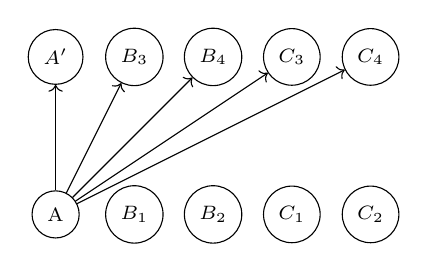
\begin{tikzpicture}[
  scale=1, 
  every node/.style={
    circle, 
    draw=black, 
    fill=white, 
    minimum size=0.4cm, 
    font=\scriptsize
  },
  arrow/.style={->}
]
  \node (A)  at (0,0) {A};
  \node (B1) at (1,0) {$B_{1}$};
  \node (B2) at (2,0) {$B_{2}$};
  \node (C1) at (3,0) {$C_{1}$};
  \node (C2) at (4,0) {$C_{2}$};

  \node (Aprime) at (0,2) {$A'$};
  \node (B3)     at (1,2) {$B_{3}$};
  \node (B4)     at (2,2) {$B_{4}$};
  \node (C3)     at (3,2) {$C_{3}$};
  \node (C4)     at (4,2) {$C_{4}$};

  \draw[arrow] (A) -- (Aprime);
  \draw[arrow] (A) -- (B3);
  \draw[arrow] (A) -- (B4);
  \draw[arrow] (A) -- (C3);
  \draw[arrow] (A) -- (C4);

\end{tikzpicture}
\caption{Dependency graph}
\end{subfigure}
\hfill
\begin{subfigure}[b]{0.7\linewidth}
\centering
\begin{tabular}{|c|c|c|c|c|c|c|c|c|c|c|}
\hline
 & A & A' & $B_{1}$ & $B_{2}$ & $B_{3}$ & $B_{4}$ & $C_{1}$ & $C_{2}$ & $C_{3}$ & $C_{4}$ \\
\hline
\textbf{p} 
  & 21 
  & 21 
  & \multicolumn{4}{c|}{40} 
  & \multicolumn{4}{c|}{18} \\
\textbf{R} 
  & 2   
  & 2.6 
  & \multicolumn{4}{c|}{2} 
  & \multicolumn{4}{c|}{1.5} \\
\hline
\textbf{p'} 
  & 21 
  & \textcolor{red}{18}        
  & \textcolor{red}{22} & \textcolor{red}{22} & \textcolor{red}{18} & \textcolor{red}{18}
  & 18 & 18 & 18 & 18 \\
\textbf{t} 
  & 36 
  & 50 
  & 20 & 20 & 22 & 22 
  & 12 & 12 & 13 & 13 \\
$\boldsymbol{t^{\opt}}$ 
  & 24 
  & 24 
  & 12 & 24 & 12 & 24 
  & 12 & 12 & 12 & 12 \\
$\boldsymbol{p^{\opt}}$ 
  & 45 
  & 45 
  & 40 & 15 & 40 & 15 
  & 20 & 20 & 20 & 20 \\
\hline
\end{tabular}
\caption{Tasks parameters}
\end{subfigure}

\end{subfigure}

\vspace{0.3cm}

\begin{subfigure}[b]{0.95\linewidth}
\centering
%-- Second subfigure: online schedule
\begin{subfigure}[b]{0.63\linewidth}
\centering
\hspace{-2cm}
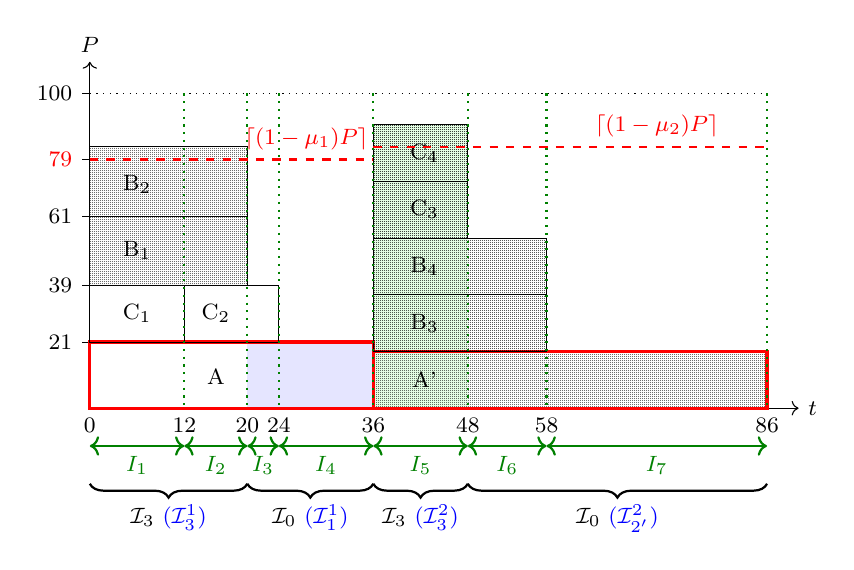
\begin{tikzpicture}[x=0.1cm, y=0.04cm, font=\footnotesize]

  % === Définition d'un motif de hachures légères (pointillées) ===
  \pgfdeclarepatternformonly{lightdots}
    {\pgfpoint{0pt}{0pt}} {\pgfpoint{0.6pt}{0.6pt}} {\pgfpoint{0.6pt}{0.6pt}}{
      \pgfpathcircle{\pgfpoint{0.6pt}{0.6pt}}{0.2pt}
      \pgfusepath{fill}
    }

  % === Zones de fond colorées ===
  \fill[blue!10] (20,0) rectangle +(16,21);

  \fill[green!10] (36,0)  rectangle +(12,18);
  \fill[green!10] (36,18) rectangle +(12,18);
  \fill[green!10] (36,36) rectangle +(12,18);
  \fill[green!10] (36,54) rectangle +(12,18);
  \fill[green!10] (36,72) rectangle +(12,18);

  % === Axes ===
  \draw[->] (0,0) -- (90,0) node[right] {$t$};
  \draw[->] (0,0) -- (0,110) node[above] {$P$};

  % Y-axis ticks updated: 21, 39, 61
  \foreach \y in {21,39,61,100} {
    \draw (0,\y) -- (-1,\y) node[left]{\y};
  }
  \draw (0,79) -- (-1,79) node[left, red]{79};

  % Abscisses
  \foreach \x in {0,12,20,24,36,48,58,86} {
    \draw (\x,0) -- (\x,0) node[below]{\x};
  }

  \draw[dotted] (0,100) -- (86,100);

  % === Tâches ===
  \draw[very thick, draw=red] (0,0) rectangle +(36,21); % A (updated to height=21)

  % Shifted +1 upwards
  \draw (0,21)   rectangle +(12,18); % C1 : p=18
  \draw (12,21)  rectangle +(12,18); % C2

  \draw[pattern=lightdots] (0,39) rectangle +(20,22); % B1 (was 38)
  \draw[pattern=lightdots] (0,61) rectangle +(20,22); % B2 (was 60)

  % A'
  \draw[very thick, draw=red, pattern=lightdots] (36,0) rectangle +(50,18);

  \draw[pattern=lightdots] (36,18) rectangle +(22,18); % B3
  \draw[pattern=lightdots] (36,36) rectangle +(22,18); % B4
  \draw[pattern=lightdots] (36,54) rectangle +(12,18); % C3
  \draw[pattern=lightdots] (36,72) rectangle +(12,18); % C4

  % === Labels ===
  \node at (6,30)  {C\textsubscript{1}};
  \node at (16,30) {C\textsubscript{2}};
  \node at (6,50)  {B\textsubscript{1}};
  \node at (6,71)  {B\textsubscript{2}};
  \node at (42.5,27) {B\textsubscript{3}};
  \node at (42.5,45) {B\textsubscript{4}};
  \node at (42.5,63) {C\textsubscript{3}};
  \node at (42.5,81) {C\textsubscript{4}};
  \node at (16,10)  {A};
  \node at (42.5,9) {A'};

  % === Lignes horizontales de ratio ===
  \draw[red, dashed, thick] (0,79) -- (36,79);
    \node[above, text=red] at (27.5,79) {$\lceil (1-\mu_{1}) P\rceil$};
  \draw[red, dashed, thick] (36,83) -- (86,83);
    \node[above, text=red] at (72,83) {$\lceil (1-\mu_{2}) P\rceil$};

  % === Bornes verticales ===
  \foreach \xx in {12,20,24,36,48,58,86} {
    \draw[green!50!black, dotted, thick] (\xx,100) -- (\xx,0);
  }

  % === Flèches d'intervalles ===
  \draw[<->, thick, color=green!50!black] (0,-12) -- (12,-12)
    node[midway, below, text=green!50!black] {$I_1$};
  \draw[<->, thick, color=green!50!black] (12,-12) -- (20,-12)
    node[midway, below, text=green!50!black] {$I_2$};
  \draw[<->, thick, color=green!50!black] (20,-12) -- (24,-12)
    node[midway, below, text=green!50!black] {$I_3$};
  \draw[<->, thick, color=green!50!black] (24,-12) -- (36,-12)
    node[midway, below, text=green!50!black] {$I_4$};
  \draw[<->, thick, color=green!50!black] (36,-12) -- (48,-12)
    node[midway, below, text=green!50!black] {$I_5$};
  \draw[<->, thick, color=green!50!black] (48,-12) -- (58,-12)
    node[midway, below, text=green!50!black] {$I_6$};
  \draw[<->, thick, color=green!50!black] (58,-12) -- (86,-12)
    node[midway, below, text=green!50!black] {$I_7$};

  % === Intervalles annotés ===
  \draw[decorate, decoration={brace, mirror, amplitude=5pt}, thick] (0,-24) -- (20,-24)
    node[midway, below=4pt, black]
      {$\mathcal{I}_{3}$ \textcolor{blue}{($\mathcal{I}_{3}^{1}$)}};

  \draw[decorate, decoration={brace, mirror, amplitude=5pt}, thick] (20,-24) -- (36,-24)
    node[midway, below=4pt, black]
      {$\mathcal{I}_{0}$ \textcolor{blue}{($\mathcal{I}_{1}^{1}$)}};

  \draw[decorate, decoration={brace, mirror, amplitude=5pt}, thick] (36,-24) -- (48,-24)
    node[midway, below=4pt, black]
      {$\mathcal{I}_{3}$ \textcolor{blue}{($\mathcal{I}_{3}^{2}$)}};

  \draw[decorate, decoration={brace, mirror, amplitude=5pt}, thick] (48,-24) -- (86,-24)
    node[midway, below=4pt, black]
      {$\mathcal{I}_{0}$ \textcolor{blue}{($\mathcal{I}_{2'}^{2}$)}};

\end{tikzpicture}
\caption{\fair schedule}
\end{subfigure}
%-- Third subfigure: optimal schedule
\begin{subfigure}[b]{0.33\linewidth}
\hspace{-2cm}
\centering
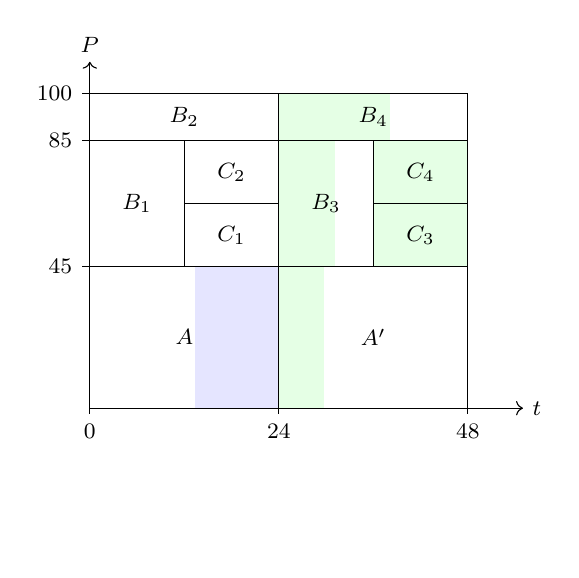
\begin{tikzpicture}[x=0.1cm, y=0.04cm, draw=black, font=\footnotesize]

  \fill[blue!10] (13.33,0) rectangle +(10.67,45);
  \fill[green!10] (24,0) rectangle +(5.76,45);
  \fill[green!10] (24,45) rectangle +(7.08,40);
  \fill[green!10] (24,85) rectangle +(14.16,15);
  \fill[green!10] (36,45) rectangle +(12,20);
  \fill[green!10] (36,65) rectangle +(12,20);

  \draw[->] (0,0) -- (55,0) node[right] {$t$};
  \draw[->] (0,0) -- (0,110) node[above] {$P$};

  \foreach \x in {0,24,48} {
    \draw (\x,0) -- (\x,-2) node[below]{\x};
  }
  \foreach \y in {45,85,100} {
    \draw (0,\y) -- (-1,\y) node[left]{\y};
  }

  \draw (0,0)   rectangle +(24,45) node[midway] {$A$};
  \draw (0,45)  rectangle +(12,40) node[midway] {$B_{1}$};
  \draw (12,45) rectangle +(12,20) node[midway] {$C_{1}$};
  \draw (12,65) rectangle +(12,20) node[midway] {$C_{2}$};
  \draw (0,85)  rectangle +(24,15) node[midway] {$B_{2}$};

  \draw (24,0)  rectangle +(24,45) node[midway] {$A'$};
  \draw (24,45) rectangle +(12,40) node[midway] {$B_{3}$};
  \draw (36,45) rectangle +(12,20) node[midway] {$C_{3}$};
  \draw (36,65) rectangle +(12,20) node[midway] {$C_{4}$};
  \draw (24,85) rectangle +(24,15) node[midway] {$B_{4}$};
  \draw[<->, thick, color=white	] (49,-30) -- (50,-30)
    node[midway, below, text=white] {$\mathcal{I}_{2'}^{2}$};
\end{tikzpicture}

\caption{Optimal schedule}
\end{subfigure}
\end{subfigure}

\caption{Overview of all introduced notations using an example. Top: (a) dependency graph and (b) summary table of execution time and processor allocation. Bottom: (c) \fair schedule and (d) optimal schedule.}
\label{fig:merged_schedule}
\end{figure}

The intuition is as follows.  
The total time spent in $\mathcal{I}_0$ is limited, because there is always at
least one task from a fixed path running during these intervals; hence that
time cannot exceed the processing time of the path itself.
Similarly, the time spent in $\mathcal{I}_3$ is bounded, since the algorithm
processes the graph efficiently in that
high-utilisation regime. By design, \fair balances the allocation such that both execution time and area as are close as possible from the optima, hence these two facts provide the starting point for bounding the overall
makespan.


\paragraph{Example } To illustrate these concepts, we consider the example provided in Figure~\ref{fig:merged_schedule}, which shows in (a) an instance of a task dependency graph. The task graph is composed of ten tasks structured in two layers: the first row contains the independent tasks $A$, $B_1$, $B_2$, $C_1$, and $C_2$, while the second row includes tasks $A'$, $B_3$, $B_4$, $C_3$, and $C_4$, all of which depend on task $A$ as a prerequisite. That is, none of the second-row tasks can be launched before task $A$ has completed. All the $B_i$ (resp. $C_i$) are identical tasks, hence the values (p,R) computed by \textsc{Compute\_Ratio}($j$) are also identical.

The schedule produced by the \textsc{Fair} algorithm for this instance is shown in (c), while an optimal schedule is shown in (d). The platform comprises $P = 100$ processors. According to the summary table in (b), the values of $p_j$ and $\ratio_j$ for each task are determined by the function \textsc{Compute\_Ratio}($j$). At time $t=0$, the available tasks are $A$, $B_1$, $B_2$, $C_1$, and $C_2$, among which the maximum ratio is $\ratio = 2$ (see the second row of the table), resulting in a threshold of $\lceil \mu_1 P \rceil = 22$ : no task can be allocated more than $22$ processors. For this reason, $B_1$ and $B_2$ were \textbf{reduced} to $22$ processors, and $p' \neq p$, which is represented in red in the table and visually indicated in the schedule in (c) by shaded boxes for the affected tasks.

Following the algorithm, tasks $A$, $B_1$, $B_2$, and $C_1$ are launched first. At this point, only 17 processors remain available, which correspond to a high processor allocation (above the red dotted $\lceil (1-\mu_1) P \rceil$ line), hence we are in $\mathcal{I}_0$. The amount of processor available is insufficient to launch $C_2$, which must stay in the queue until more processors are available at $t=12$. From $t=20$ until $A$ completes at $t=20$, the total processor usage falls below $(1-\mu_1) P$, directly implying that no tasks are available, otherwise one would have been launched by $\fair$.

At time $t=36$, task $A$ completes, releasing processors and making its dependent successors $A'$, $B_3$, $B_4$, $C_3$, and $C_4$ available. Among these, the maximum ratio is now $\ratio = 2.6$, as shown in the table, which updates the threshold to $\lceil \mu_2 P \rceil = 18$, so tasks may not be scheduled on more than 18 processors. Many of these tasks had larger original allocations (see row $p$ in the table), and are thus reduced to respect the new threshold $\lceil \mu_2 P \rceil$, resulting in the adjusted allocations $p'_j$ shown in red in the corresponding row.  

Since enough processors are available at $t=36$, all five newly available tasks can be launched simultaneously. Although the queue is empty, the processor usage is above $\lceil (1-\mu_2) P \rceil$. By $t=48$, the processor usage again drops below $\lceil (1-\mu_2) P \rceil$ and the waiting queue is empty. The execution then continues until completion at time $t=86$.

As described earlier, the schedule is partitioned into a sequence of intervals $I_1, I_2, \dots$, each bounded by task start or end events. Within each interval, both the number of processors in use $p(I)$ and the value $\mu_I = \mu(\ratio(I))$ remain constant. Intervals for which $p(I) \geq \lceil (1 - \mu_I) P \rceil$ are classified in $\mathcal{I}_3$, representing high utilization phases, while those with $p(I) < \lceil (1 - \mu_I) P \rceil$ fall into $\mathcal{I}_0$, corresponding to underutilization. As established in Lemma~\ref{lem.I0_path}, during any interval in $\mathcal{I}_0$, the waiting queue is empty and there exists a path in the task graph such that one task from the path is always running. In this example, the path $A \rightarrow A'$ covers the two $\mathcal{I}_0$ intervals in the schedule.



\paragraph{Further Interval Subdivisions }Next, we define a sequence of times \(t_0 = 0 < t_1 < t_2 < \cdots < t_{m-1} < t_m = T\), where each \(t_k\) (for \(k = 1, \dots, m-1\)) marks a task completion at which \(\rratio\) is updated, and \(t_m = T\) is the makespan. Since \(\rratio\) updates occur only upon task completions and there are \(n\) tasks, we have \(m \leq n\), a finite number. We subdivide the set of intervals \(\mathcal{I}\) into \(m\) subsets defined by
\[
\mathcal{I}^k = \{ I \in \mathcal{I} \mid I \subseteq [t_{k-1}, t_k] \}, \quad k = 1, 2, \dots, m,
\]
so that \((\mathcal{I}^k)_{k=1}^m\) forms a partition of \(\mathcal{I}\).

We then define 
\[
\mathcal{I}_3^k = \mathcal{I}_3 \cap \mathcal{I}^k \quad \text{and} \quad \mathcal{I}_0^k = \mathcal{I}_0 \cap \mathcal{I}^k,\quad k = 1,2,\dots,m,
\]
which denote the intervals of \(\mathcal{I}_0\) and \(\mathcal{I}_3\) that lie within the time period \([t_{k-1}, t_k]\), respectively. In each \(\mathcal{I}_0^k\) and \(\mathcal{I}_3^k\), the value \(\rratio(I)\) remains constant (denoted by \(\rratio_k\)) and so does \(\mu(\rratio(I))\) (denoted by \(\mu_k\)). We have $\rratio_1<\rratio_2<\cdots<\rratio_m=\ratio$, since it corresponds to the maximum ratio at the end of the schedule. Note that \(\mathcal{I}_0\) and \(\mathcal{I}_3\) partition \(\mathcal{I}\), while the \((\mathcal{I}_0^k)_{k=1}^m\) and \((\mathcal{I}_3^k)_{k=1}^m\) partition \(\mathcal{I}_0\) and \(\mathcal{I}_3\), respectively.



Using the path $f$ from Lemma~\ref{lem.I0_path}, we further categorize each $\mathcal{I}_0^k$ into two subcategories based on the processor allocation decisions made by \textsc{Fair}:

\begin{itemize}
    \item $\mathcal{I}_1^k$: Intervals in $\mathcal{I}_0^k$ where the task from $f$ running retains its initial processor allocation $p_j$, as computed by \texttt{Compute\_Ratio} (not reduced in line 10 of Algorithm~\ref{alg.online}).
    \item $\mathcal{I}_2^k$: Intervals in $\mathcal{I}_0^k$ where the task from $f$ running has its processor allocation reduced to $\lceil \mu_k P \rceil$ processors (line 10 of Algorithm~\ref{alg.online}).
\end{itemize}


To compare with an optimal offline schedule, we split $\mathcal{I}_2^k$ further:

\begin{itemize}
    \item $\mathcal{I}_{2'}^k$: Intervals in $\mathcal{I}_2^k$ where the task from $f$ running is allocated strictly fewer processors than in the optimal schedule.
    \item $\mathcal{I}_{2''}^k$: Intervals in $\mathcal{I}_2^k$ where the task from $f$ running is allocated at least as many processors as in the optimal schedule.
\end{itemize}
\vspace{0.3cm}

To provide a clearer understanding of the impact of each interval type on the performance of the \textsc{Fair} algorithm, we now give an intuitive explanation of their behavior:

\begin{itemize}
    \item In intervals \( \mathcal{I}_1^k \), the task from path \( f \) is allocated the full processor count \( p_j \) as selected by \texttt{Compute\_Ratio}, without any reduction. By construction, this allocation guarantees that both the execution time and the area are within a factor \( \rratio_k \) of their respective minima. Consequently, the task progresses along path \( f \) at most \( \rratio_k \) times more slowly than in the optimal schedule.
    
    \item In intervals \( \mathcal{I}_{2'}^k \), the task from \( f \) is reduced to \( \lceil \mu_k P \rceil \) processors, which is fewer than its allocation in the optimal schedule. As we assume no superlinear speedup, the execution of the task in f progresses at most \( \mu_k \) times slower than in the optimal (assuming in the worst case scenario that the optimal uses all $P$ processors with perfect speedup). Moreover, the area progresses at most \( \rratio_k / \mu_k \) times more slowly than in the optimal schedule, because the allocation for this task given by \texttt{Compute\_Ratio} remains within a factor \( \rratio_k \) of its minimum area, and the allocation is reduced compared to its original value, which may only decrease the area. Since at least $\mu_k P$ processors are used, no schedule may use more than $\frac{1}{\mu_k}$ times more processors, while being at most $\rratio_k$ times more efficient with the processors.
    
    \item In intervals \( \mathcal{I}_{2''}^k \), the task from \( f \) is again reduced to \( \lceil \mu_k P \rceil \) processors, but this time receives at least as many processors as in the optimal schedule. Thus, progress along the path is guaranteed to be no worse than that in the optimal using the monotonicity assumption, and the efficiency for the area is again no worse than a factor \( \rratio_k / \mu_k \) from the optimal.
    
    \item Finally, in intervals \( \mathcal{I}_3^k \), at least \( (1 - \mu_k)P \) processors are active. Since all running tasks have been allocated in a way that ensures an area within a factor \( \rratio_k \) of the minimum, the aggregate area consumption is at most \( \rratio_k / (1 - \mu_k) \) times slower than the corresponding area in the optimal schedule.
    
\end{itemize}

This refined classification will allow the derivation of bounds involving $\frac{A^{\opt}}{P}$ and $C^{\opt}$ , while accounting for the varying values of \( \rratio_k \) that arise dynamically in the execution of \textsc{Fair}. This analysis builds upon the methodology introduced in~\cite{TOPC24}, but extends it to accommodate the variation of the reduction step in Line 10 of Algorithm~\ref{alg.online}, which was not addressed in earlier work.

\vspace{0.3cm}

For each interval $I$, let $|I|$ denote its duration. We define the total durations of each category within period $k$:
\[
T_1^k = \sum_{I \in \mathcal{I}_1^k} |I|, \quad T_2^k = \sum_{I \in \mathcal{I}_2^k} |I|, \quad T_{2'}^k = \sum_{I \in \mathcal{I}_{2'}^k} |I|, \quad T_{2''}^k = \sum_{I \in \mathcal{I}_{2''}^k} |I|, \quad T_3^k = \sum_{I \in \mathcal{I}_3^k} |I|.
\]
Given the partitioning properties—$\mathcal{I}_0$ and $\mathcal{I}_3$ partition $\mathcal{I}$, $(\mathcal{I}_0^k)_{k=1}^m$ partition $\mathcal{I}_0$, $(\mathcal{I}_3^k)_{k=1}^m$ partition $\mathcal{I}_3$, $\mathcal{I}_1^k$ and $\mathcal{I}_2^k$ partition $\mathcal{I}_0^k$, and $\mathcal{I}_{2'}^k$ and $\mathcal{I}_{2''}^k$ partition $\mathcal{I}_2^k$—the makespan is:
\[
T = \sum_{k=1}^m (T_1^k + T_2^k + T_3^k).
\]

This structured decomposition enables a detailed worst-case performance analysis of \textsc{Fair} by examining the contributions of each interval category to the makespan $T$.

In the rest of the analysis, we will build upper bounds that will be used to replace the $T_1^k$, $T_2^k$ and $T_3^k$ to eventually show that $T \leq \frac{T_{opt}}{\mu(\ratio)}$, where $\ratio$ corresponds to the largest ratio among all tasks.

Additionally, for each $k$, since $T_2^k = T_{2'}^k + T_{2''}^k$, we introduce $z_k \in [0,1]$ such that:
\begin{equation}
\label{eq.zk}
T_{2'}^k = z_k T_2^k, \quad T_{2''}^k = (1 - z_k) T_2^k
\end{equation}
quantifying the proportion of $\mathcal{I}_2^k$ where the algorithm under-allocates processors for tasks in the path $f$ compared to the optimal and vice versa.

Finally, for each period \( k \), we define the total time task \( j \) runs within \( \mathcal{I}^{k} \) in the \textsc{Fair} schedule: \[ T_{j}^{k} = \sum_{I \in \mathcal{I}^{k}} |I \cap [s_j, e_j]| \]. Similarly, we can subdivide this length based on the partition of $\mathcal{I}^{k}$:
\[
T_{j,1}^{k} = \sum_{I \in \mathcal{I}_{1}^{k}} |I \cap [s_j, e_j]|
\quad T_{j,2'}^{k} = \sum_{I \in \mathcal{I}_{2'}^{k}} |I \cap [s_j, e_j]|,\quad
T_{j,2''}^{k} = \sum_{I \in \mathcal{I}_{2''}^{k}} |I \cap [s_j, e_j]|,\quad
T_{j,3}^{k} = \sum_{I \in \mathcal{I}_{3}^{k}} |I \cap [s_j, e_j]|.
\]
For example, \(T_{j,2'}^{k}\) corresponds to the total amount of time where task \(j\) runs within the intervals in \(\mathcal{I}_{2'}^{k}\).
\medskip



\paragraph{Example} In the example of Figure~\ref{fig:merged_schedule}, there is a single update to the value of $\rratio$ during the schedule: it increases from $\rratio_1 = 2$ to $\rratio_2 = 2.6$ when task $A'$ becomes available at time $t=36$. This creates a subdivision of the time axis into two intervals: $[0,36]$ and $[36,86]$, corresponding to $k = 1$ and $k = 2$, respectively, so $m=2$.

The first high-utilization phase, $I_3$ from $[0,20]$ (highlighted in blue in the figure), belongs to $\mathcal{I}_3^1$. The following interval $[20,36]$ falls into $\mathcal{I}_1^1$, and since task $A$—the task from path $f = A \rightarrow A'$ running during this interval—retains its original allocation (i.e., it is not reduced), this interval belongs to $\mathcal{I}_1^1$.

The second high-utilization phase, from $[36,48]$, is part of $\mathcal{I}_3^2$. Finally, the last phase from $[48,86]$ belongs to $\mathcal{I}_0^2$. During this period, task $A'$ from path $f$ is running with a reduced processor allocation $p' = 18$, which is strictly less than the $p^{\opt} = 45$ processors used in the optimal schedule (see table (b) and schedule (d)). Therefore, this interval belongs to $\mathcal{I}_{2'}^2$.

In this simple example, each category contains only a single interval, so the corresponding durations $T_3^1$, $T_{1}^1$,  $T_3^2$ and $T_{2'}^2$, can be directly read as the lengths of those intervals: $20, 16, 12$ and $38$, respectively. In general, these totals are obtained by summing the lengths of all intervals in each category, even when they are non-contiguous. Any other interval type, such as $I_{2'}^1$ is not represented in this example and $T_{2'}^1=0$.

Let us now consider the execution time of task $A$ within these subdivisions. Task $A$ starts at $t=0$ and completes at $t=36$, intersecting both the interval in $\mathcal{I}_3^1$ and the one in $\mathcal{I}_1^1$. The duration of $A$ overlapping with the first high-utilization interval ($I_3^1$) is $|[0,20]| = 20$, which gives $T_{A,3}^1 = 20$. Similarly, the duration overlapping with the underutilized interval ($\mathcal{I}_1^1$) is $|[20,36]| = 16$, giving $T_{A,1}^1 = 16$. For other interval categories, either the one that appears in the schedule where $A$ doesn't intersect, such as $\mathcal{I}_3^2$; or the ones that don't appear, the corresponding time is $0$. For instance, $T_{A,2''}^1 = T_{A,3}^2 = 0$.

This breakdown highlights how each interval contributes to the makespan and to the execution timeline of individual tasks in the path $f$. Such fine-grained decomposition is essential to derive performance bounds for the \textsc{Fair} algorithm.



\subsubsection{Areas}
To analyze the worst-case performance of the \textsc{Fair} algorithm, we introduce area-based metrics that quantify the resource utilization of tasks during specific intervals within each period \( k \). These metrics enable a comparison between the \textsc{Fair} schedule and an optimal schedule, supporting the derivation of upper bounds on the makespan \( T \).

\paragraph{Areas in the \textsc{Fair} Schedule}


The areas associated with tasks in the path \( f \) in the \textsc{Fair} schedule are defined as
\[
A_{2'|f}^{k} = \sum_{j \in f} p'_j\, T_{j,2'}^{k},\quad
A_{2''|f}^{k} = \sum_{j \in f} p'_j\, T_{j,2''}^{k},\quad
A_{3}^{k} = \sum_{j=1}^{n} p'_j\, T_{j,3}^{k},
\]
where \(p'_j\) denotes the number of processors allocated to task \(j\) in the \textsc{Fair} schedule. Note that we only include tasks in the path $f$ for $A_{2'|f}^{k}$ and $A_{2''|f}^{k}$. The reason is that, in the worst case, no other task may be running during
intervals of type \(\mathcal{I}_{2'}^{k}\) or \(\mathcal{I}_{2''}^{k}\); hence
including additional tasks would not tighten the competitive‐ratio bound.
Conversely, all tasks are taken into account in \(A_{3}^{k}\).
These definitions capture the resource utilization of tasks during the subintervals of period \( k \) in the \textsc{Fair} schedule.


\paragraph{Areas in the Optimal Schedule}
To facilitate comparison, we define corresponding areas in the optimal schedule based on the proportional execution times of tasks in the \textsc{Fair} schedule. In particular, we define
\[
A^{k,\opt}_{2'|f} = \sum_{j \in f} \frac{T_{j,2'}^{k}}{t_j(p'_j)} a_j^{\opt},\quad
A^{k,\opt}_{2''|f} = \sum_{j \in f} \frac{T_{j,2''}^{k}}{t_j(p'_j)} a_j^{\opt},\quad
A^{k,\opt}_{3} = \sum_{j=1}^{n} \frac{T_{j,3}^{k}}{t_j(p'_j)} a_j^{\opt},\quad 
A^{k,\opt} = \sum_{j=1}^{n} \frac{T_{j}^{k}}{t_j(p'_j)} a_j^{\opt}
\]
where \(a_j^{\opt} = p_j^{\opt} t_j(p_j^{\opt})\) is the area of task \(j\) in the optimal schedule, \(p_j^{\opt}\) denotes the optimal processor allocation, and \(t_j(p'_j)\) is the execution time of task \(j\) with \(p'_j\) processors in the \textsc{Fair} schedule. These definitions capture the proportional areas in the optimal schedule corresponding to the time spent in the intervals \(\mathcal{I}_{2'}^{k}\), \(\mathcal{I}_{2''}^{k}\), \(\mathcal{I}_{3}^{k}\), and \(\mathcal{I}^{k}\) respectively, in the \fair schedule.



\paragraph{Example}

In the example of Figure~\ref{fig:merged_schedule}, (c) and (d), we illustrate in green the area calculations for $A_3^2$ in the \textsc{Fair} schedule (left), and $A_3^{2,\opt}$ in the optimal schedule (right). These quantities correspond to the total processor-time product (i.e., area) used by all tasks during the high-utilization interval $I_3^2 = [36,48]$.

To compute $A_3^2$, we consider all tasks that are running during $I_3^2$ in the \textsc{Fair} schedule. This includes tasks $C_3$ and $C_4$, which are fully contained in this interval and use 18 processors each. In addition, tasks $B_3$ and $B_4$ overlap partially with $I_3^2$: they run for 22 time units total, and only the first 12 time units lie within $I_3^2$. Therefore, each of them contributes $\frac{12}{22}$ of its area. Finally, task $A'$ overlaps $I_3^2$ for its first 12 units of execution out of 50 total, contributing $\frac{12}{50}$ of its area. The total area in \textsc{Fair} is thus:
\[
A_3^2 = a_{C_3} + a_{C_4} + \frac{12}{22}(a_{B_3} + a_{B_4}) + \frac{12}{50} a_{A'},
\]
where $a_j = p'_j \cdot t_j(p'_j)$ denotes the area of task $j$ in the \textsc{Fair} schedule.

To compute the corresponding area in the optimal schedule, we use the same fractions of execution but apply them to the optimal areas. These tasks are highlighted in green in the optimal schedule (d). The total area is given by:
\[
A_3^{2,\opt} = a_{C_3}^{\opt} + a_{C_4}^{\opt} + \frac{12}{22}(a_{B_3}^{\opt} + a_{B_4}^{\opt}) + \frac{12}{50} a_{A'}^{\opt},
\]
where $a_j^{\opt} = p_j^{\opt} \cdot t_j(p_j^{\opt})$ is the optimal area of task $j$. This definition reflects the idea that the area in the optimal schedule is reconstructed by proportionally allocating task areas according to the fraction of time those tasks run in the \textsc{Fair} schedule during $I_3^2$.

This proportional view enables us to compare processor usage efficiency between \textsc{Fair} and an optimal schedule, interval by interval, and ultimately derive bounds on the total makespan.


\subsubsection{Paths}
Recall that \(T_{j,1}^{k}\) corresponds to the total length of time that task \( j \) runs within the intervals \(\mathcal{I}_{1}^{k}\) in the \textsc{Fair} schedule (resp. \(T_{j,2'}^{k}\), \(T_{j,2''}^{k}\)).
We define the corresponding lengths in the optimal schedule by scaling these durations according to the fraction of task \( j \) executed in the \textsc{Fair} schedule, multiplied by the optimal execution time \( t_j^{\opt} \) for task \( j \):
\[
L^{k,\opt}_{1|f} = \sum_{j \in f} \frac{T_{j,1}^{k}}{t_j(p'_j)} t_j^{\opt},\quad
L^{k,\opt}_{2'|f} = \sum_{j \in f} \frac{T_{j,2'}^{k}}{t_j(p'_j)} t_j^{\opt},\quad
L^{k,\opt}_{2''|f} = \sum_{j \in f} \frac{T_{j,2''}^{k}}{t_j(p'_j)}  t_j^{\opt},\quad
L^{k,\opt}_{f} = \sum_{j \in f} \frac{T_{j}^{k}}{t_j(p'_j)}  t_j^{\opt},
\]
where \( t_j(p'_j) \) denotes the execution time of task \( j \) in the \textsc{Fair} schedule and \( t_j^{\opt} \) its execution time under an optimal schedule. These definition follows exactly the same idea as the area definitions.


\paragraph{Example}

In the example of Figure~\ref{fig:merged_schedule}, (c) and (d), we highlight in blue on the left the portion of the path \( f = A \rightarrow A' \) that overlaps the interval \( I_1^1 = [20,36] \), which is part of \(\mathcal{I}_1^1\). During this interval, only task \( A \) is running on the path \( f \), and it overlaps with the full 16 units of this interval out of its total execution time of 36 in the \textsc{Fair} schedule. Therefore, the proportion of task \( A \) that intersects \(\mathcal{I}_1^1\) is \(\frac{16}{36}\).

To compute the corresponding optimal length, we use this fraction scaled by the optimal execution time of \( A \), yielding:
\[
L_{1|f}^{1,\opt} = \frac{16}{36} \cdot t_A^{\opt}.
\]
From the task table (b), we know that \( t_A^{\opt} = 24 \), so this gives \( L_{1|f}^{1,\opt} = \frac{16}{36} \cdot 24 \). In this example, \( A \) is the only task in \( f \) that overlaps \(\mathcal{I}_1^1\), but in general, several tasks along the path may contribute to the sum.\\


This concludes our concrete example-based illustration of the area and path metrics. All the ingredients are now in place to derive the approximation ratio of the \textsc{Fair} algorithm by bounding the total makespan \( T \) in terms of the optimal makespan \( T^{\opt} \). But first, we will list and prove different properties that link the attributes introduced here.




\subsection{Structural Properties of the Schedule}
\begin{table}[h]
\centering
\caption{Crucial properties}
\label{tab.prop}
\renewcommand{\arraystretch}{2}
\begin{tabular}{|c|c|c|}
\hline
\textbf{Global} & \textbf{Area} & \textbf{Path} \\
\hline
\(\frac{x}{1-\mu(x)} = \frac{1}{\mu(x)} - x\) \hfill (G1) & \(\mu_k T_{2'}^k \leq \frac{A_{2'|f}^{k,\opt}}{P}\) \hfill (A1) & \(T_1^k \leq R_k L_{1|f}^{k,\opt}\) \hfill (P1) \\
\hline
\(\frac{x}{1-\mu(x)}\) increases with \(x\) \hfill  (G2) & \(\frac{\mu_k T_{2''}^k}{R_k} \leq \frac{A_{2''|f}^{k,\opt}}{P}\) \hfill (A2) & \(T_{2'}^k \leq \frac{L_{2'|f}^{k,\opt}}{\mu_k}\) \hfill (P2) \\
\hline
\(\mu(x)\) decreases with \(x\) \hfill(G3) & \(\frac{(1 - \mu_k) T_3^k}{R_k} \leq \frac{A_3^{k,\opt}}{P}\) \hfill (A3) & \(T_{2''}^k \leq L_{2''|f}^{k,\opt}\) \hfill (P3) \\
\hline
\(\mu_k \leq \frac{3 - \sqrt{5}}{2}\)
 \hfill (G4) & \(A_{2'|f}^{k,\opt} + A_{2''|f}^{k,\opt} + A_3^{k,\opt} \leq A^{k,\opt}\) \hfill (A4) & \(L_{1|f}^{k,\opt} + L_{2'}^{k,\opt} + L_{2''}^{k,\opt} \leq L_f^{k,\opt}\) \hfill (P4) \\
\hline
\(T_2^k = \frac{T_{2'}^k}{z_k} = \frac{T_{2''}^k}{1 - z_k}\) \hfill (G5) & \(\sum_{k=1}^m A^{k,\opt} \leq T^{\opt}\) \hfill (A5) & \(\sum_{k=1}^m L_f^{k,\opt} \leq T^{\opt}\) \hfill (P5) \\
\hline
\end{tabular}
\end{table}

Table~\ref{tab.prop} collects several useful properties that are repeatedly used throughout the analysis. By grouping them in one place, we streamline the presentation of more involved derivations and avoid interrupting the main proofs with technical but straightforward steps. All properties listed in the table will be formally proved in this section.

\paragraph{Global} 

Recall that the function $\mu$ is defined for $x \geq 1$ as $\mu(x)=\frac{2x+1-\sqrt{4x^2+1}}{2x}$. Hence, $\mu(x)$ has the same sign as $2x+1-\sqrt{4x^2+1} > 2x+1-\sqrt{4x^2+4x+1}=0$, hence it is well defined and positive. To show the Global results, we first define $v(x)=\frac{x}{1-\mu(x)}$
\begin{align*}
v(x)&=\frac{x}{1-\mu(x)}=\frac{x}{\frac{\sqrt{4x^2+1}-1}{2x}}= \frac{2x^2}{\sqrt{4x^2+1}-1}=\frac{2x^2(\sqrt{4x^2+1}+1)}{4x^2+1-1}=\frac{\sqrt{4x^2+1}+1}{2}\\
&= \frac{2x+1+\sqrt{4x^2+1}}{2}-x=\frac{(2x+1+\sqrt{4x^2+1})(2x+1+\sqrt{4x^2+1})}{2(2x+1-\sqrt{4x^2+1})}-x \\
&= \frac{(2x+1)^2-(4x^2+1)}{2(2x+1-\sqrt{4x^2+1})}-x = \frac{2x}{2x+1-\sqrt{4x^2+1}}-x = \frac{1}{\mu(x)}-x.\quad \text{(G1 \checkmark)}
\end{align*}

Since $v(x)= \frac{\sqrt{4x^2+1}+1}{2}$ (first line, last equality), we see that $v(x)$ is increasing (G2 \checkmark), and with $v(x)=\frac{1}{\mu(x)}-x$, we have shown $\frac{1}{\mu(x)}$ must increase since $v(x)$ increases and $-x$ decreases with $x$. Thus $\mu(x)$ decreases with $x$ (G3 \checkmark). Finally since the ratio is always larger than $1$, $\mu(x) \leq \mu(1) = \frac{3-\sqrt{5}}{2}$ (G4 \checkmark). Using Equation~\ref{eq.zk}, we directly have G5 \checkmark: it is simply the definition of $z_k$ restated here for convenience.

\paragraph{Area} For convenience we reproduce the area definitions: \(
A_{2'|f}^{k} = \sum_{j \in f} p'_j\, T_{j,2'}^{k},
A_{2''|f}^{k} = \sum_{j \in f} p'_j\, T_{j,2''}^{k},
A_{3}^{k} = \sum_{j=1}^{n} p'_j\, T_{j,3}^{k},
\) and \(
A^{k,\opt}_{2'|f} = \sum_{j \in f} \frac{T_{j,2'}^{k}}{t_j(p'_j)} a_j^{\opt},
A^{k,\opt}_{2''|f} = \sum_{j \in f} \frac{T_{j,2''}^{k}}{t_j(p'_j)} a_j^{\opt},
A^{k,\opt}_{3} = \sum_{j=1}^{n} \frac{T_{j,3}^{k}}{t_j(p'_j)} a_j^{\opt}, 
A^{k,\opt} = \sum_{j=1}^{n} \frac{T_{j}^{k}}{t_j(p'_j)} a_j^{\opt}
\).

\paragraph{(A1)} In subintervals of $\mathcal{I}_{2'}^k$, tasks from path $f$ utilize at least $\mu_k P$ processors (by definition). Thus, we have:
\[
\mu_k P\, T_{2'}^k \;\le\; A_{2'|f}^{k} = \sum_{j \in f} p'_j T_{j,2'}^k = \sum_{j \in f} \frac{a_j(p'_j)}{t_j(p'_j)}T_{j,2'}^k \le \sum_{j \in f}\frac{a_j(p_j^{\opt})}{t_j(p'_j)}T_{j,2'}^k = A_{2'|f}^{k,\opt},
\]
where the inequality follows from the fact that area is non-decreasing with processor allocation: by definition, in $\mathcal{I}_{2'}^k$, all tasks $j$ from path $f$ are allocated fewer processors than in the optimal, hence \(a_j(p'_j) \le a_j(p_j^{\opt})\). Dividing by \(P\), we obtain:
\[
\mu_k T_{2'}^k \;\le\; \frac{A_{2'|f}^{k,\opt}}{P} \quad \text{(A1 \checkmark)}.
\]

\paragraph{(A2)} Again, in subintervals of $\mathcal{I}_{2''}^k$, tasks from $f$ occupy at least $\mu_k P$ processors. Then:
\[
\mu_k P\, T_{2''}^k \le A_{2''|f}^{k} = \sum_{j \in f} p'_j T_{j,2''}^k = \sum_{j \in f} \frac{a_j(p'_j)}{t_j(p'_j)}T_{j,2''}^k \le \sum_{j \in f} \frac{\rratio_k  a_j^{\opt}}{t_j(p'_j)} T_{j,2''}^k = \rratio_k A_{2''|f}^{k,\opt},
\]
This time, using the bound \(a_j(p'_j) \le a_j(p_j) \le \rratio_k a_j^{\min} \le \rratio_k a_j^{\opt}\). All tasks in $f$ processed in $\mathcal{I}_{2''}^k$ are a factor $\rratio_k$ away from the minimal area before reduction, hence it is still the case after reduction. Dividing by \(\rratio_k P\) yields:
\[
\frac{\mu_k T_{2''}^k}{\rratio_k} \le \frac{A_{2''|f}^{k,\opt}}{P} \quad \text{(A2 \checkmark)}.
\]

\paragraph{(A3)} In subintervals $\mathcal{I}_{3}^k$, at least $(1 - \mu_k)P$ processors are used. We obtain:
\[
(1-\mu_k)P T_3^k \le A_3^k = \sum_{j=1}^{n} p'_j T_{j,3}^k = \sum_{j=1}^{n} \frac{a_j(p'_j)}{t_j(p'_j)}T_{j,3}^k \le  \sum_{j=1}^{n} \frac{\rratio_k a_j^{\opt}}{t_j(p'_j)} T_{j,3}^k = \rratio_k A_3^{k,\opt}.
\]
For the same reason as in (A2), the bound \(a_j(p'_j) \le \rratio_k a_j^{\opt}\) holds. Dividing by $\rratio_k P$ gives:
\[
\frac{(1 - \mu_k) T_3^k}{\rratio_k} \le \frac{A_3^{k,\opt}}{P} \quad \text{(A3 \checkmark)}.
\]

\paragraph{(A4)} The terms \(A_{2'|f}^{k,\opt}\), \(A_{2''|f}^{k,\opt}\), and \(A_3^{k,\opt}\) correspond to the proportional areas in the optimal schedule corresponding to the time spent in the intervals \(\mathcal{I}_{2'}^{k}\), \(\mathcal{I}_{2''}^{k}\), \(\mathcal{I}_{3}^{k}\), and \(\mathcal{I}^{k}\) respectively, in the \fair schedule. Since \(\mathcal{I}_{2'}^{k}\), \(\mathcal{I}_{2''}^{k}\), \(\mathcal{I}_{3}^{k}\) are disjoint subsets of \(\mathcal{I}^{k}\), all corresponding areas in the optimal schedule also correspond to disjoint fractions of the tasks (see the example in Figure~\ref{fig:merged_schedule}, (c) and (d)). More precisely, $T_{j,2'}^k+T_{j,2''}^{k}+T_{j,3}^{k} \leq T_{j}^{k}$. Hence,
\begin{equation}
 A^{k,\opt}_{2'|f} + A^{k,\opt}_{2''|f} + A^{k,\opt}_{3} \leq \sum_{j \in f} \frac{T_{j,2'}^{k}}{t_j(p'_j)} a_j^{\opt} 
+ \sum_{j \in f} \frac{T_{j,2''}^{k}}{t_j(p'_j)} a_j^{\opt} 
+ \sum_{j=1}^{n} \frac{T_{j,3}^{k}}{t_j(p'_j)} a_j^{\opt}
\;\le\;
\sum_{j=1}^{n} \frac{T_{j}^{k}}{t_j(p'_j)} a_j^{\opt} \leq A^{k,\opt} 
\tag{A4 \checkmark}
\end{equation}


\paragraph{(A5)} Finally, summing over all periods, we have:
\[
 \sum_{k=1}^m A^{k,\opt} = \sum_{k=1}^m \sum_{j=1}^{n} \frac{T_j^k}{t_j(p'_j)} a_j^{\opt}.
\]
Now, for each task \(j\), the total time it is executed over all intervals satisfies \(\sum_{k=1}^m T_j^k = t_j(p'_j)\). Hence:
\[
\sum_{k=1}^m A^{k,\opt} = \sum_{j=1}^n \frac{a_j^{\opt}}{t_j(p'_j)} \sum_{k=1}^m T_j^k = \sum_{j=1}^n a_j^{\opt} = A^{\opt} \quad \text{(A5 \checkmark)}.
\]

\paragraph{Paths} For convenience we reproduce the path definitions: \(
L^{k,\opt}_{1|f} = \sum_{j \in f} \frac{T_{j,1}^{k}}{t_j(p'_j)} t_j^{\opt},\quad
L^{k,\opt}_{2'|f} = \sum_{j \in f} \frac{T_{j,2'}^{k}}{t_j(p'_j)} t_j^{\opt},\quad
L^{k,\opt}_{2''|f} = \sum_{j \in f} \frac{T_{j,2''}^{k}}{t_j(p'_j)}  t_j^{\opt},\quad
L^{k,\opt}_{f} = \sum_{j \in f} \frac{T_{j}^{k}}{t_j(p'_j)}  t_j^{\opt},
\)

\paragraph{(P1)} In subintervals in $\mathcal{I}_1^k$, the schedule executes exactly one task from the path $f$ at all times (by Lemma~\ref{lem.I0_path}, because $\mathcal{I}_1^k \subset \mathcal{I}_0$). Therefore, the total time spent in $\mathcal{I}_1^k$ satisfies:
\[
T_1^k = \sum_{j \in f} T_{j,1}^k,
\]
Again, this is because $T_{j,1}^k$ represents the amount of time spent in $\mathcal{I}_1^k$ by task $j$. No reduction is applied to tasks from $f$ in $\mathcal{I}_1^k$, so by the definition of $\rratio_k$, we have:
\[
t_j(p'_j) \le \rratio_k\, t_j^{\opt},
\]
and hence:
\[
T_1^k = \sum_{j \in f} \frac{T_{j,1}^k}{t_j(p'_j)} t_j(p'_j) \le \rratio_k \sum_{j \in f} \frac{T_{j,1}^k}{t_j(p'_j)} t_j^{\opt} = \rratio_k L_{1|f}^{k,\opt} \quad \text{(P1 \checkmark)}.
\]

\paragraph{(P2)} In subintervals in $\mathcal{I}_{2'}^k$, exactly one task from $f$ is executed at all times. This task is reduced and uses $\lceil \mu_k P\rceil$ processors. Since we assume there is no superlinear speedup, and at most $P$ processors are available, for all task $j$ running in $\mathcal{I}_{2'}^k$, 
\[
t_j(p'_j) \le \frac{t_j^{\opt}}{\mu_k},
\]
Therefore:
\[
T_{2'}^k = \sum_{j \in f} T_{j,2'}^k = \sum_{j \in f} \frac{T_{j,2'}^k}{t_j(p'_j)} t_j(p'_j) \le \sum_{j \in f} \frac{T_{j,2'}^k}{t_j(p'_j)} \cdot \frac{t_j^{\opt}}{\mu_k} = \frac{1}{\mu_k} \sum_{j \in f} \frac{T_{j,2'}^k}{t_j(p'_j)} t_j^{\opt} = \frac{1}{\mu_k} L_{2'|f}^{k,\opt} \quad \text{(P2 \checkmark)}.
\]

\paragraph{(P3)} In subintervals in $\mathcal{I}_{2''}^k$, again one task from $f$ runs at all times, but this time with at least as many processors as in the optimal schedule. Since using more processors can only reduce execution time due to the non-increasing nature of $t_j(p)$ on $[1,p^{\max}_j]$, we have:
\[
t_j(p'_j) \le t_j^{\opt} \Rightarrow T_{2''}^k = \sum_{j \in f} T_{j,2''}^k \le \sum_{j \in f} \frac{T_{j,2''}^k}{t_j(p'_j)} t_j^{\opt} = L_{2''|f}^{k,\opt} \quad \text{(P3 \checkmark)}.
\]

\paragraph{(P4)} Since the intervals in $\mathcal{I}_{1}^k$, $\mathcal{I}_{2'}^k$, and $\mathcal{I}_{2''}^k$ are disjoint, and exactly one task from path $f$ is always running in these intervals. The corresponding optimal lengths can therefore be added:
\[
L_{1|f}^{k,\opt} + L_{2'|f}^{k,\opt} + L_{2''|f}^{k,\opt} \le L_f^{k,\opt} \quad \text{(P4 \checkmark)}.
\]

\paragraph{(P5)} Finally, summing over all $k$:
\[
\sum_{k=1}^m L_f^{k,\opt} = \sum_{k=1}^m \sum_{j \in f} \frac{T_j^k}{t_j(p'_j)} t_j^{\opt}.
\]
For each task $j \in f$, the total time executed over all intervals satisfies $\sum_{k=1}^m T_j^k = t_j(p'_j)$, hence:
\[
\sum_{k=1}^m L_f^{k,\opt} = \sum_{j \in f} \frac{t_j^{\opt}}{t_j(p'_j)} \sum_{k=1}^m T_j^k = \sum_{j \in f} t_j^{\opt} = L_f^{\opt}.
\]
Since the critical path $f$ is a subset of all tasks and the optimal makespan must be at least the length of any path:
\[
\sum_{k=1}^m L_f^{k,\opt} \le T^{\opt} \quad \text{(P5 \checkmark)}.
\]


In the next section, we combine all the results from Table~\ref{tab.prop} with the identity \( T = \sum_{k=1}^m (T_1^k + T_2^k + T_3^k) \) to derive an upper bound on \( T \) in terms of \( T^{\opt} \).

\subsection{Final Ratio Bound}
Before stating the two key lemmas, we pause for a brief recap: many symbols
have been introduced, and it is useful to gather their meaning in one place.

\medskip\noindent
\textbf{Time-partition}  
During each window $[t_{k-1},t_k]$ of the schedule produced by \fair, the
intervals are split into disjoint sets:
$\mathcal{I}_1^k$ (under-utilised, \emph{unreduced} allocations on the path
$f$), $\mathcal{I}_2^k$ (under-utilised, \emph{reduced} allocations, meaning that at least $\lceil \mu_k P \rceil$ processors are used), and
$\mathcal{I}_3^k$ (high utilisation).  
Their total lengths are $T_1^k$, $T_2^k$, and $T_3^k$, respectively.
Inside $\mathcal{I}_2^k$ we further isolate a fraction
$z_k$ where the path task receives fewer processors than in the optimum
($\mathcal{I}_{2'}^k$) and a fraction $1-z_k$ where it receives at least as
many ($\mathcal{I}_{2''}^k$).

\smallskip\noindent
\textbf{Efficiency parameters.}  
$\mu_k=\mu(\rratio_k)$ is the capping ratio that limits any processor
allocation to $\mu_kP$ during period~$k$, while
$\rratio_k\!\ (\ge1)$ is the largest per-task slowdown encountered so
far, both for time and area.  These two quantities measure how far \fair can deviate from an optimal
allocation for these metrics.

\smallskip\noindent
\textbf{Optimal benchmarks.}  
$A^{k,\opt}$ is the amount of area in the optimal
offline schedule that corresponds to the fraction of tasks that \fair executes
inside $[t_{k-1},t_k]$.  Likewise, $L_f^{k,\opt}$ is the time the optimal schedule
spends on the portion of the critical path $f$ corresponding to the work done
by \fair in that window. Together, they allow building bounds with the optimal time of the schedule.

\medskip
Splitting time into $\mathcal{I}_1^k$, $\mathcal{I}_2^k$, and
$\mathcal{I}_3^k$ provides detailed information about \fair{}’s efficiency:
\(\mathcal{I}_1^k\) and \(\mathcal{I}_2^k\) control how fast progress is made
along the critical path, while $\mathcal{I}_2^k$ and \(\mathcal{I}_3^k\) capture how quickly area is
consumed when the platform is highly loaded.  The following two lemmas convert
those local observations into global bounds by relating
$(T_1^k,T_2^k,T_3^k)$ to the optimal references $(A^{k,\opt},L_f^{k,\opt})\), each lemma correspond to one of the bounds.



\begin{lemma}\label{lem.area}
For any $k \in [1,m]$, we have:
\begin{equation}\label{Area}
\mu_k\left( z_k + \frac{1 - z_k}{\rratio_k} \right) T_2^k + \frac{1 - \mu_k}{\rratio_k} T_3^k \le \frac{A^{k,\opt}}{P} \ .
\end{equation}
\end{lemma}

\begin{proof}
From property (G5) in Table~\ref{tab.prop}, we have:
\[
T_2^k = \frac{T_{2'}^k}{z_k} = \frac{T_{2''}^k}{1 - z_k} \quad \Rightarrow \quad T_{2'}^k = z_k T_2^k, \quad T_{2''}^k = (1 - z_k) T_2^k.
\]
Using properties (A1), (A2), and (A3), we obtain:
\[
\mu_k T_{2'}^k \le \frac{A_{2'|f}^{k,\opt}}{P}, \qquad
\frac{\mu_k T_{2''}^k}{\rratio_k} \le \frac{A_{2''|f}^{k,\opt}}{P}, \qquad
\frac{(1 - \mu_k) T_3^k}{\rratio_k} \le \frac{A_3^{k,\opt}}{P}.
\]
Adding these inequalities:
\[
\mu_k T_{2'}^k + \frac{\mu_k T_{2''}^k}{\rratio_k} + \frac{(1 - \mu_k) T_3^k}{\rratio_k}
\le \frac{A_{2'|f}^{k,\opt} + A_{2''|f}^{k,\opt} + A_3^{k,\opt}}{P}.
\]
Then, applying property (A4):
\[
A_{2'|f}^{k,\opt} + A_{2''|f}^{k,\opt} + A_3^{k,\opt} \le A^{k,\opt},
\]
we get:
\[
\mu_k T_{2'}^k + \frac{\mu_k T_{2''}^k}{\rratio_k} + \frac{(1 - \mu_k) T_3^k}{\rratio_k}
\le \frac{A^{k,\opt}}{P}.
\]
Finally, substituting \(T_{2'}^k = z_k T_2^k\) and \(T_{2''}^k = (1 - z_k) T_2^k\) into the left-hand side:
\[
\mu_k \left( z_k + \frac{1 - z_k}{\rratio_k} \right) T_2^k + \frac{1 - \mu_k}{\rratio_k} T_3^k \le \frac{A^{k,\opt}}{P},
\]
which concludes the proof.
\end{proof}

\begin{lemma}\label{lem.path}
For any $k \in [1,m]$, we have:
\begin{equation}\label{CP}
\frac{T_1^k}{\rratio_k} + \left(\mu_k z_k + 1 - z_k\right) T_2^k \le L_f^{k,\opt} \ .
\end{equation}
\end{lemma}

\begin{proof}
From property (G5) in Table~\ref{tab.prop}, we have:
\[
T_2^k = \frac{T_{2'}^k}{z_k} = \frac{T_{2''}^k}{1 - z_k}
\quad \Rightarrow \quad
T_{2'}^k = z_k T_2^k \quad \text{and} \quad T_{2''}^k = (1 - z_k) T_2^k.
\]

Using property (P1), (P2) and (P3) we have:
\[
\frac{T_1^k}{\rratio_k} \le L_{1|f}^{k,\opt}, \qquad
\mu_k T_{2'}^k \le L_{2'|f}^{k,\opt}, \qquad 
T_{2''}^k \le L_{2''|f}^{k,\opt}.
\]

Adding the three inequalities, we obtain:
\[
\frac{T_1^k}{\rratio_k} + \mu_k T_{2'}^k + T_{2''}^k \le L_{1|f}^{k,\opt} + L_{2'|f}^{k,\opt} + L_{2''|f}^{k,\opt}.
\]

Using property (P4):
\[
\frac{T_1^k}{\rratio_k} + \mu_k T_{2'}^k + T_{2''}^k \le L_f^{k,\opt}.
\]

Substituting \(T_{2'}^k = z_k T_2^k\) and \(T_{2''}^k = (1 - z_k) T_2^k\) gives:
\[
\frac{T_1^k}{\rratio_k} + (\mu_k z_k + 1 - z_k) T_2^k \le L_f^{k,\opt},
\]
which proves the result.
\end{proof}


Based on the results of Lemmas \ref{lem.area} and \ref{lem.path}, we can now derive an upper bound on the makespan of the online scheduling algorithm as shown below.
\begin{theorem}\label{lem.makespan}
Given $\rratio_m=\ratio$, the maximum ratio among all tasks in the instance, we have:
\begin{equation}\label{eq.makespan}
\frac{T}{T^{\opt}} \leq \frac{1}{\mu_m} = \frac{2\ratio+1+\sqrt{4\ratio^2+1}}{2\ratio}<2\ratio+1 \ .
\end{equation}
Therefore, \fair is $(2\ratio+1)$-competitive.
\end{theorem}

\begin{proof}
Recall that $T^k = T_1^k + T_2^k + T_3^k$, and it verifies $T = \sum_k T^k$ (since the corresponding intervals partition the schedule). We multiply both sides by $\frac{1 - \mu_k}{\rratio_k}$. Applying Lemma~\ref{lem.area} to eliminate $\frac{1 - \mu_k}{\rratio_k} T_3^k$ gives:
\[
\frac{1 - \mu_k}{\rratio_k} T^k
\leq \frac{1 - \mu_k}{\rratio_k} T_1^k + 
\left( \frac{1 - \mu_k - z_k \mu_k \rratio_k - (1 - z_k)\mu_k }{\rratio_k} \right) T_2^k + \frac{A^{k,\opt}}{P} \ .
\]

We now divide both sides by $(1 - \mu_k)$ and apply Lemma~\ref{lem.path} (Equation~\eqref{CP}) to remove the $\frac{T_1^k}{\rratio_k}$ term. This gives:
\[
\frac{T^k}{\rratio_k}
\leq \left( \frac{1 - 2\mu_k + z_k \mu_k - z_k \mu_k \rratio_k }{(1 - \mu_k)\rratio_k}
- \mu_k z_k + z_k - 1 \right) T_2^k
+ L_f^{k,\opt} + \frac{1}{1 - \mu_k} \cdot \frac{A^{k,\opt}}{P} \ .
\]

Define the function:
\[
f(z_k) = \frac{1 - 2\mu_k + z_k \mu_k - z_k \mu_k \rratio_k}{(1 - \mu_k)\rratio_k} - \mu_k z_k + z_k - 1.
\]
We show that $f(z_k) \leq 0$ for all $z_k \in [0,1]$ to upper bound the $T_2^k$ term by $0$. The derivative is:
\[
f'(z_k) = \frac{\mu_k - \mu_k \rratio_k}{(1 - \mu_k)\rratio_k} + (1 - \mu_k)
= \frac{\mu_k + - \mu_k \rratio_k+(1 - \mu_k)^2 \rratio_k}{(1 - \mu_k)\rratio_k} = \frac{\mu_k + [(1 - \mu_k)^2 - \mu_k]\rratio_k }{(1 - \mu_k)\rratio_k}.
\]

We use property (G4) from Table~\ref{tab.prop}, namely $\mu_k \leq \frac{3 - \sqrt{5}}{2}$, and note that for all $\mu_k \leq \frac{3 - \sqrt{5}}{2}$, we have $(1 - \mu_k)^2 - \mu_k \geq 0$, so the numerator is positive. Indeed, the smallest root of the polynomial $(1 - x)^2 - x$ is precisely $\frac{3 - \sqrt{5}}{2}$, so the expression is non-negative for all $\mu_k$ below this threshold.
Thus $f'(z_k) \geq 0$ and $f(z_k)$ is increasing on $[0,1]$.

Therefore, $f(z_k) \leq f(1)$. Now compute:
\begin{align*}
f(1) &= \frac{1 - \mu_k - \mu_k \rratio_k}{(1 - \mu_k)\rratio_k} - \mu_k = 0  \Longleftrightarrow \quad \mu_k \rratio_k (1 - \mu_k) = 1 - \mu_k - \mu_k \rratio_k.
\end{align*}

This yields the quadratic:
\[
- \mu_k^2 \rratio_k + (2\rratio_k + 1)\mu_k - 1 = 0,
\]
whose smallest root is:
\[
 \frac{2\rratio_k + 1 - \sqrt{(2\rratio_k + 1)^2 - 4\rratio_k}}{2\rratio_k}= \mu(\rratio_k) =\mu_k ,
\]
matching the definition in Equation~\eqref{eq.muR}. The equality $f(1)=0$ is shown, and since $f$ increases, for all $z_k \in [0,1]$, $f(z_k) \leq 0$ and we can upperbound the $T_2^k$ term by $0$ in the main inequality to simplify simplify the inequality to:
\[
T^k \leq \rratio_k L_f^{k,\opt} + \frac{\rratio_k}{1 - \mu_k} \cdot \frac{A^{k,\opt}}{P}.
\]

From (G3), the function $\mu(\cdot)$ is decreasing and from (G2), $\frac{\rratio_k}{1 - \mu_k}$ increases with $\rratio_k$. Using $\rratio_k \leq \ratio$, we get:
\[
T^k \leq \ratio L_f^{k,\opt} + \frac{\ratio}{1 - \mu_m} \cdot \frac{A^{k,\opt}}{P}.
\]

Summing over $k$:
\begin{align*}
T &= \sum_k T^k
\leq \sum_k \left( \ratio L_f^{k,\opt} + \frac{\ratio}{1 - \mu_m} \cdot \frac{A^{k,\opt}}{P} \right) \\
&= \ratio \sum_k L_f^{k,\opt} + \frac{\ratio}{1 - \mu_m} \sum_k \frac{A^{k,\opt}}{P}.
\end{align*}

Using properties (P5) and (A5) from Table~\ref{tab.prop}:
\[
\sum_k L_f^{k,\opt} \leq T^{\opt}, \qquad \sum_k A^{k,\opt} \leq T^{\opt} \cdot P,
\]
we conclude using (G1), and $\mu_m=\mu(\ratio)$ :
\[
T \leq \left( \ratio + \frac{\ratio}{1 - \mu_m} \right) T^{\opt} = \frac{T^{\opt}}{\mu_m}= \frac{2\ratio+1+\sqrt{4\ratio^2+1}}{2} T^{\opt}.
\]

Finally, note that $\frac{2\ratio+1+\sqrt{4\ratio^2+1}}{2\ratio}<2\ratio+1$ is immediate, because $4\ratio^2+1<(2\ratio+1)^2$
\end{proof}

\begin{remark}
The bound is tight for an instance consisting of a single fully parallelisable task. Indeed, \fair would allocate $\lceil \mu(1)P \rceil$ processor, which results in a makespan $\mu(1)$ times larger than the optimal makespan, that allocates all $P$ processors to the task.
\end{remark}

We can now apply the previous result to get a general bound for arbitrary speedup profiles, by showing that we always have $\ratio \leq \sqrt{P}+1$

\begin{theorem}
\fair is $(2\sqrt{P}+3)$-competitive
\end{theorem}

\begin{proof}
Using Theorem~\ref{lem.makespan}, this result is true if for any monotonic task, $R_j \leq \sqrt{P}+1$. To show this, we distinguish two cases based on whether \( p_j^{\max} \le \sqrt{P} \) or not.

\textbf{Case 1:} \( p_j^{\max} \le \lceil \sqrt{P} \rceil \)

We choose the allocation \( p = p_j^{\max} \). By definition, \( t_j(p) = t_j^{\min} \), so:
\[
\frac{t_j(p)}{t_j^{\min}} = 1.
\]
Moreover, since area is non-decreasing, we have:
\[
\frac{a_j(p)}{a_j^{\min}} = \frac{a_j(p_j^{\max})}{a_j(1)} \le p_j^{\max} \le \lceil \sqrt{P} \rceil.
\]
Hence:
\[
\ratio_j(p) = \max\left(1, \frac{a_j(p)}{a_j^{\min}}\right) \le \lceil \sqrt{P} \rceil \le \sqrt{P} + 1.
\]

\textbf{Case 2:} \( p_j^{\max} > \lceil \sqrt{P} \rceil \)

We now choose \( p = \lceil \sqrt{P} \rceil \), which satisfies \( p \le p_j^{\max} \). Since the task satisfies the monotonic property (Definition~\ref{def.mono}), $t_j(p) \leq t_j(1)$, and it cannot exhibit superlinear speedup. In particular, we have the bound:
\[
\frac{t_j(p)}{t_j(p_j^{\max})} \le \frac{p_j^{\max}}{p}
\]
Applying this with \( p = \lceil \sqrt{P} \rceil \), we obtain:
\[
\frac{t_j(p)}{t_j^{\min}} = \frac{t_j(p)}{t_j(p_j^{\max})} \le \frac{p_j^{\max}}{\lceil \sqrt{P} \rceil} \le \frac{P}{\lceil \sqrt{P} \rceil} \le \sqrt{P}
\].

For the area term:
\[
\frac{a_j(p)}{a_j^{\min}} = \frac{p \cdot t_j(p)}{t_j(1)} \le \lceil \sqrt{P} \rceil \cdot \frac{t_j(1)}{t_j(1)} = \lceil \sqrt{P} \rceil \le \sqrt{P} + 1.
\]
Thus:
\[
\ratio_j(p) = \max\left( \frac{t_j(p)}{t_j^{\min}}, \frac{a_j(p)}{a_j^{\min}} \right) \le \sqrt{P} + 1.
\]

In both cases, we have exhibited a processor allocation \( p \in [1, p_j^{\max}] \) such that \( \ratio_j(p) \le \sqrt{P} + 1 \). Since \(\ratio_j = \min_{p \in [1, p_j^{\max}]} \ratio_j(p)\), it follows that:
\[
\ratio_j \le \sqrt{P} + 1.
\]


\end{proof}

Although this competitive ratio may appear large, we will show in the next subsection that it is asymptotically optimal: no algorithm can achieve a competitive ratio smaller than $\Theta(\sqrt{P})$ in the general case. This lower bound significantly improves upon the previous state of the art~\cite{TOPC24}, which only proved that no algorithm could be $o(\log(\log(n)))$-competitive, where $n$ denotes the number of tasks in the instance. Our construction uses only $n = P$ tasks, hence achieves a much stronger lower bound.


\subsection{Absolute Lower Bound for the Monotonic Model}
\begin{figure}[h]
\centering
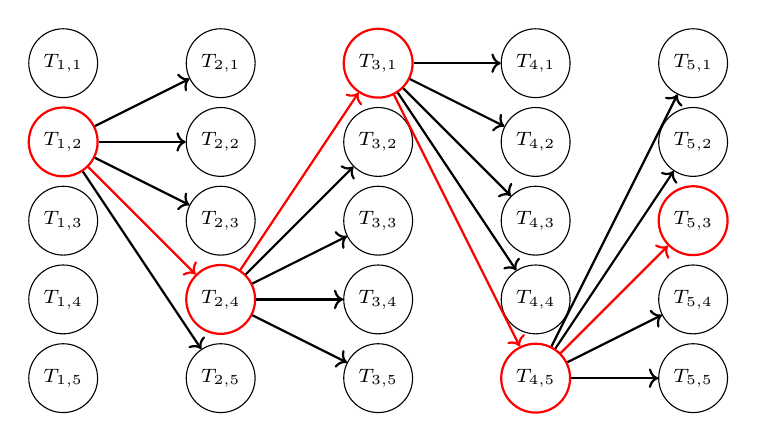
\begin{tikzpicture}[
  scale=1,
  every node/.style={
    circle,
    draw=black,
    fill=white,
    minimum size=0.8cm,
    font=\scriptsize
  },
  arrow/.style={->, thick},
  redarrow/.style={->, thick, red},
  redcircle/.style={circle, draw=red, thick, minimum size=0.8cm, font=\scriptsize}
]

% Node placement with explicit critical tasks
% Critical tasks: T_{1,2}, T_{2,4}, T_{3,1}, T_{4,5}, T_{5,3}

% Nodes for layer 1
\node (T11) at (0, 0) {$T_{1,1}$};
\node[redcircle] (T12) at (0, -1) {$T_{1,2}$};
\node (T13) at (0, -2) {$T_{1,3}$};
\node (T14) at (0, -3) {$T_{1,4}$};
\node (T15) at (0, -4) {$T_{1,5}$};

% Nodes for layer 2
\node (T21) at (2, 0) {$T_{2,1}$};
\node (T22) at (2, -1) {$T_{2,2}$};
\node (T23) at (2, -2) {$T_{2,3}$};
\node[redcircle] (T24) at (2, -3) {$T_{2,4}$};
\node (T25) at (2, -4) {$T_{2,5}$};

% Nodes for layer 3
\node[redcircle] (T31) at (4, 0) {$T_{3,1}$};
\node (T32) at (4, -1) {$T_{3,2}$};
\node (T33) at (4, -2) {$T_{3,3}$};
\node (T34) at (4, -3) {$T_{3,4}$};
\node (T35) at (4, -4) {$T_{3,5}$};

% Nodes for layer 4
\node (T41) at (6, 0) {$T_{4,1}$};
\node (T42) at (6, -1) {$T_{4,2}$};
\node (T43) at (6, -2) {$T_{4,3}$};
\node (T44) at (6, -3) {$T_{4,4}$};
\node[redcircle] (T45) at (6, -4) {$T_{4,5}$};

% Nodes for layer 5
\node (T51) at (8, 0) {$T_{5,1}$};
\node (T52) at (8, -1) {$T_{5,2}$};
\node[redcircle] (T53) at (8, -2) {$T_{5,3}$};
\node (T54) at (8, -3) {$T_{5,4}$};
\node (T55) at (8, -4) {$T_{5,5}$};
% Red critical path
\draw[redarrow] (T12) -- (T24);
\draw[redarrow] (T24) -- (T31);
\draw[redarrow] (T31) -- (T45);
\draw[redarrow] (T45) -- (T53);

% Black arrows from critical tasks to next layer (excluding red path edges)
\draw[arrow] (T12) -- (T21);
\draw[arrow] (T12) -- (T22);
\draw[arrow] (T12) -- (T23);
\draw[arrow] (T12) -- (T25);

\draw[arrow] (T24) -- (T32);
\draw[arrow] (T24) -- (T33);
\draw[arrow] (T24) -- (T34);
\draw[arrow] (T24) -- (T35);

\draw[arrow] (T31) -- (T41);
\draw[arrow] (T31) -- (T42);
\draw[arrow] (T31) -- (T43);
\draw[arrow] (T31) -- (T44);

\draw[arrow] (T45) -- (T51);
\draw[arrow] (T45) -- (T52);
\draw[arrow] (T45) -- (T54);
\draw[arrow] (T45) -- (T55);

\end{tikzpicture}
\caption{Lower-bound instance for \( P = 25 \), with 5 layers of 5 tasks. A single critical task per layer (circled in red) has successors in the next layer. Red arrows indicate the critical path formed across layers; all other tasks are independent.}
\label{fig:lower_bound_horizontal}
\end{figure}




To establish a fundamental lower bound, we construct an adversarial instance consisting of \( P = K^2 \) processors and \( n = P \) tasks, organized into \( \sqrt{P} \) layers of \( \sqrt{P} \) independent tasks each. Tasks are labeled \( \task_{i,j} \), where \( i \in \{1, \dots, \sqrt{P}\} \) denotes the layer index and \( j \in \{1, \dots, \sqrt{P}\} \) the position within the layer.

To introduce dependencies between layers, we designate one critical task per layer. Specifically, for each layer \( i \in \{1, \dots, \sqrt{P} - 1\} \), a single task \( \task_{i,j_i} \) is chosen to have successors: it precedes all tasks in the next layer \( i+1 \), while all other tasks in the layer remain independent. There are no additional precedence constraints.

This construction, illustrated in Figure~\ref{fig:lower_bound_horizontal}, is designed to model the behavior of an online adversary. Since all tasks in each layer appear identical upon release, the adversary can always pick the task that was completed last in layer \( i \) as the critical one \( \task_{i,j_i} \), thus enforcing dependencies after the fact and preventing the algorithm from advancing to layer \( i+1 \) until this specific task has completed.

For example, in Figure~\ref{fig:lower_bound_horizontal}, we suppose that the algorithm completes task \( T_{1,2} \) last in the first layer. The adversary then sets \( T_{1,2} \) as the critical task, making all tasks in layer 2 depend on it. The same logic applies in subsequent layers with tasks \( T_{2,4} \), \( T_{3,1} \), and \( T_{4,5} \).

This strategy ensures that the algorithm, regardless of its internal logic, is forced to process the layers sequentially—each layer must be fully processed before discovering the true critical task, which unlocks the next layer. In contrast, an optimal clairvoyant scheduler, aware of all dependencies and critical tasks in advance, would execute only the critical path (highlighted in red in the figure) using all processors, then process the remaining independent tasks in parallel. This large gap between the online and offline capabilities is what gives rise to the lower bound.


We assume a reasonable affine execution time model:
\[
t(p) = A - B(p - 1),
\]
meaning each additional processor reduces the execution time by a constant \( B \). We set the parameters so that \( t(1) = \sqrt{P} \) and \( t(P) = 1 \), yielding:
\[
A = \sqrt{P}, \quad B = \frac{\sqrt{P} - 1}{P - 1}.
\]

\begin{theorem}
\label{thm.lowerbound}
For this instance, any online algorithm has a competitive ratio of at least \( \frac{\sqrt{P}-1}{2} \).
\end{theorem}

\begin{proof}
Since all tasks appear identical when released, an online algorithm cannot distinguish the critical task in each layer. The adversary can thus ensure that the task \( \task_{i,j_i} \) finishes last within layer \( i \), delaying the availability of layer \( i+1 \).

We now analyze the minimum time needed to complete each layer under any algorithm. Two cases may occur:

\begin{itemize}
    \item \textbf{Case 1:} At least one task is allocated at most \( \sqrt{P} \) processors. Then its execution time is at least \( t(\sqrt{P}) \), which we compute explicitly:
    \[
    t(\sqrt{P}) = A - B(\sqrt{P} - 1) = \sqrt{P} - \frac{\sqrt{P} - 1}{P - 1} \cdot (\sqrt{P} - 1) \ge \sqrt{P} - 1.
    \]

    \item \textbf{Case 2:} All tasks receive more than \( \sqrt{P} \) processors. In this case, execution time is limited not by individual task durations, but by the total available work (area). Since area is increasing with processor count (by monotonicity), the total area of a layer is at least:
    \[
    \sqrt{P} \cdot a(\sqrt{P}) = \sqrt{P} \cdot \sqrt{P} \cdot t(\sqrt{P}) = P \cdot t(\sqrt{P}).
    \]
    Hence, even with full processor utilization, the layer takes at least:
    \[
    \frac{P \cdot t(\sqrt{P})}{P} = t(\sqrt{P}) \ge \sqrt{P} - 1.
    \]
\end{itemize}

In both cases, the completion time of each layer is at least \( \sqrt{P} - 1 \), and since there are \( \sqrt{P} \) layers, the total execution time satisfies:
\[
T \ge \sqrt{P} \cdot (\sqrt{P} - 1) = P - \sqrt{P}.
\]
Now consider a feasible offline schedule. It first executes the \( \sqrt{P} \) critical tasks \( \task_{i,j_i} \) sequentially using all \( P \) processors (each in time \( t(P) = 1 \)), for a total of \( \sqrt{P} \) time units. Then, the remaining \( P - \sqrt{P} \) tasks can be executed in parallel, each on a single processor, since there are at least \( P - \sqrt{P} \) available processors. These tasks have execution time \( t(1) = \sqrt{P} \), so the second phase takes at most \( \sqrt{P} \) time.

Hence, the total duration of the offline schedule is:
\[
T^{\opt} \le \sqrt{P} + \sqrt{P} = 2\sqrt{P}.
\]

Combining this with the earlier lower bound \( T \ge P - \sqrt{P} \), we obtain:
\[
\frac{T}{T^{\opt}} \ge \frac{P - \sqrt{P}}{2\sqrt{P}} =\frac{\sqrt{P}-1}{2}.
\]

\end{proof}



\section{Special Cases for Different Speedup Models}
\label{sec.anamodel}

\subsection{Deriving Competitive Ratios}

To derive a competitive ratio for a given speedup model, the idea is conceptually straightforward—considerably simpler than the constructions in \cite{ICPP22, TOPC24}.  
For each model~$M$, we determine the smallest constant $\ratio_M$ such that, for any task following the model, there exists a processor allocation $p$ satisfying
\[
\frac{t_j(p)}{t_j^{\min}} \le \ratio_M
\quad \text{and} \quad
\frac{a_j(p)}{a_j^{\min}} \le \ratio_M \,.
\]
We then substitute this value into the general bound from Lemma~\ref{lem.makespan}.  
Although the objective function differs from that of~\cite{TOPC24}, the approach is similar, and several previously derived results can be reused.

\begin{lemma}\label{lem.roofline}
For any task that follows the Roofline speedup model, there exists a processor allocation that achieves a ratio of at most $\ratio_{\ROO} = 1$.  
Therefore, \fair is $\frac{3 + \sqrt{5}}{2} <2.62$-competitive when all tasks follow the Roofline model.
\end{lemma}

\begin{proof}
This result is standard and follows easily.  
If a task~$j$ follows the Roofline model, its execution time is given by $t(p) = \frac{w}{\min(p, \bar{p})}$, where $w > 0$ and $\bar{p} \in \{1, \dots, P\}$.  
Setting the processor allocation to $p = \bar{p}$ yields the minimum execution time $t_j^{\min} = \frac{w}{\bar{p}}$.  
The corresponding area is $a_j(p) = p \cdot t(p) = w$ for all $p \le \bar{p}$, so the minimum area is $a_j^{\min} = w$.  
Hence, $\ratio_j(p) = 1$, and we conclude that $\ratio_{\ROO} = 1$.  
Plugging this into Equation~\eqref{eq.makespan} yields the claimed competitive ratio.
\end{proof}

\begin{remark}
The derived competitive ratio is tight in this setting; the proof is omitted for brevity.
\end{remark}

\begin{lemma}\label{lem.comm}
For any task that follows the communication model, there exists a processor allocation that achieves a ratio of at most  $\ratio_{\COM} = \sqrt{2}$.  
Therefore, \fair is $2 + \sqrt{2} < 3.42$-competitive when all tasks follow the communication model.
\end{lemma}

\begin{proof}
This proof is inspired by the analysis in \cite{TOPC24}.  
If a task $j$ follows the communication model, its execution time is given by
\[
t(p) = \frac{w}{p} + c(p - 1) = c\left( \frac{w'}{p} + p - 1 \right),
\]
with $w' > 0$ and $c > 0$.  
This function is decreasing on $[1, \sqrt{w'}]$ and increasing on $[\sqrt{w'}, \infty)$.

Let $p^{\max}$ denote the number of processors that minimizes the task’s execution time, i.e., $t(p^{\max}) = t^{\min}$.  
Clearly, either $p^{\max} = P$ or $\lfloor \sqrt{w'} \rfloor \le p^{\max} \le \lceil \sqrt{w'} \rceil$.  
Also, the minimum area is obtained with one processor: $a^{\min} = a(1) = c w'$.

Define \(f(w', p) = \frac{t(p)}{t^{\min}} = \frac{\frac{w'}{p} + p - 1}{\frac{w'}{p^{\max}} + p^{\max} - 1}\).  
We show that \(f(w', p)\) is non-decreasing with respect to \(w'\) in the interval \(w' \ge p^2\), by computing the partial derivative:
\begin{align*}
\frac{\partial f(w', p)}{\partial w'} &= 
\frac{
  \frac{1}{p}\left(\frac{w'}{p^{\max}} + p^{\max} - 1\right)
  - \frac{1}{p^{\max}}\left(\frac{w'}{p} + p - 1\right)
}{
  \left( \frac{w'}{p^{\max}} + p^{\max} - 1 \right)^2
} \\
&= 
\frac{
  \frac{p^{\max} - 1}{p} - \frac{p - 1}{p^{\max}}
}{
  \left( \frac{w'}{p^{\max}} + p^{\max} - 1 \right)^2
}.
\end{align*}
This is non-negative when \(p \le p^{\max}\), which is true for \(w' \ge p^2\). The continuity of $f$ is straightforward, hence it is non decreasing. We now consider four cases:

\textbf{Case 1:} \(w' \le 2 + 2\sqrt{2}\), set \(p = 1\).

\begin{align*}
\frac{a(p)}{a^{\min}}
      &= \frac{a(1)}{a(1)}
       = 1,\\[4pt]
\frac{t(p)}{t^{\min}}&=f(w',1) \leq f(2+2\sqrt{2},1)=\frac{2+2\sqrt{2}}{\frac{2+2\sqrt{2}}{2}+1} =\frac{2+2\sqrt{2}}{2+\sqrt{2}}=\frac{(2+2\sqrt{2})(2-\sqrt{2})}{2}=\sqrt{2},
\end{align*}

Indeed, for \(w' = 2 + 2\sqrt{2}\), \(p^{\max}=2\).

\textbf{Case 2:} \(2 + 2\sqrt{2} < w' \le 16\), set \(p = 2\).

\begin{align*}
\frac{a(p)}{a^{\min}} &=\frac{c(w'+2)}{cw'}=1+\frac{2}{w'} < 1+\frac{1}{1+\sqrt{2}}=1+\frac{\sqrt{2}-1}{(1+\sqrt{2})(\sqrt{2}-1)}=\sqrt{2}, \\[6pt]
\frac{t(p)}{t^{\min}}
      &= f(w',2)
       = \frac{\tfrac{w'}{2} + 1}{\tfrac{w'}{p^{\max}} + p^{\max} - 1}
       \le f(16,2)
       = \frac{\tfrac{16}{2} + 1}{\tfrac{16}{4} + 4 - 1}
       = \frac{9}{7}
       < \sqrt{2},
\end{align*}

Indeed, for \(w' = 16\), \(p^{\max}=4\).

\textbf{Case 3:} \(16 < w' \le 49\), set \(p = 3\).
\begin{align*}
\frac{a(p)}{a^{\min}}
      &= \frac{c\!\left(w' + p(p-1)\right)}{c w'}
       = 1 + \frac{6}{w'}
       \le 1 + \frac{6}{16}
       = \frac{22}{16}
       < \sqrt{2}, \\[6pt]
\frac{t(p)}{t^{\min}}
      &= f(w',3)
       = \frac{\tfrac{w'}{3} + 2}{\tfrac{w'}{p^{\max}} + p^{\max} - 1}
       \le f(49,3)
       = \frac{\tfrac{49}{3} + 2}{\tfrac{49}{7} + 7 - 1}
       = \frac{55}{39}
       < \sqrt{2},
\end{align*}

Indeed, for \(w' = 49\), \(p^{\max}=7\).


\textbf{Case 4:} \(w' > 49\).  
We use the lower bound \(t^{\min} \ge c(2\sqrt{w'} - 1)\) (attained by non-integer allocation), and set:
\(
p = \left\lfloor \sqrt{\frac{w'}{3}} + \frac{1}{2} \right\rfloor.
\)
This yields:
\begin{align*}
\frac{a(p)}{a^{\min}}&=\frac{c(w'+p(p-1))}{cw'}\leq 1+\frac{1}{w'}\left( \sqrt{\frac{w'}{3}}+\frac{1}{2}\right)\left(\sqrt{\frac{w'}{3}}-\frac{1}{2}\right)\leq 1+\frac{1}{w'}\frac{w'}{3} = \frac{4}{3}, \\[6pt]
\frac{t(p)}{t^{\min}} &\leq \frac{c\left(\frac{w'}{\sqrt{\frac{w'}{3}}-\frac{1}{2}} +\sqrt{\frac{w'}{3}}\right)}{c(2\sqrt{w'}-1)}= \frac{\left(\frac{\sqrt{w'}}{\frac{1}{\sqrt{3}}-\frac{1}{2\sqrt{w'}}} +\sqrt{\frac{w'}{3}}\right)}{(2\sqrt{w'}-1)}=\frac{1}{2-\frac{1}{\sqrt{w'}}}\left(\frac{1}{\frac{1}{\sqrt{3}}-\frac{1}{2\sqrt{w'}}} +\frac{1}{\sqrt{3}}\right).
\end{align*}

This function is decreasing in \(w'\), and using \(w' > 49\), we get:
\[
\frac{t(p)}{t^{\min}} \le \frac{1}{2 - \frac{1}{7}} \left( \frac{1}{\frac{1}{\sqrt{3}} - \frac{1}{14}} + \frac{1}{\sqrt{3}} \right) \approx 1.38 < \sqrt{2}.
\]

In all cases, we conclude that $\ratio_{\COM} = \sqrt{2}$, and substituting this into Equation~\ref{eq.makespan} gives:
\[
\frac{T}{T^{\opt}} = \frac{2\ratio_{\COM} + 1 + \sqrt{4\ratio_{\COM}^2 + 1}}{2} = \frac{2\sqrt{2} + 1 + \sqrt{9}}{2} = 2 + \sqrt{2}.
\]
\end{proof}

\begin{remark}
The derived competitive ratio is tight in this setting; the proof is omitted for brevity.
\end{remark}

\begin{lemma}\label{lem.amdahl}
For any task that follows the Amdahl speedup model, there exists a processor allocation that achieves a ratio of at most $\ratio_{\AMD}=2$. Therefore, \fair\ is $\frac{5+\sqrt{17}}{2} < 4.562$-competitive when all tasks follow the Amdahl model.
\end{lemma}

\begin{proof}
This result is well known and straightforward. If a task follows the Amdahl model, its execution time can be written $t(p)=\frac{w}{p}+d$, with $w>0$ and $d>0$. The minimum execution time satisfies $t^{\min}>d$, and the minimum area is obtained with just one processor, i.e., $a^{\min}=a(1)=w+d$.

We set $p=\min\!\bigl(\left\lceil \frac{w}{d} \right\rceil,\,P\bigr)$. Since $p\le\left\lceil \frac{w}{d} \right\rceil$, we have
\[
\frac{a(p)}{a^{\min}}
    =\frac{w+dp}{w+d}
    \le\frac{w+d\left(\frac{w}{d}+1\right)}{w+d}
    =\frac{w+d+w}{w+d}\le 2 .
\]
If $p=\left\lceil \tfrac{w}{d} \right\rceil$ (and thus $p\le P$), then
\[
\frac{t(p)}{t^{\min}}
    \le\frac{\frac{w}{\frac{w}{d}}+d}{d}
    \le 2 .
\]
Otherwise $p=P$, so $t(p)=t^{\min}$ and consequently $\tfrac{t(p)}{t^{\min}}=1<2$.

Hence this gives $\ratio_{\AMD}=2$, and substituting this value into Equation~\ref{eq.makespan} yields the desired competitive ratio.
\end{proof}

\begin{remark}
The derived competitive ratio is tight in this setting; the proof is omitted for brevity.
\end{remark}

\begin{lemma}\label{lem.general}
For any task that follows the General speedup model, there exists a processor allocation that achieves a ratio of at most $R^{\GEN}<2.018$. Therefore, \fair\ is $4.6$-competitive when all tasks follow the General model.
\end{lemma}

\begin{proof}
If a task follows the General model, its execution time can be written
$t(p) = \frac{w}{\min(p, \bar{p})} + d + c (p-1)
       = c\!\left( \frac{w'}{\min(p, \bar{p})} + d' + p - 1 \right)$,
with $w'>0$, $d'>0$, $c>0$, and $\bar{p}\ge 1$.
We distinguish two cases:

\textbf{Case 1:} $w' \le 800$.  
      Appendix~\ref{ap.general} shows that there exists a $p\in[1,8]$ such that
      $t(p)/t_{\min}\le 2.003$ and $a(p)/a_{\min}\le 2$.
      The proof proceeds by an exhaustive sub-case analysis; for example,
      if $w' \in [185,485]$ and $d' \in [80,170]$, the choice $p=3$ is valid.
      The detailed enumeration (13 subcases) is omitted here.

 \textbf{Case 2:} $w' > 800$.  
      Using a result from \cite{TOPC24}, choosing
      $p=\min\!\bigl(\lfloor \tfrac{w'+d'}{\sqrt{w'}+d'} + \tfrac12\rfloor,\bar{p}\bigr)$
      guarantees $t(p)/t_{\min}\le 2$ and
      $a(p)/a_{\min}\le \frac{1}{1-\frac{1}{2\sqrt{w'}}}+1$.
      The latter expression decreases with $w'$, and for $w'\ge 800$ we obtain
      $a(p)/a_{\min}<2.018$.


In all cases, the ratio is at most $R^{\GEN}<2.018$.
Plugging this into Equation~\ref{eq.makespan} shows that the competitive
ratio is below $4.6$.
\end{proof}

\begin{remark}
As with Amdahl, we believe that a sharper analysis would give
$R_{\GEN}=2$, in which case the derived competitive ratio would be identical
to that of Amdahl and thus tight in this setting.
\end{remark}

\begin{lemma}\label{lem.pcom}
For any task that follows the Power Communication model, there exists a processor allocation that achieves a ratio of at most $R^{\PCOM}<2.00424$. Therefore, \fair\ is $4.57$-competitive when all tasks follow the Power Communication model.
\end{lemma}

\begin{proof}
If a task follows the Power Communication model, its execution time can be written
$t(p) = \frac{w}{p} + c p^\gamma
       = c \left( \frac{w'}{p} + p^\gamma \right)$,
with $w'>0$ and $0<\gamma' \le 1$. Allowing $p$ to take non-integer values, a quick analysis shows that
the function $t(p)$ is minimised at
$p^{\star} = \left( \frac{w'}{\gamma} \right)^{\frac{1}{\gamma+1}}$; with
 $t_{min} \geq \left( \gamma+1\right)\left( \frac{w'}{\gamma} \right)^{\frac{\gamma}{\gamma+1}}$

We distinguish two cases:

\textbf{Case 1:} $w' \le 8$.  
Appendix~\ref{ap.powcom} shows that there exists a $p\in[1,8]$ such that
$t(p)/t_{\min}\le 2$ and $a(p)/a_{\min}\le 2$.
The proof proceeds by an exhaustive sub-case analysis; for example,
if $w' \in [3,4]$ and $\gamma\le 0.1$, choosing $p=4$ is valid.
The detailed enumeration (12 sub-cases) is omitted here.


\textbf{Case 2:} $w' \ge 8$ and $0\le\gamma\le 0.1$  
We set \(p=\left\lceil w'^{\frac{1}{\gamma+1}}\right\rceil\).  
Then  
\begin{align*}
\frac{t(p)}{t^{\min}} &= \frac{\frac{w'}{p}+p^\gamma}{t^{\min}} \le \frac{\frac{w'}{\,w'^{\frac{1}{\gamma+1}}} + \bigl(w'^{\frac{1}{\gamma+1}}+1\bigr)^\gamma}
        {(\gamma+1)\!\left(\frac{w'}{\gamma}\right)^{\frac{\gamma}{\gamma+1}}} \le \frac{w'^{\frac{\gamma}{\gamma+1}}
          + w'^{\frac{\gamma}{\gamma+1}}\!\left(1+\frac{1}{w'^{\frac{1}{\gamma+1}}}\right)^\gamma}
        {w'^{\frac{\gamma}{\gamma+1}}
          \bigl(\tfrac{\gamma+1}{\gamma^{\frac{\gamma}{\gamma+1}}}\bigr)} \\
&\le \frac{\gamma^{\frac{\gamma}{\gamma+1}}}{\gamma+1}
       \left(1+\left(1+\frac{1}{w'^{\frac{1}{\gamma+1}}}\right)^\gamma\right) \le \frac{1^{\frac{\gamma}{\gamma+1}}}{\gamma+1}
       \left(1+\bigl(1+1\bigr)^\gamma\right)
     = \frac{2^\gamma+1}{\gamma+1},
\end{align*}
and, because \(f(\gamma)=2^\gamma+1\) is convex while 
\(g(\gamma)=2(\gamma+1)\) is affine, with 
\(f(0)\le g(0)\) and \(f(0.1)\le g(0.1)\), we obtain
\(\frac{t(p)}{t^{\min}}\le 2.\)

\begin{align*}
\frac{a(p)}{a_{\min}} &= \frac{w'+p^{\gamma+1}}{w'+1}\le \frac{w'+\bigl(w'^{\frac{1}{\gamma+1}}+1\bigr)^{\gamma+1}}{w'+1}=   \frac{w'+w'\!\bigl(1+w'^{-\,\frac{1}{\gamma+1}}\bigr)^{\gamma+1}}{w'+1} \le \frac{w'+w'\!\bigl(1+w'^{-\,\frac{1}{1.1}}\bigr)^{1.1}}{w'+1}.
\end{align*}
Recall that for any real exponent $a$ and $|x|<1$ we have the generalized
binomial expansion
\[
(1+x)^a \;=\; \sum_{k=0}^{\infty} \binom{a}{k} x^{k},
\qquad
\binom{a}{k} = \frac{a(a-1)\cdots(a-k+1)}{k!}.
\]
When $1 < a < 2$ the first three coefficients are positive
($\binom{a}{0},\binom{a}{1},\binom{a}{2} > 0$),
whereas for every $k\ge 3$ the coefficients alternate in sign
and their absolute values decrease monotonically.
Hence the tail
\(
\sum_{k=3}^{\infty} \binom{a}{k} x^{k}
\)
is non-positive for $0 < x < 1$ (it starts with a negative term and the
remaining terms form an alternating series of diminishing magnitude).
Therefore truncating after the quadratic term provides an upper bound:
\[
\bigl(1+w'^{-\,\tfrac{1}{1.1}}\bigr)^{1.1}
   \;\le\;
   1 \;+\; 1.1\,w'^{-\,\tfrac{1}{1.1}}
   \;+\; 0.055\,w'^{-\,\tfrac{2}{1.1}}
   \;\le\;
   1 \;+\; 1.1\,w'^{-\,\tfrac{1}{1.1}}
   \;+\; 0.1\,w'^{-1}.
\]


Hence
\begin{align*}
\frac{a(p)}{a_{\min}} \le \frac{w'+w'\bigl(1+1.1\,w'^{-\,\frac{1}{1.1}}+0.1\,w'^{-1}\bigr)}{w'+1} \le \frac{2w'+1.1\,w'^{\frac{1}{11}}+0.1}{w'+1} =   2+\frac{\,1.1\,w'^{\frac{1}{11}}-1.9}{w'+1}.
\end{align*}

If \(w'\le \bigl(\tfrac{1.9}{1.1}\bigr)^{11}\) the fraction is non-positive,
so \(\frac{a(p)}{a_{\min}}\le 2\).
Otherwise,
\[
\frac{a(p)}{a_{\min}}
    \le 2+1.1\,w'^{-\,\frac{10}{11}}
    \le 2+\bigl(\tfrac{1.9}{1.1}\bigr)^{-10}
    < 2.00424.
\]

Thus, for all \(w'\ge 8\) and \(0\le\gamma\le0.1\),
\[
\frac{t(p)}{t^{\min}}\le 2
\quad\text{and}\quad
\frac{a(p)}{a_{\min}}<2.00424,
\]

\textbf{Case 3:}  $w' \ge 8$ and $\gamma > 0.1$.  
We set \(p=\bigl\lfloor w'^{\frac{1}{\gamma+1}}\bigr\rfloor\).

\begin{align*}
\frac{t(p)}{t^{\min}} = \frac{\tfrac{w'}{p}+p^\gamma}{t^{\min}} \le \frac{\displaystyle
              \frac{w'}{\,w'^{\frac{1}{\gamma+1}}-1}
              +\bigl(w'^{\frac{1}{\gamma+1}}\bigr)^{\gamma}}
            {(\gamma+1)\!\left(\frac{w'}{\gamma}\right)^{\frac{\gamma}{\gamma+1}}}= \frac{\gamma^{\frac{\gamma}{\gamma+1}}}{\gamma+1}
      \,\cdot\,
      \frac{\displaystyle
            \tfrac{w'^{\frac{\gamma}{\gamma+1}}}{1-w'^{-\frac{1}{\gamma+1}}}
            +w'^{\frac{\gamma}{\gamma+1}}}
           {w'^{\frac{\gamma}{\gamma+1}}} \le \frac{1}{\gamma+1}\!
      \left(\frac{1}{1-w'^{-\frac{1}{\gamma+1}}}+1\right).
\end{align*}

The right-hand side decreases with \(w'\), so we may replace \(w'\) with \(8\).  
The first factor that involves \(\gamma\) decreases with \(\gamma\), whereas the second increases.  
Define
\[
f(a,b)=\frac{1}{a+1}
        \left(
          \frac{1}{1-8^{-\frac{1}{b+1}}}+1
        \right).
\]
If \(a \le \gamma \le b\), then \(\tfrac{t(p)}{t^{\min}} \le f(a,b)\), because we upper-bound the decreasing factor by \(a\) and the increasing one by \(b\).  
A numerical evaluation gives
\[
f(0.1,0.15) < 2,\qquad
f(0.15,0.4) < 2,\qquad
f(0.4,1)   < 2,
\]
and therefore \(\frac{t(p)}{t^{\min}} < 2.\)

\medskip
\noindent
Finally,
\begin{align*}
\frac{a(p)}{a_{\min}}
   &= \frac{w'+p^{\gamma+1}}{w'+1} \le \frac{w'+\bigl(w'^{\frac{1}{\gamma+1}}\bigr)^{\gamma+1}}{w'+1}
   \le \frac{2w'}{w'+1} < 2 .
\end{align*}

\smallskip
\noindent
In all cases, \(R^{\PCOM}<2.00424\) yields a competitive ratio strictly below \(4.57\) when substituting in Equation~\ref{eq.makespan}.

\end{proof}

\begin{remark}
As with Amdahl, we believe that a sharper analysis would give
$R_{\PCOM}=2$, in which case the derived competitive ratio would match that
of Amdahl and be tight in this setting.
\end{remark}


We have derived competitive ratios for all considered speedup models, which are very close from the previous ones obtained with algorithms specific to the models, while ours is general. In the next subsection, we will discuss why those results are unlikely to be beatable, except with new groundbreaking techniques.

\subsection{Potential for Improvements}


To argue why further progress is unlikely without fundamentally new ideas, we first frame a broad family of algorithms.

\paragraph{The \textsc{LALIST} paradigm.}
We say that an algorithm belongs to \emph{Local-Allocation List Scheduling} (\textsc{LALIST}) when it satisfies two conditions:
\begin{enumerate}[label=(\roman*)]
    \item \textbf{Eager list scheduling.}  
          Whenever at least one task is ready and sufficient processors are idle, the algorithm schedules some ready task immediately.  The particular priority rule is irrelevant, but deliberate idling is forbidden.
    \item \textbf{Local processor allocation.}  
          The processor allocation chosen for a task depends only on that task’s speedup profile~$t(p)$.  Consequently, two identical tasks receive identical allocations, independent of the current system state or of other tasks in the queue.
\end{enumerate}

In the on-line setting our knowledge is inherently limited to the task that has
just been released; no information about yet-to-be-revealed successors is
available.
Consequently, papers such as \cite{ICPP22,TOPC24}  chose the
allocation of each task solely from that task’s speedup curve, exactly as
required by condition~(ii).
Once allocations are fixed, a greedy (ASAP) list scheduler seems to be the only
reasonable option, because any deliberate idling can be exploited by an
adversary to extend the makespan. It is the reason why condition~(i) was introduced.



When the entire DAG is known, all off-line algorithms follow a
\emph{two-phase approach}:
(1) analyse the full graph to assign a processor allocation to every task;
(2) run a greedy list schedule on those fixed allocations.\cite{Wang92_DAG,Chen13_concave, Lepere01_DAG, Jansen06_DAG}
While the allocations in Phase~(1) depend on global DAG properties for offline setting,
such data is not available online, hence the strongest condition of algorithm following the \textsc{LALIST} paradigm, where we assume tasks allocation only depend on their time function.

Intuitively, allowing the allocation to react to the instantaneous load might seem advantageous (e.g.\ ``use all processors if only one task is ready'').  Yet such state-dependent schemes can later regret that choice when a burst of new tasks arrives.  
Even in the off-line setting, where the entire DAG is known in advance, no state-adaptive allocation policy with a provably better ratio is known; in the on-line world the challenge is even harder.
For these reasons, only some new breakthrough ideas would lead to an algorithm that beats all heuristics belonging to \textsc{LALIST}, and we think such result is very unlikely to happen.


\renewcommand{\arraystretch}{1.7}
\begin{table*}[h]
\centering
\caption{Summary of parameters and competitive ratios for different speedup models (rounded down for the best possible bound, rounded up for our heuristics). In red are shown the tight bounds. }
\label{tab.all-values}
\begin{tabular}{| c | c | c | c | c |}
\hline
\textbf{Model $M$} & \cite{ICPP22} & \cite{TOPC24} & \fair & Lower Bound on Best \textsc{LALIST} Heuristic \\
\hline
Roofline (\ROO) & {\color{red} $2.62$} & {\color{red} $2.62$} & {\color{red} $2.62$} & $\frac{2}{3-\sqrt{5}} > 2.61$ \\
\hline
Comm. (\COM) & $3.61$ & {\color{red} $3.40$} & $3.41$ & $\frac{18}{23-\sqrt{313}} > 3.39$ \\
\hline
Amdahl (\AMD) & $4.74$ & {\color{red} $4.55$} & $4.56$ & $\frac{2}{1-\sqrt{8\sqrt{2}-11}} > 4.54$ \\
\hline
General (\GEN) & $5.72$ & $4.63 (4.58)^*$ & $4.6$ & $\frac{2}{1-\sqrt{8\sqrt{2}-11}} > 4.54$ \\
\hline
Extended COM (COM2) &  & $4.57^*$  & $4.57$ & $\frac{2}{1-\sqrt{8\sqrt{2}-11}} > 4.54$  \\
\hline
\end{tabular}
\end{table*}



\paragraph{Known limits of \textsc{LALIST}.}
In~\cite{TOPC24} the authors established tight lower bounds on the competitive ratio of any \textsc{LALIST} algorithm.  
For the Roofline, communication, and Amdahl models those bounds are met by algorithms specific model; as shown in Table~\ref{tab.all-values} \footnote{For the General Model, the Algorithm presented in \cite{TOPC24} actually achieves better bound than \fair, using the refined analysis, it can be shown to be $4.58$-competitive  Similarly, for Power Communication Model, we can easily derive a ratio of $4.57$} .  
No \textsc{LALIST} strategy—regardless of its priority rule—can do better.



\paragraph{Where \fair\ stands.}
Strictly speaking, \fair\ is not in \textsc{LALIST}, because each allocation also depends on the global ratio~$\rratio$ observed so far.  
However, a clairvoyant variant that is told in advance the model-dependent constant $\ratio^M$ could initialise $\rratio$ directly to~$\ratio^M$ instead of $1$ (the online to update is Line 2 in Algorithm~\ref{alg.online}).  
The analysis would then proceed unchanged, there would be no subsequent updates of $\rratio$ (and hence of~$\mu$), and the algorithm would belong to \textsc{LALIST}—achieving exactly the bounds of \fair shown in Table~\ref{tab.all-values}.

Thus the deviations of \fair\ from \textsc{LALIST} are not due to on-line state adaptation, but merely to learning each task’s speedup model on the fly.  
That \fair\ still comes within \(\le 1\%\) of the best possible ratios of a clairvoyant \textsc{LALIST} algorithm underscores how little room for improvement remains.


In summary, \fair almost matches the best algorithm that follows \textsc{LALIST} paradigm, even comparing to clairvoyant heuristics. To further improve the ratios, one would need techniques that break at least one of the condition  which would require some breakthrough ideas, for scheduling and for analysing.

%------------------------------------------------------------------
% Transition from theory to experiments
%------------------------------------------------------------------
\noindent
\textbf{From theory to practice.}
The preceding sections demonstrated that \fair\ is, in theory, within roughly
one percent of the best clairvoyant \textsc{LALIST} algorithms for every
speedup model we studied.
We now turn to an empirical validation: Section~\ref{sec.experiments} explains
how we generate workloads, which heuristics we test, and how we measure
performance.

%------------------------------------------------------------------
\section{Experiments}
\label{sec.experiments}
%------------------------------------------------------------------

We first describe the workloads (§\ref{sec:instance-gen}), then the
heuristics (§\ref{sec:heuristics}), and finally the experimental
protocol (§\ref{sec:exp-protocol}).

%------------------------------------------------------------------
\subsection{Instance Generation}
\label{sec:instance-gen}
%------------------------------------------------------------------
\paragraph{Task generation.}
Our study evaluates the scheduling heuristics on the five speedup models
defined in Section~\ref{sec.model}:
Roofline, communication, Amdahl, power-communication, and general.
For every instance each task is generated independently as follows:

\begin{itemize}
    \item \textbf{Total work} \(w_j\) — drawn in seconds from the
          task-generation framework; it equals \(t_j(1)\) for every model.
    \item \textbf{Parallelism bound} \(p_j^{\max}\) — uniform in $\,[1,512]$.
    \item \textbf{Sequential fraction ratio} $\rho_d$
          — log-uniform in $[10^{-3},10^{-0.5}]$
          (i.e.\ $\rho_d = 10^{\mathrm{Unif}(-3,-0.5)}$);  
          the absolute sequential part used in Amdahl-type terms is
          \(d_j = \rho_d \, w_j\).
    \item \textbf{Communication ratio} $\rho_c$
          — log-uniform in $[10^{-6},10^{-2}]$
          (i.e.\ $\rho_c = 10^{\mathrm{Unif}(-6,-2)}$);  
          the communication coefficient in the time functions is
          \(c_j = \rho_c \, w_j\).
    \item \textbf{Power exponent} $\gamma_j$ — uniform in $[0,1]$
          (only used in the power-communication model).
\end{itemize}

\noindent
Sampling $\rho_d$ and $\rho_c$ draws the
sequential part and the communication cost relative to each task’s
total work: a large task ($w_j$ high) is therefore more likely to carry a
proportionally larger sequential or communication component.



\paragraph{Graph generation.}
Task-dependency graphs are produced with \texttt{daggen},\footnote{Commit
\texttt{f3e8b6c} of
\url{https://github.com/frs69wq/daggen}.}
which creates synthetic DAGs organised in layers.
Edges connect a task in one layer to tasks in subsequent layers; if the
\textit{Jump} parameter exceeds~1, an edge may skip intermediate layers.

The following topology parameters control the structure of each graph:
\begin{itemize}
    \item \textbf{Density} $\in[0,1]$ (default $0.5$) — controls how many edges are created between consecutive layers.
          A value near $0$ yields a very sparse DAG (few dependencies,
          almost chain-like), whereas a value near $1$ produces a much denser
          graph with many inter-layer edges.
    \item \textbf{Fat} $\in[0,1]$ (default $0.5$) — width of the DAG.
          Low values create thin, chain-like graphs; high values yield
          wide, fork–join-like structures.
    \item \textbf{Regular} $\in[0,1]$ (default $0.5$) — uniformity of the task
          distribution across layers.
    \item \textbf{Jump} $\in[1,9]$ (default $5$) — maximum number of layers a
          dependency may skip, controlling the length of execution paths.
    \item \textbf{Number of tasks} $n\in[500,5000]$ (default $2500$).
    \item \textbf{Number of processors} $P\in[124,1024]$ (default $512$).
\end{itemize}

%------------------------------------------------------------------
\subsection{Heuristics}
\label{sec:heuristics}
%------------------------------------------------------------------

For every speedup model we compare five allocation policies:
\begin{itemize}
    \item \textbf{ICPP22} — heuristic presented in
          \cite{ICPP22} (labelled \emph{ICPP22} in all tables).
    \item \textbf{TOPC24} — heuristic presented in
          \cite{TOPC24} (labelled \emph{TOPC24}).
          \footnote{For the power-communication model we extend the
          allocation rules of both \cite{ICPP22} and \cite{TOPC24} using the
          analysis of Section~\ref{sec.anamodel}; the resulting variants follow
          the spirit of the original papers while remaining model-consistent.}
    \item \textbf{Fair} — our single, model-agnostic heuristic.
    \item \textbf{minTime} — allocate \(p_j=p_j^{\max}\), minimising each
          task’s execution time.
    \item \textbf{minArea} — allocate \(p_j=1\), minimising each
          task’s processor-time area.
\end{itemize}

These policies differ only in their processor-allocation rule.
They are orthogonal to the priority rule used to select which ready
task is launched next; we therefore evaluate four queue-ordering strategies:

\begin{itemize}
    \item \textbf{FIFO} (default) — first in, first out.
    \item \textbf{procs} — task requiring the largest allocation first.
    \item \textbf{area} — task with the largest area
          \(a(p)=t(p)\times p\) first.
    \item \textbf{length} — task with the largest execution time \(t(p)\) first
          (descending order).
\end{itemize}

%------------------------------------------------------------------
\subsection{Experimental Protocol}
\label{sec:exp-protocol}
%------------------------------------------------------------------





\begin{table}[ht]
    \centering
    \begin{tabular}{|l|l|l|l|l|}
        \hline
        \textbf{Param} & \textbf{Default} & \textbf{Test Values} & \textbf{Type} & \textbf{Description} \\ \hline
        $n$            & 2500             & [500,\,\dots,\,5000] & Scale   & Number of tasks \\ \hline
        $P$            & 512              & [124,\,\dots,\,1024] & System  & Available processors \\ \hline
        Priority       & FIFO             & [FIFO, procs\,\dots]       & Policy  & Queue-ordering strategy \\ \hline\hline
        Density        & 0.5              & [0,\,\dots,\,1]      & Graph   & Edge probability \\ \hline
        Fat            & 0.5              & [0,\,\dots,\,1]      & Graph   & Width/depth ratio \\ \hline
        Regular        & 0.5              & [0,\,\dots,\,1]      & Graph   & Degree uniformity \\ \hline
        Jump           & 5                & [1,\,\dots,\,9]      & Graph   & Maximum jump distance between layers \\ \hline
    \end{tabular}
    \caption{Experimental parameters and their default values.}
    \label{tab:exp-params}
\end{table}

For each speedup model and each parameter, we designed one experiment that
studies the impact of that parameter on heuristic quality.
All default settings and test ranges are summarised in
Table~\ref{tab:exp-params}.
For every speedup model and every parameter summarized in the table, we perform one experiment that isolates the impact
of that parameter on heuristic quality. To do so, we normalize the makespan by a simple lower bound on the best makespan achievable.

\paragraph{Practical lower bound.}
The analysis in Section~\ref{sec.analysis} compares each heuristic against the
optimal makespan \(T^{\opt}\), whose two classical components are
\(\tfrac{A^{\opt}}{P}\) (area bound) and \(C^{\opt}\) (critical-path bound).
Unfortunately, computing either \(A^{\opt}\) or the allocations that realise
\(C^{\opt}\) is NP-complete.%

For large-scale empirical comparisons we therefore use a
looser, polynomial Lower Bound:
\[
L \;=\;
\max\!\Bigl(\,
  \tfrac{A^{\min}}{P},\;
  C^{\min}
\Bigr),
\]
where
\[
A^{\min} \;=\;
\sum_{j=1}^{n} a_j(1),  \qquad
C^{\min} \;=\;
\max_{f}\;
\sum_{j\in f}\!
      t_j\!\bigl(p_j^{\max}\bigr).
\]
\begin{itemize}
  \item \(A^{\min}\) is the total area if every task runs on a single
        processor, which is the minimum possible area for the instance.
  \item \(C^{\min}\) is the length of the longest path when each task is
        executed with its allocation \(p_j^{\max}\) that minimises
        \(t_j(\,\cdot\,)\).
\end{itemize}
Both quantities are readily computable in \(O(|E|+|V|)\) time and clearly
satisfy \(A^{\min}\!\le A^{\opt}\) and \(C^{\min}\!\le C^{\opt}\), hence
\(L\le T^{\opt}\).  While \(L\) is less tight than the theoretical bound \footnote{%
  Polynomial‐time lower bounds tighter than the one we adopt do exist
  \cite{Lepere}, but evaluating them would largely dominate the runtime of the experiment.}, it
is sufficient for comparing heuristics and can be evaluated orders of
magnitude faster than solving—exactly or approximately—the optimal allocation
problem for every instance.

The experimental protocol is as follows:

\begin{enumerate}
    \item Set every parameter to its default value except the one under study,
          which is swept over all of its \textbf{Test Values}.
    \item For each setting, generate 50 random instances and simulate them with
          all heuristics.  
          The performance metric is the ratio \(\tfrac{T}{L}\), where \(L\) is
          a lower bound on the optimal makespan.
    \item Convert the 50 ratio values per heuristic into a box-plot.
          The box spans the 25th–75th percentiles; the horizontal black line
          marks the median; a star denotes the average.
          Whiskers extend to the 10th and 90th percentiles, and outliers
          beyond that range are shown as small circles.
    \item Produce two summary tables:  
          (i) the average ratio for each (heuristic, speedup model)
          pair plus the overall mean;  
          (ii) the worst ratio observed for each pair.
          Although, in principle, an empirical ratio could exceed the proven
          competitive guarantee (which compares to the true optimum), this
          never occurred; even after normalising by \(L\), all ratios remained
          below the theoretical limit.
\end{enumerate}

Complete numerical results and figures are provided in
Appendix~\ref{ap.experiments}.

\subsection{Summary of Results}

\begin{table}[htbp]
\centering
\caption{Average Values for Each Model and Heuristic}
\label{tab:average_values}
\begin{tabular}{lrrrrr}
\toprule
Model & ICPP22 & TOPC24 & Fair & minTime & minArea \\
Roofline & 1.28 & 1.28 & 1.28 & 1.52 & 11.28 \\
Communication & 1.75 & 1.38 & 1.38 & 2.97 & 10.22 \\
Amdahl & 2.32 & 1.98 & 2.01 & 21.31 & 7.88 \\
General & 2.74 & 1.50 & 1.60 & 4.86 & 5.37 \\
PowerCom & 1.52 & 1.46 & 1.35 & 2.84 & 12.76 \\
\midrule
Average & 1.92 & 1.52 & 1.52 & 6.70 & 9.50 \\
\bottomrule
\end{tabular}
\end{table}


\fair is as good as previous heuristics specific for each model
\section{Conclusion}
\label{sec.conclusion}

Great paper !


\appendix
\newpage

\section{Appendix : Proof that the models are monotonic}
\label{ap.detailedproof}

\begin{lemma}
All tasks belonging to speedup models introduced in this paper are monotonic on $[1, p_j^{\max}]$
\end{lemma}

\begin{proof}
Since Roofline, Communication and Amdahl model are all special case of the General Model, we only need to show the result for the General Model and the Extended Communication Model.
We must show that the given models satisfy the two conditions of the monotonic property:



\paragraph{1. General Model.}
Recall that for the General Model, the execution time is given by:
\[
t_j(p_j) = \frac{w_j}{\min(p_j, \bar{p}_j)} + d_j + c_j(p_j - 1)
\]

\textbf{Non-increasing execution time:}

For $p_j \leq \bar{p}_j$, we have:
\[
t_j(p_j) = \frac{w_j}{p_j} + d_j + c_j(p_j - 1)
\]
The derivative with respect to $p_j$ is:
\[
t_j'(p_j) = -\frac{w_j}{p_j^2} + c_j
\]

This derivative cancels when:
\[
p_j = \sqrt{\frac{w_j}{c_j}} \ .
\]

Let us define:
\[
p_j^{\max} = \arg\min_{p \in \left\{\left\lfloor \sqrt{\frac{w_j}{c_j}} \right\rfloor, \left\lceil \sqrt{\frac{w_j}{c_j}} \right\rceil\right\}} t_j(p)
\]
as the integer value that minimizes $t_j(p)$ among the two integers closest to the real-valued optimum.

We distinguish two cases:

- If $\min(P, \bar{p}_j) \leq p_j^{\max}$, then the execution time strictly decreases on $[1, \min(P, \bar{p}_j)]$, and the minimum is attained at $p_j^{\max} = \min(P, \bar{p}_j)$.

- Otherwise, $t_j(p)$ decreases until $p_j^{\max}$ and increases afterward. Thus, the execution time is non-increasing on $[1, p_j^{\max}]$, where $p_j^{\max} = \min\left(p_j^{\max}, \bar{p}_j, P\right)$.

Therefore, the execution time is non-increasing on $[1, p_j^{\max}]$.

\textbf{Non-decreasing area:}

The area is defined by $a_j(p_j) = p_j \cdot t_j(p_j)$.

For $p_j \leq \bar{p}_j$:
\[
a_j(p_j) = p_j \left( \frac{w_j}{p_j} + d_j + c_j(p_j - 1) \right) = w_j + p_j d_j + c_j p_j(p_j - 1)
\]

The derivative is:
\[
a_j'(p_j) = d_j + c_j(2p_j - 1)
\]
With $c_j \geq 0$ and $p_j \geq 1$, this derivative is always non-negative, so $a_j(p_j)$ is non-decreasing on $[1, \bar{p}_j]$.

For $p_j > \bar{p}_j$, recall that $t_j(p_j)$ increases linearly, so:
\[
a_j(p_j) = p_j \cdot \left( \frac{w_j}{\bar{p}_j} + d_j + c_j(p_j - 1) \right)
\]
which is also strictly increasing as it is a convex quadratic function. Thus, $a_j(p_j)$ is non-decreasing on the whole domain.

Hence, the General Model satisfies both monotonic conditions.

\paragraph{2. Power communication model}

Recall the execution-time expression
\[
t_j(p_j)\;=\;\frac{w_j}{p_j}\;+\;c_j\,p_j^{\gamma_j},
\qquad
w_j>0,\; c_j>0,\; 0<\gamma_j\le 1.
\]

\subparagraph*{Shape of the execution-time curve.}
Our goal is to show that \(t_j(p_j)\) is either monotonically increasing, or it first decreases and then increases, as the processor allocation \(p_j\) grows.

Taking the derivative gives
\[
t_j'(p_j)\;=\;-\frac{w_j}{p_j^{2}}\;+\;c_j\gamma_j\,p_j^{\gamma_j-1}.
\]
Multiplying by \(p_j^{2}\) (strictly positive) lets us track the sign more easily:
\[
g(p_j)\;=\;p_j^{2}t_j'(p_j)\;=\;-\,w_j\;+\;c_j\gamma_j\,p_j^{\gamma_j+1}.
\]
Hence, \(\operatorname{sign}\bigl(t_j'(p_j)\bigr)=\operatorname{sign}\bigl(g(p_j)\bigr)\).

\medskip
Key properties of \(g\).
\begin{itemize}
  \item At \(p_j=1\): \(g(1)=c_j\gamma_j-w_j\).
  \item As \(p_j\to\infty\): \(g(p_j)\to\infty\) because \(\gamma_j+1>0\).
  \item Derivative: \(g'(p_j)=c_j\gamma_j(\gamma_j+1)\,p_j^{\gamma_j}>0\); hence \(g\) is strictly increasing.
\end{itemize}

Two regimes follow.

\begin{enumerate}
\item \textbf{Always-increasing time (\(c_j\gamma_j\ge w_j\)).}\\
      When \(g(1)\ge 0\), monotonicity of \(g\) implies \(g(p_j)\ge 0\) for every \(p_j\ge 1\).
      Consequently \(t_j'(p_j)\ge 0\) and \(t_j(p_j)\) grows with the processor allocation.

\item \textbf{Decrease-then-increase (\(c_j\gamma_j< w_j\)).}\\
      Here \(g(1)<0\) but \(g(p_j)\) eventually becomes positive.
      Because \(g\) is continuous and strictly increasing, there exists a unique
      \[
      p_j^{\ast}>1\quad\text{such that}\quad g(p_j^{\ast})=0 .
      \]
\end{enumerate}

      Thus, \( t_j(p_j) \) either increases or decreases then increases over \( p_j \geq 
p_j^{\max} = \arg\min_{p \in \left\{\left\lfloor p_j^* \right\rfloor, \left\lceil p_j^* \right\rceil\right\}} t_j(p)
\).

\subparagraph*{Monotonicity of the area.}
The processor-time area is
\[
a_j(p_j)\;=\;p_j\,t_j(p_j)
            \;=\;w_j\;+\;c_j\,p_j^{\gamma_j+1}.
\]
Differentiating,
\[
a_j'(p_j)
    \;=\;c_j(1+\gamma_j)\,p_j^{\gamma_j}\;\ge\;0,
\]
because \(c_j>0\) and \(\gamma_j\ge 0\).
Hence the area is monotone non-decreasing in the processor allocation, as required.

\end{proof}



\section{Appendix : Complete Proof of General ratio}
\label{ap.general}


\begin{lemma}
For any task that follows the General speedup model, there exists a processor allocation that achieves a ratio no greater than $R^{\GEN}<2.018$. Consequently, \fair\ is $4.6$-competitive when all tasks follow the General model.
\end{lemma}

\begin{proof}
If a task follows the General model, its execution time can be written
\[
t(p)=\frac{w}{\min(p,\bar p)}+d+c(p-1)
     =c\!\left(\frac{w'}{\min(p,\bar p)}+d'+p-1\right),
\]
with $w'>0$, $d'>0$, $c>0$, and $\bar p\ge1$.
Allowing $p$ to take non-integer values and assuming $\bar p$ is unbounded,
the function $t(p)$ is minimised at
$p^{\star}=\sqrt{w'}$; hence
\[
t^{\min}\;\ge\;c\bigl(2\sqrt{w'}+d'-1\bigr).
\]
(The bound also holds when $\bar p<p^{\star}$, since then the minimum occurs
at $p=\bar p$ and is even larger.)
The minimum area is obtained with one processor:
$a^{\min}=a(1)=c(w'+d')$.

Let $p^{\max}$ denote the (integer) processor count that minimises the
execution time, i.e.\ $t(p^{\max})=t^{\min}$.  
Either $p^{\max}=\bar p$ or
$\lfloor\sqrt{w'}\rfloor\le p^{\max}\le\lceil\sqrt{w'}\rceil$.

We analyse four cases.

\textbf{Case 1:} $w'\le4$ or $\bar p=1$.  
Then $p^{\max}\le2$; setting $p=1$ yields
\[
\frac{a(p)}{a^{\min}}=1,
\qquad
\frac{t(p)}{t^{\min}}\le2.
\]

\textbf{Case 2:} $4<w'\le800$ and $d'>800$.  
Choosing $p=1$ gives $t^{\min}>d'>w'$ and
$t(1)=w+d<2\,t^{\min}$.


\begin{figure}[ht]
    \centering
    \begin{subfigure}{0.32\textwidth}
        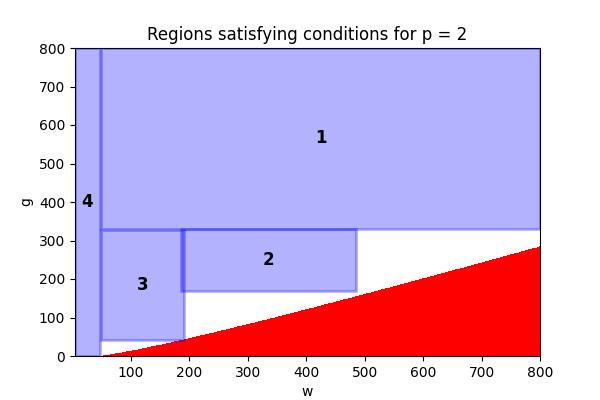
\includegraphics[width=\linewidth]{plotsgen/plot_p_2.png}
        \caption{$p = 2$}
    \end{subfigure}
    \hfill
    \begin{subfigure}{0.32\textwidth}
        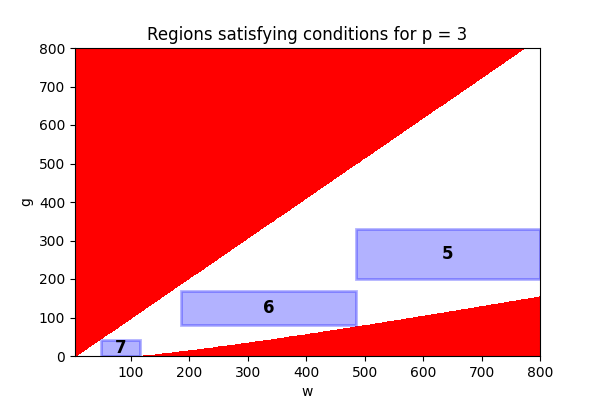
\includegraphics[width=\linewidth]{plotsgen/plot_p_3.png}
        \caption{$p = 3$}
    \end{subfigure}
    \hfill
    \begin{subfigure}{0.32\textwidth}
        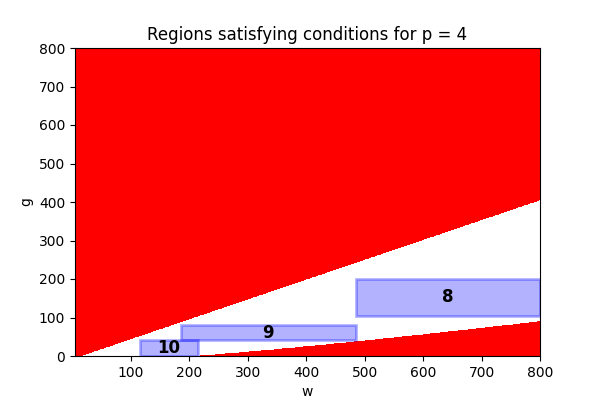
\includegraphics[width=\linewidth]{plotsgen/plot_p_4.png}
        \caption{$p = 4$}
    \end{subfigure}
    \hfill
    \begin{subfigure}{0.32\textwidth}
        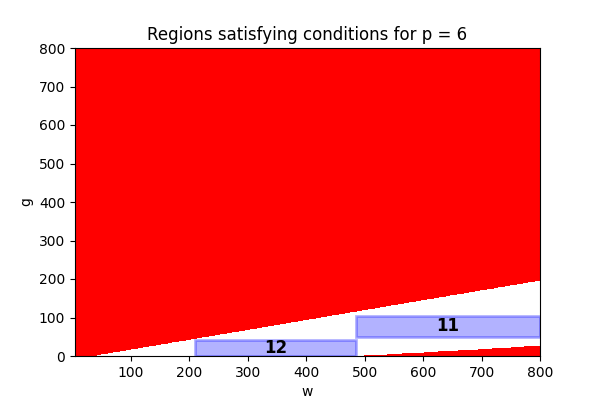
\includegraphics[width=\linewidth]{plotsgen/plot_p_6.png}
        \caption{$p = 6$}
    \end{subfigure}
    \hfill
    \begin{subfigure}{0.32\textwidth}
        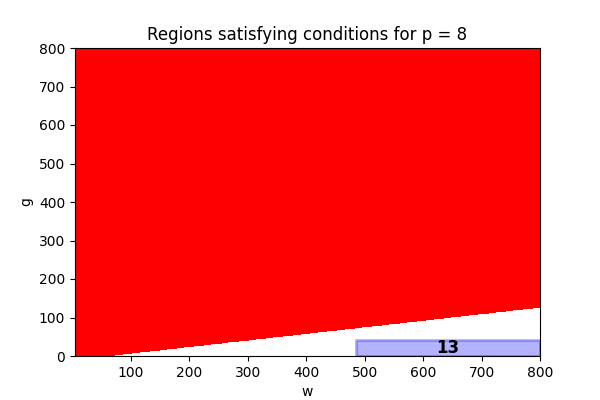
\includegraphics[width=\linewidth]{plotsgen/plot_p_8.png}
        \caption{$p = 8$}
    \end{subfigure}
    \begin{subfigure}{0.32\textwidth}
        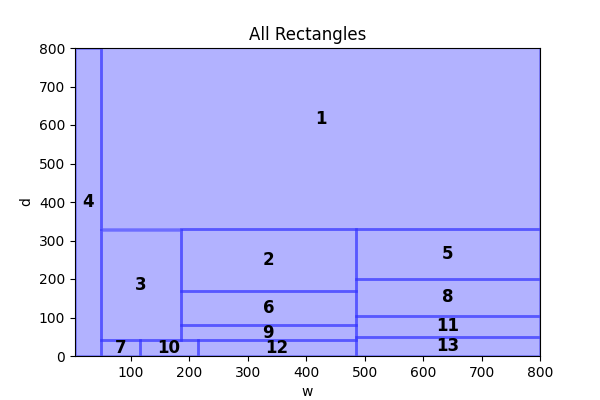
\includegraphics[width=\linewidth]{plotsgen/rectanglesall.png}
        \caption{all rectangles}
    \end{subfigure}
    \caption{Comparative plots for different values of $p$.}
    \label{fig:all_plotsgen}
\end{figure}

\begin{figure}
\center
\begin{tabular}{|c|c|c|c|c|c|c|}
\hline
Rectangle & $(w_1,\gamma_1)$ & $(w_2,\gamma_2)$ & $p$ & $p_{min}(w_1,\gamma_1,p) $& $f(w_1,\gamma_1,p)$ & $g(w_2,\gamma_2,p)$ \\
\hline
1 & $(49,800)$ & $(800,330)$ & 2 &7 & 1.94 & 1.90 \\
2 & $(185,330)$ & $(485,170)$ & 2 &14 & 1.64 & 1.94 \\
3 & $(49,330)$ & $(185,42)$ & 2 &7 & 1.88 & 1.99 \\
4 & $(4,800)$ & $(49,0)$ & 2 &2 & 2.00 & 1.96 \\
5 & $(485,330)$ & $(800,200)$ & 3 &22 & 1.82 & 1.83 \\
6 & $(185,170)$ & $(485,80)$ & 3 &14 & 1.97 & 1.98 \\
7 & $(49,42)$ & $(115,0)$ & 3 &7 & 1.99 & 1.97 \\
8 & $(485,200)$ & $(800,105)$ & 4 &22 & 1.89 & 1.92 \\
9 & $(185,80)$ & $(485,42)$ & 4 &14 & 1.95 & 1.95 \\
10 & $(115,42)$ & $(210,0)$ & 4 &11 & 1.88 & 1.98 \\
11 & $(485,105)$ & $(800,50)$ & 6 &22 & 1.94 & 1.78 \\
12 & $(210,42)$ & $(485,0)$ & 6 &14 & 1.95 & 1.99 \\
13 & $(485,50)$ & $(800,0)$ & 8 &22 & 1.76 & 1.93 \\
\hline
\end{tabular}
\caption{Verification of all extreme values in sub-areas}
\label{fig.verif2}
\end{figure}
\textbf{Case 3}: We first assume that $\bar{p}$ is unbounded.  
Define
\[
\alpha(w',d',p)=\frac{a(w',d',p)}{a_{\min}(w',d')}
               =\frac{w'+pd'+p(p-1)}{w'+d'}
               =1+\frac{(p-1)(d'+p)}{w'+d'} .
\]
The function $\alpha(w',d',p)$ is decreasing in $w'$.  
Differentiating with respect to $d'$ gives
\[
\frac{\partial\alpha(w',d',p)}{\partial d'}
   =\frac{(w'-p)(p-1)}{(w'+d')^{2}}>0
   \quad\text{whenever } w'>p .
\]

Next, set
\[
\beta(w',d',p)=\frac{t(w',d',p)}{t_{\min}(w',d')}
             \ge\frac{\tfrac{w'}{p}+d'+p-1}{
                     \tfrac{w'}{p^{\max}}+d'+p^{\max}-1},
\]
for any $p^{\max}\ge p$.  
With $p$ fixed and $p<p^{\max}$, the ratio \(\beta\) increases with $w'$ (a
larger~$w'$ implies more parallel work and thus a larger
$\tfrac{t}{t_{\min}}$) and decreases with $d'$ for the exact same reason as long as $p<p^{\max}$.  
This can be verified formally and is omitted here for brevity.  
Finally, note that $p^{\max}$ itself naturally increases with $w'$ (more parallelism) and decreases with
$d'$ (less parallelism).

Therefore, suppose we are given a pair $(w',d')$ such that  
$w_{1}\le w'\le w_{2}$, $d_{2}\le d'\le d_{1}$, and a value $p$ satisfying  
$p^{\max}(w_{1},d_{1})\ge p$, 
$\alpha(w_{1},d_{1},p)\le2$, and $\beta(w_{2},d_{2},p)\le2$. 

Then $\alpha(w',d',p)\le2$ and $\beta(w',d',p)\le2$ for the entire rectangle
$\bigl[w_{1},w_{2}\bigr]\times\bigl[d_{2},d_{1}\bigr]$.

Figure~\ref{fig:all_plots} illustrates this idea.  
For each $p\in\{2,3,4,6,8\}$ we colour in red the regions where
$\alpha(w',d',p)>2$ (upper-left) and where $\beta(w',d',p)>2$
(lower-right), using a Python script.  
We then subdivide the domain $(w'\in[4,800],\,d'\in[0,800])$ into
13 sub-rectangles, assigning a single value of $p$ to each; for example,
sub-rectangle~5 uses $p=3$.  
To confirm that a sub-rectangle avoids the red zones without relying on the
script, it suffices to check:
\begin{itemize}
    \item the upper-left corner for $\alpha$: $\alpha(w_{1},d_{1},p)\le2$,
    \item the lower-right corner for $\beta$: $\beta(w_{2},d_{2},p)\le2$,
    \item that $p \le p^{\max}$ at the upper-left corner: $p^{\max}(w_{1},d_{1})\ge p$,
    \item and that $p^2 \le w_1$.
\end{itemize}


All of these checks are summarised in the table in
Figure~\ref{fig.verif2}.

\medskip
We have thus shown that, when $\bar{p}$ is unbounded, there exists a
processor count $p'$ such that
\(\tfrac{t(p')}{t_{min}}\le2.018\) and
\(\tfrac{a(p')}{a_{min}}\le2.018\).
If instead $\bar{p}<p'$, we simply set $p=\bar{p}=p^{\max}$; this choice
reduces the area and yields $t(p)=t_{min}$.

\textbf{Case 4:} $w'>800$.  
This case is treated in the main body of the paper.

\medskip
In every case the ratio is bounded by $R^{\GEN}<2.018$.
Substituting this value into Equation~\eqref{eq.makespan}
gives a competitive ratio strictly below $4.6$.
\end{proof}


\FloatBarrier 
\newpage
\section{Appendix : Complete Proof of Extended Communication ratio}
\label{ap.powcom}
\begin{lemma}\label{lem.pcom}
For any task that follows the Power Communication model, there exists a processor allocation that achieves a ratio of at most $R^{\PCOM}<2.00424$. Therefore, \fair\ is $4.566$-competitive when all tasks follow the Power Communication model.
\end{lemma}

\begin{proof}
If a task follows the Power Communication model, its execution time can be written
$t(p) = \frac{w}{p} + c p^\gamma
       = c \left( \frac{w'}{p} + p^\gamma \right)$,
with $w'>0$ and $0<\gamma \le 1$.  Allowing $p$ to take non-integer values, a quick analysis shows that
the function $t(p)$ is minimised at
$p^{\star} = \left( \frac{w'}{\gamma} \right)^{\frac{1}{\gamma+1}}$; with
 $t_{min} \geq \left( \gamma+1\right)\left( \frac{w'}{\gamma} \right)^{\frac{\gamma}{\gamma+1}}$.

\textbf{Case 1}: $w \leq 2$.  
If $p^{\max}=1$, then we choose $p=1$ and get $\frac{a(p)}{a_{\min}} = \frac{t(p)}{t_{\min}} = 1$. Otherwise, we choose $p=2$. Since $t(2) \leq t(1)$, we have $a(2) \leq 2a_{\min}$. Finally, $t(2) = c\left(\frac{w'}{2} + 2^\gamma \right) \leq c(1 + 2^\gamma) \leq c\left(1 + ({p^{\max}})^\gamma \right) \leq c +t_{\min}$. Since $t_{\min} \geq c$, we have $\frac{t(p)}{t_{\min}} \leq 2$.

\begin{figure}[ht]
    \centering
    \begin{subfigure}{0.32\textwidth}
        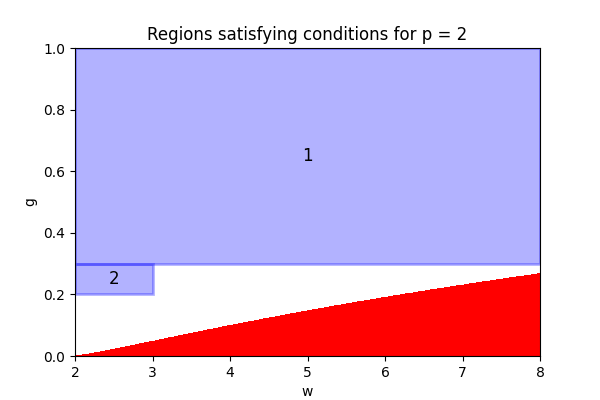
\includegraphics[width=\linewidth]{plotsexcom/plot_p_2.png}
        \caption{$p = 2$}
    \end{subfigure}
    \hfill
    \begin{subfigure}{0.32\textwidth}
        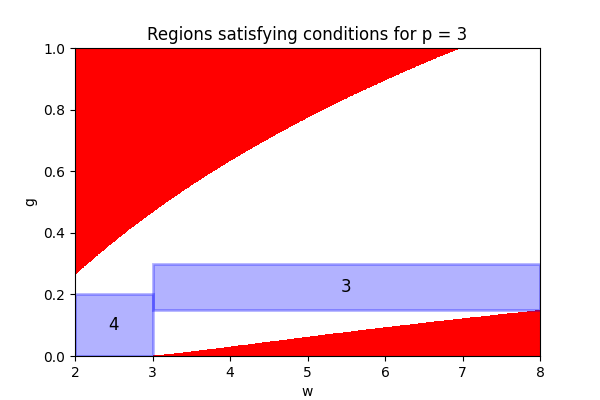
\includegraphics[width=\linewidth]{plotsexcom/plot_p_3.png}
        \caption{$p = 3$}
    \end{subfigure}
    \hfill
    \begin{subfigure}{0.32\textwidth}
        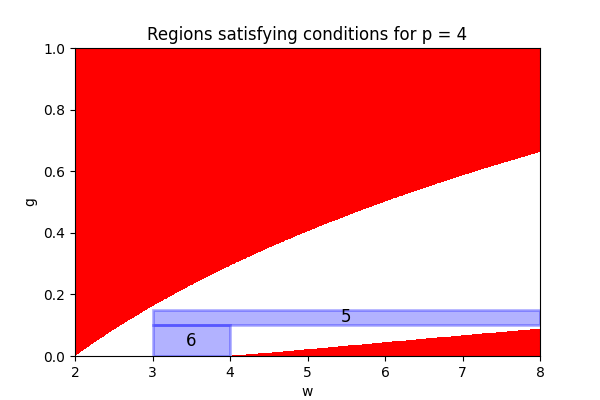
\includegraphics[width=\linewidth]{plotsexcom/plot_p_4.png}
        \caption{$p = 4$}
    \end{subfigure}
    \hfill
    \begin{subfigure}{0.32\textwidth}
       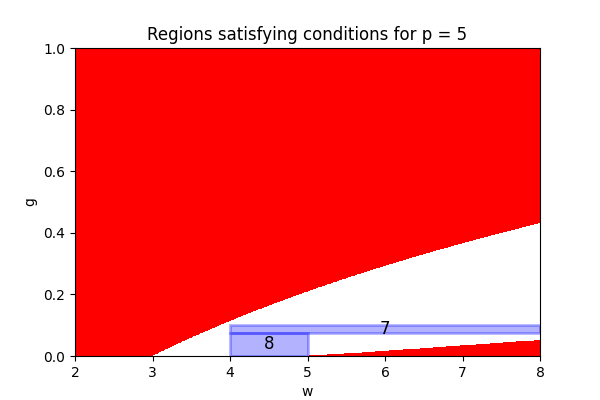
\includegraphics[width=\linewidth]{plotsexcom/plot_p_5.png}
        \caption{$p = 5$}
    \end{subfigure}
    \medskip
    \begin{subfigure}{0.32\textwidth}
        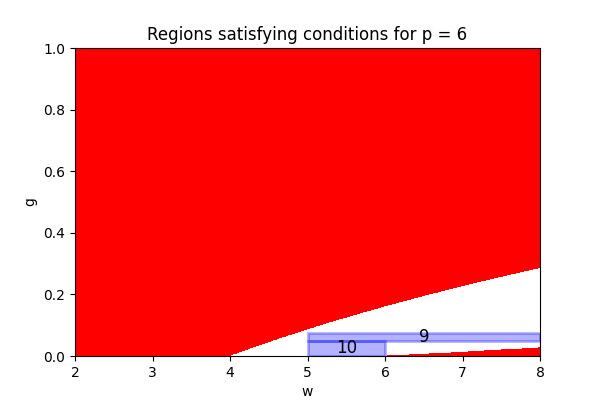
\includegraphics[width=\linewidth]{plotsexcom/plot_p_6.png}
        \caption{$p = 6$}
    \end{subfigure}
    \hfill
    \begin{subfigure}{0.32\textwidth}
        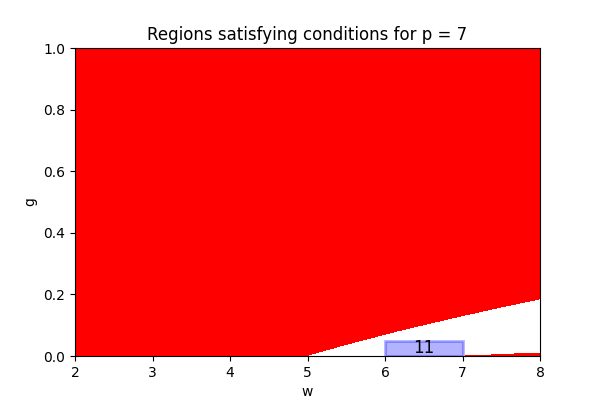
\includegraphics[width=\linewidth]{plotsexcom/plot_p_7.png}
        \caption{$p = 7$}
    \end{subfigure}
    \hfill
    \begin{subfigure}{0.32\textwidth}
        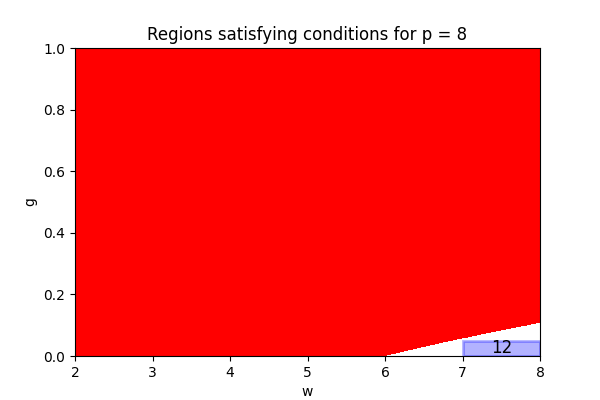
\includegraphics[width=\linewidth]{plotsexcom/plot_p_8.png}
        \caption{$p = 8$}
    \end{subfigure}
    \begin{subfigure}{0.32\textwidth}
        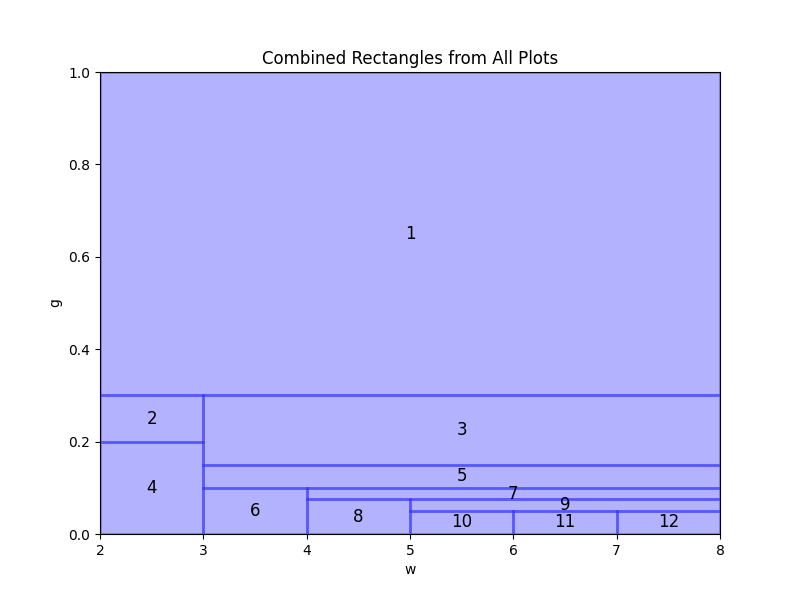
\includegraphics[width=\linewidth]{plotsexcom/rectanglesall.png}
        \caption{all rectangles}
    \end{subfigure}
    \caption{Comparative plots for different values of $p$.}
    \label{fig:all_plots}
\end{figure}

\begin{figure}
\center
\begin{tabular}{|c|c|c|c|c|c|c|}
\hline
Rectangle & $(w_1,\gamma_1)$ & $(w_2,\gamma_2)$ & $p$ & $p_{\max}(w_1,\gamma_1,p) $& $\alpha(w_1,\gamma_1,p)$ & $\beta(w_2,\gamma_2,p)$ \\
\hline
1 & $(2,1)$ & $(8,0.3)$ & 2 &1 & 2.00 & 1.89 \\
2 & $(2,0.3)$ & $(3,0.2)$ & 2 &4 & 1.49 & 1.41 \\
3 & $(3,0.3)$ & $(8,0.15)$ & 3 &6 & 1.79 & 1.99 \\
4 & $(2,0.2)$ & $(3,0)$ & 3 &7 & 1.91 & 2.00 \\
5 & $(3,0.15)$ & $(8,0.1)$ & 4 &14 & 1.98 & 1.92 \\
6 & $(3,0.1)$ & $(4,0)$ & 4 &22 & 1.90 & 2.00 \\
7 & $(4,0.1)$ & $(8,0.075)$ & 5 &29 & 1.97 & 1.83 \\
8 & $(4,0.075)$ & $(5,0)$ & 5 &40 & 1.93 & 2.00 \\
9 & $(5,0.075)$ & $(8,0.05)$ & 6 &50 & 1.98 & 1.82 \\
10 & $(5,0.05)$ & $(6,0)$ & 6 &80 & 1.93 & 2.00 \\
11 & $(6,0.05)$ & $(7,0)$ & 7 &96 & 1.96 & 2.00 \\
12 & $(7,0.05)$ & $(8,0)$ & 8 &111 & 1.98 & 2.00 \\
\hline
\end{tabular}
\label{fig.verif}
\caption{Verification of all extreme values in sub-areas}
\end{figure}\textbf{Case 2}: $2 \leq w' < 8$.  
Let  $\alpha(w',\gamma,p)= \frac{a(w',\gamma,p)}{a_{\min}(\gamma,p)} = \frac{w' + p^{\gamma+1}}{w' + 1}$ and $\beta(w',\gamma,p) = \frac{t(w',\gamma,p)}{t_{\min}(\gamma,p)} = \frac{\frac{w'}{p} + p^\gamma}{\frac{w'}{p^{\max}} + {p^{\max}}^\gamma}$. The objective is to show that for any pair $(w',\gamma)$, there exists a $p$ such that $\alpha(w',\gamma,p) \leq 2$ and $\beta(w',\gamma,p) \leq 2$.

We observe that $\alpha(w',\gamma,p) = 1 + \frac{p^{\gamma+1} - 1}{w' + 1}$ increases with $\gamma$ and decreases with $w'$.  
Similarly, if $p^{\max} \geq p$, with $p$ fixed and $p < p^{\max}$, the ratio $\beta(w',\gamma,p)$ increases with $w'$ (a larger $w'$ implies more parallel work and thus a larger $\frac{t}{t_{\min}}$) and decreases with $\gamma$ (since a higher communication cost implies less efficient parallelism).  
Additionally, $p^{\max}$ increases with $w'$ (more parallelism) and decreases with $\gamma$ (less parallelism), assuming all other parameters are fixed. This can be verified via a quick analysis, omitted here.

Therefore, if for a pair $(w',\gamma)$ we are given $w_1 \leq w' \leq w_2$, $\gamma_2 \leq \gamma \leq \gamma_1$, and a $p$ such that $p^{\max}(w_1,\gamma_1) \geq p$, $\alpha(w_1,\gamma_1,p) \leq 2$, and $\beta(w_2,\gamma_2,p) \leq 2$, then we are assured that $\alpha(w',\gamma,p) \leq 2$ and $\beta(w',\gamma,p) \leq 2$.

We further illustrate this with Figure~\ref{fig:all_plots}: for each $p \in [2,8]$, we color in red the areas where $\alpha(w',\gamma,p) > 2$ (top-left area) and where $\beta(w',\gamma,p) > 2$ (bottom-right area). We subdivide the region $(w' \in [2,8],\; \gamma \in [0,1])$ into 13 subrectangles, each assigned a single value of $p$. For instance, rectangle 3 is assigned $p = 3$. To confirm that a sub-rectangle avoids the red zones without relying on the
script, it suffices to check:
\begin{itemize}
    \item the upper-left corner for $\alpha$: $\alpha(w_1, \gamma_1, p) \leq 2$,
    \item the lower-right corner for $\beta$: $\beta(w_2, \gamma_2, p) \leq 2$,
    \item that $p \leq p^{\max}$ at the upper-left corner: $p^{\max}(w_1, \gamma_1) \geq p$,
\end{itemize}

All these checks are summarized in the table in Figure~\ref{fig.verif2} (note that the values are rounded, but the entries marked $2.00$ are exactly 2).

\textbf{Case 3}: $w' > 8$.  
This case is treated in the main body of the paper.

\smallskip
\noindent
In all cases, we conclude that \(R^{\PCOM}<2.00424\), which yields a competitive ratio strictly below \(4.57\) when substituted into Equation~\ref{eq.makespan}.
\end{proof}


\FloatBarrier 
\newpage
\section{Appendix : Full Experimental Results}
\label{ap.experiments}


\begin{figure}[htbp]
\centering
\begin{subfigure}[b]{0.32\textwidth}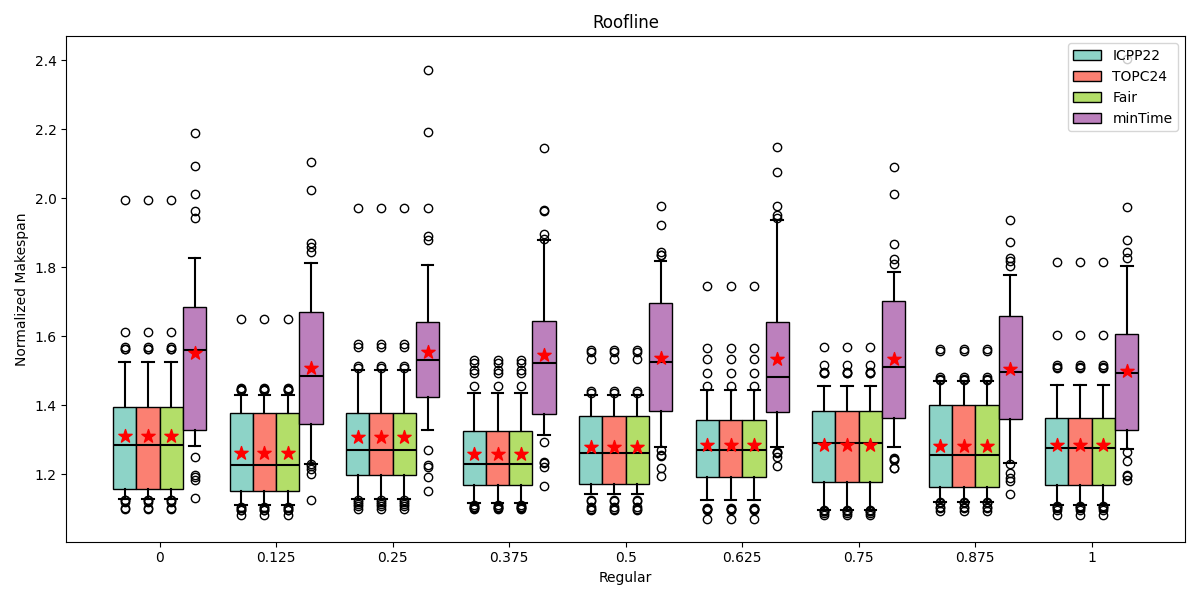
\includegraphics[width=\textwidth]{Results/Regular/Regular_Roofline_boxplot}\caption{Roofline}\label{fig:boxplot_figures_Regular_Roofline}\end{subfigure}
\hfill
\begin{subfigure}[b]{0.32\textwidth}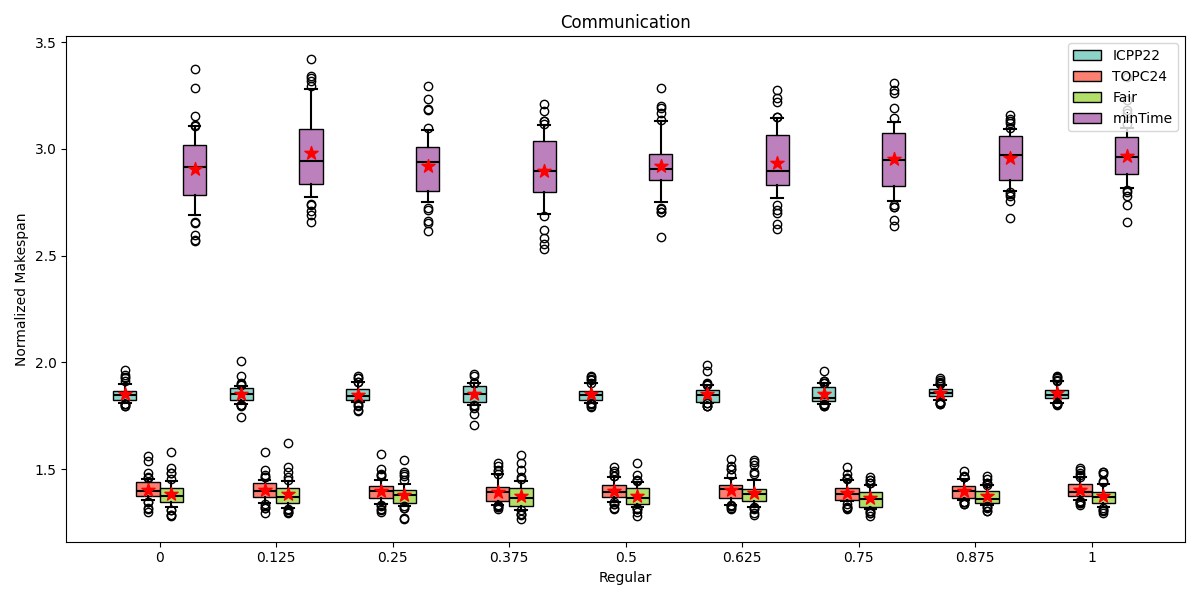
\includegraphics[width=\textwidth]{Results/Regular/Regular_Communication_boxplot}\caption{Communication}\label{fig:boxplot_figures_Regular_Communication}\end{subfigure}
\hfill
\begin{subfigure}[b]{0.32\textwidth}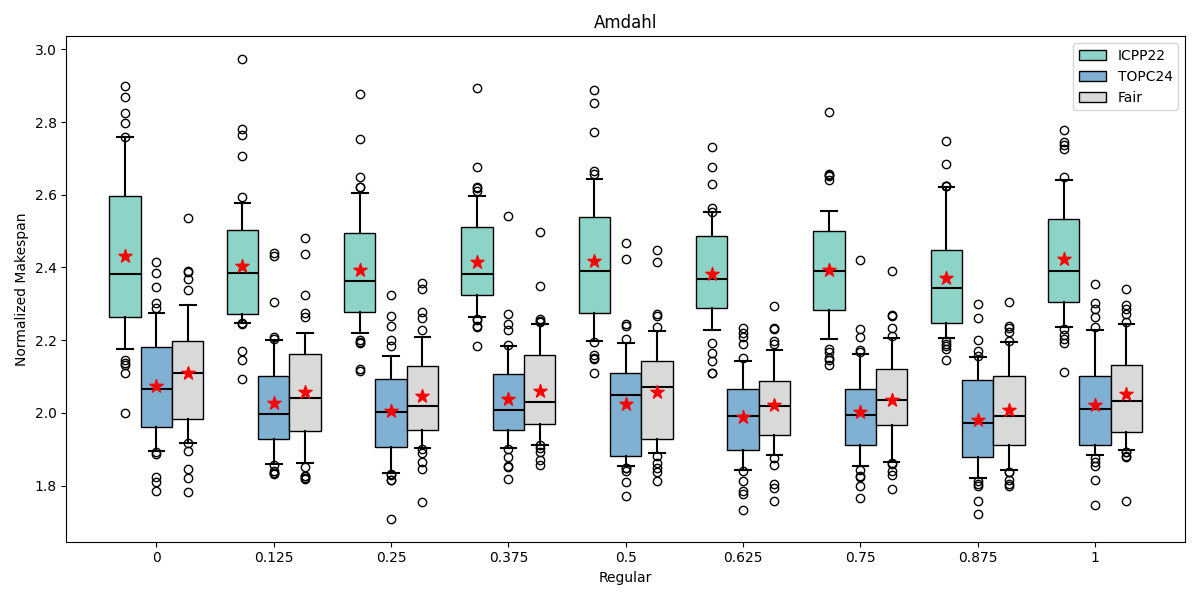
\includegraphics[width=\textwidth]{Results/Regular/Regular_Amdahl_boxplot}\caption{Amdahl}\label{fig:boxplot_figures_Regular_Amdahl}\end{subfigure}
\\[2ex]
\begin{subfigure}[b]{0.32\textwidth}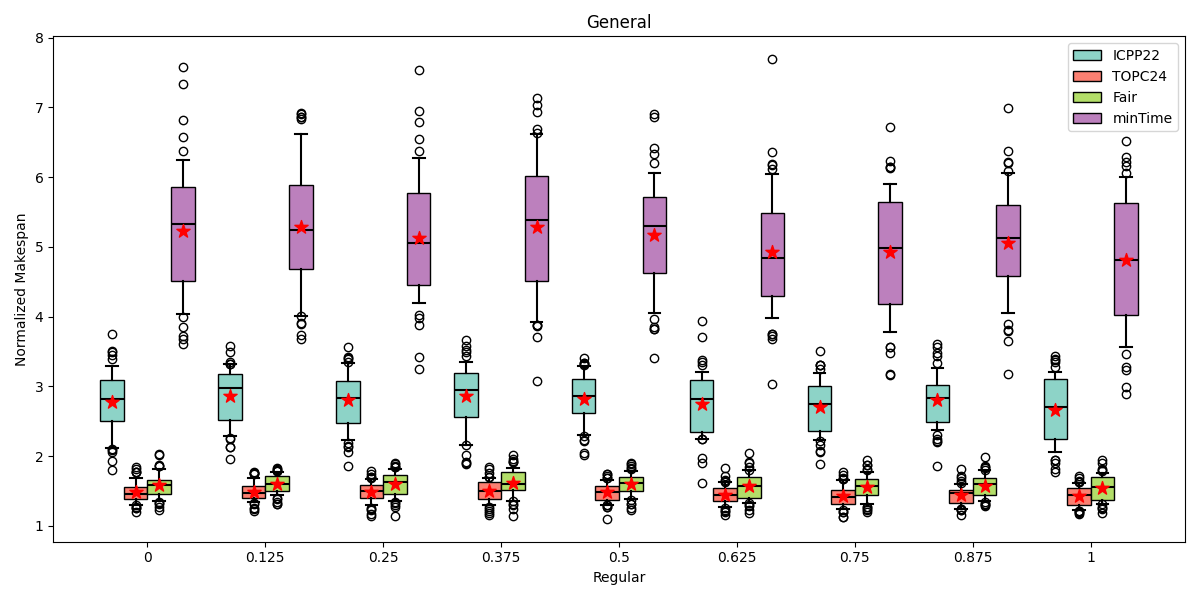
\includegraphics[width=\textwidth]{Results/Regular/Regular_General_boxplot}\caption{General}\label{fig:boxplot_figures_Regular_General}\end{subfigure}
\hfill
\begin{subfigure}[b]{0.32\textwidth}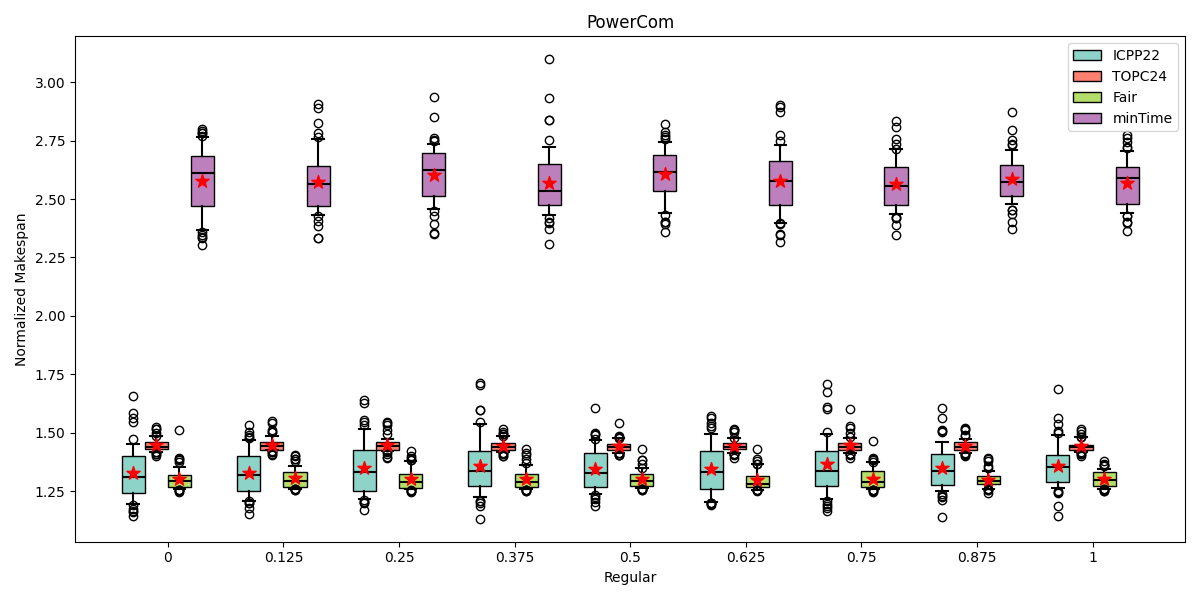
\includegraphics[width=\textwidth]{Results/Regular/Regular_PowerCom_boxplot}\caption{PowerCom}\label{fig:boxplot_figures_Regular_PowerCom}\end{subfigure}
\hfill
\caption{Boxplot Figure for Regular}
\label{fig:boxplot_figures_Regular}
\end{figure}
\begin{figure}[htbp]
\centering
\begin{subfigure}[b]{0.32\textwidth}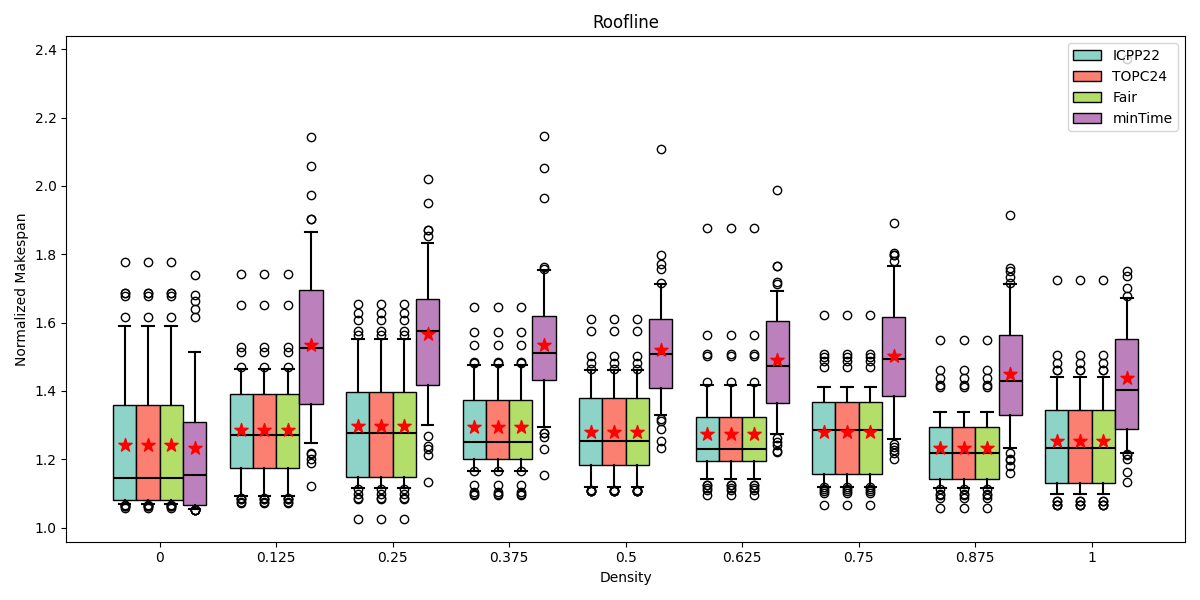
\includegraphics[width=\textwidth]{Results/Density/Density_Roofline_boxplot}\caption{Roofline}\label{fig:boxplot_figures_Density_Roofline}\end{subfigure}
\hfill
\begin{subfigure}[b]{0.32\textwidth}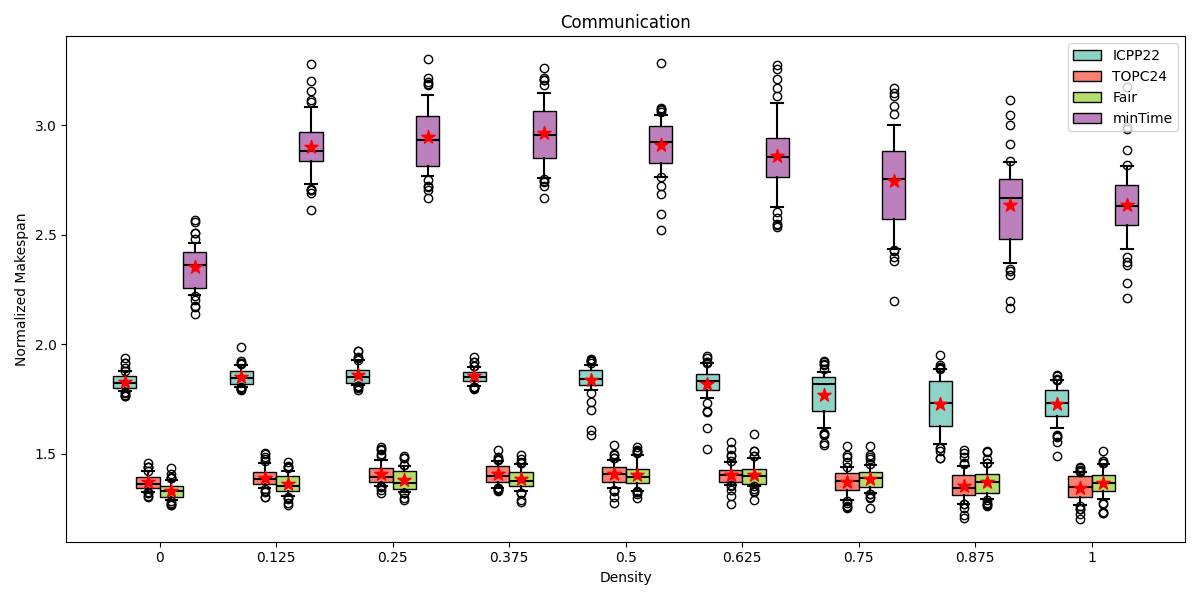
\includegraphics[width=\textwidth]{Results/Density/Density_Communication_boxplot}\caption{Communication}\label{fig:boxplot_figures_Density_Communication}\end{subfigure}
\hfill
\begin{subfigure}[b]{0.32\textwidth}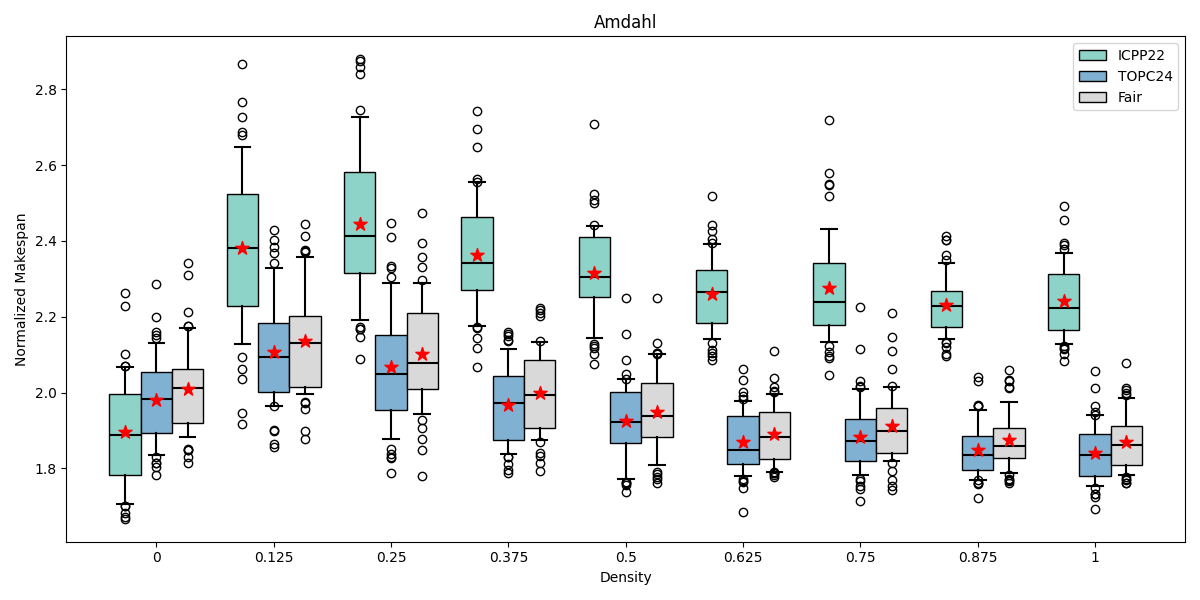
\includegraphics[width=\textwidth]{Results/Density/Density_Amdahl_boxplot}\caption{Amdahl}\label{fig:boxplot_figures_Density_Amdahl}\end{subfigure}
\\[2ex]
\begin{subfigure}[b]{0.32\textwidth}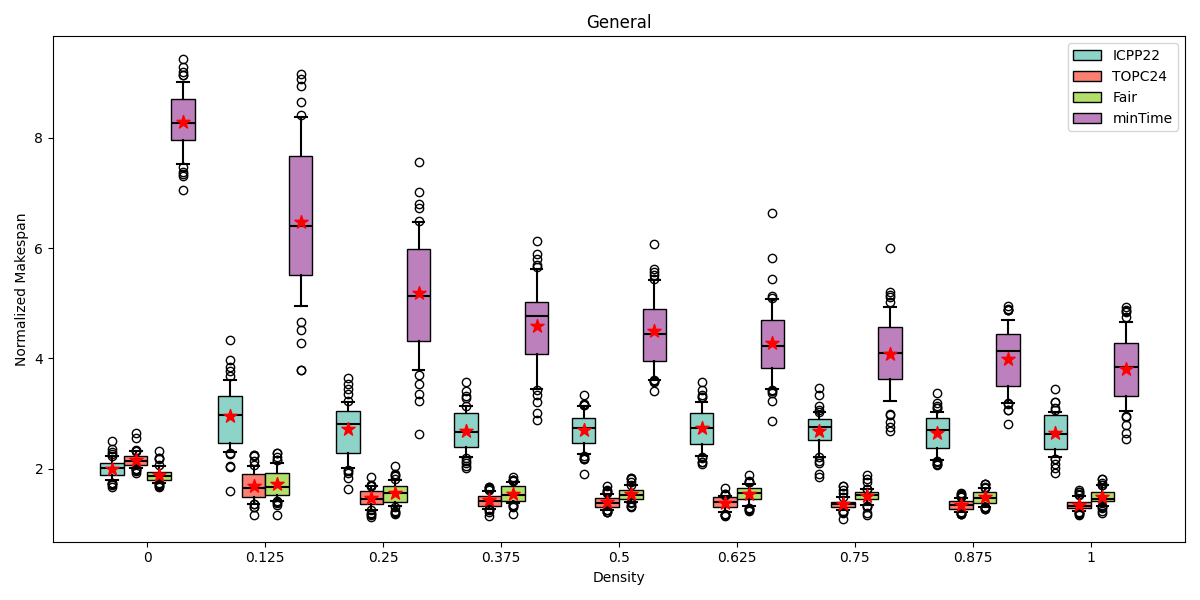
\includegraphics[width=\textwidth]{Results/Density/Density_General_boxplot}\caption{General}\label{fig:boxplot_figures_Density_General}\end{subfigure}
\hfill
\begin{subfigure}[b]{0.32\textwidth}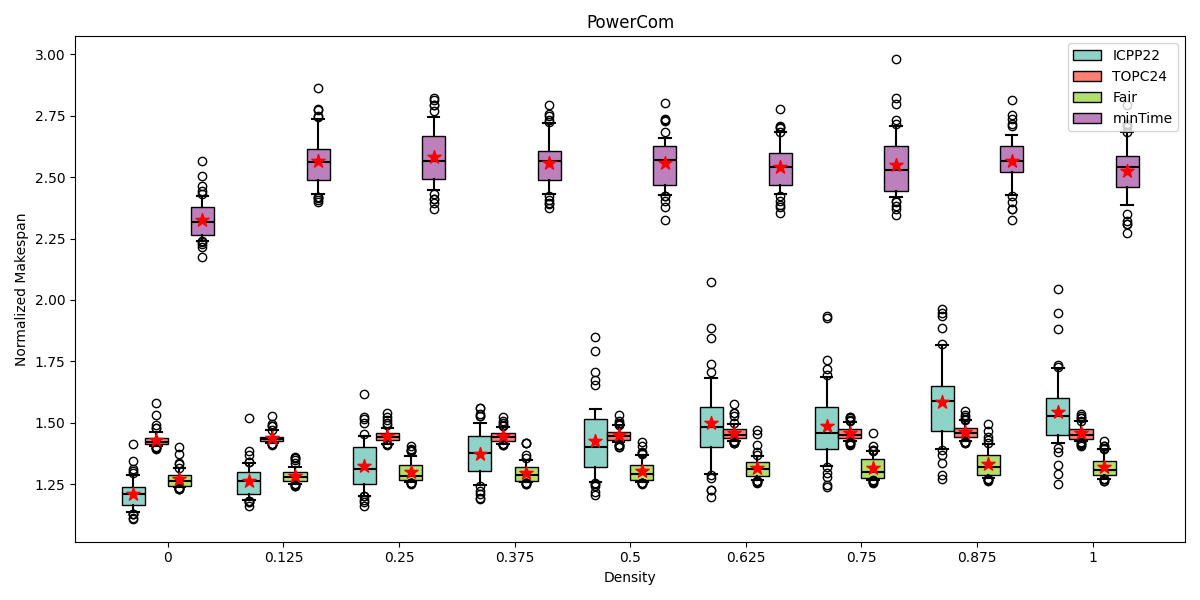
\includegraphics[width=\textwidth]{Results/Density/Density_PowerCom_boxplot}\caption{PowerCom}\label{fig:boxplot_figures_Density_PowerCom}\end{subfigure}
\hfill
\caption{Boxplot Figure for Density}
\label{fig:boxplot_figures_Density}
\end{figure}
\begin{figure}[htbp]
\centering
\begin{subfigure}[b]{0.32\textwidth}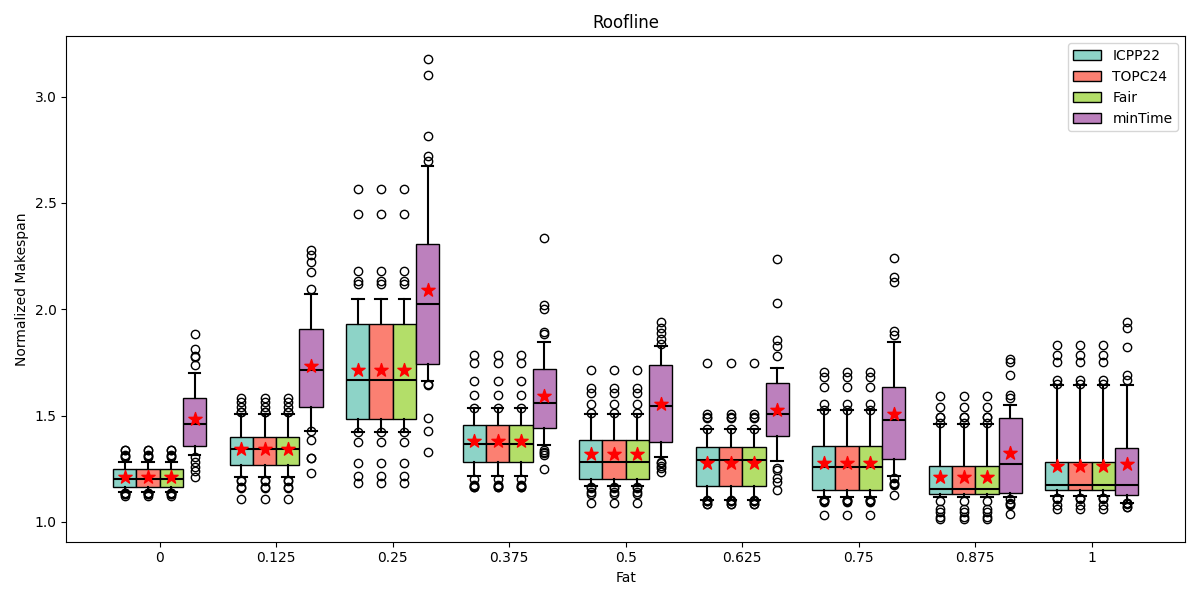
\includegraphics[width=\textwidth]{Results/Fat/Fat_Roofline_boxplot}\caption{Roofline}\label{fig:boxplot_figures_Fat_Roofline}\end{subfigure}
\hfill
\begin{subfigure}[b]{0.32\textwidth}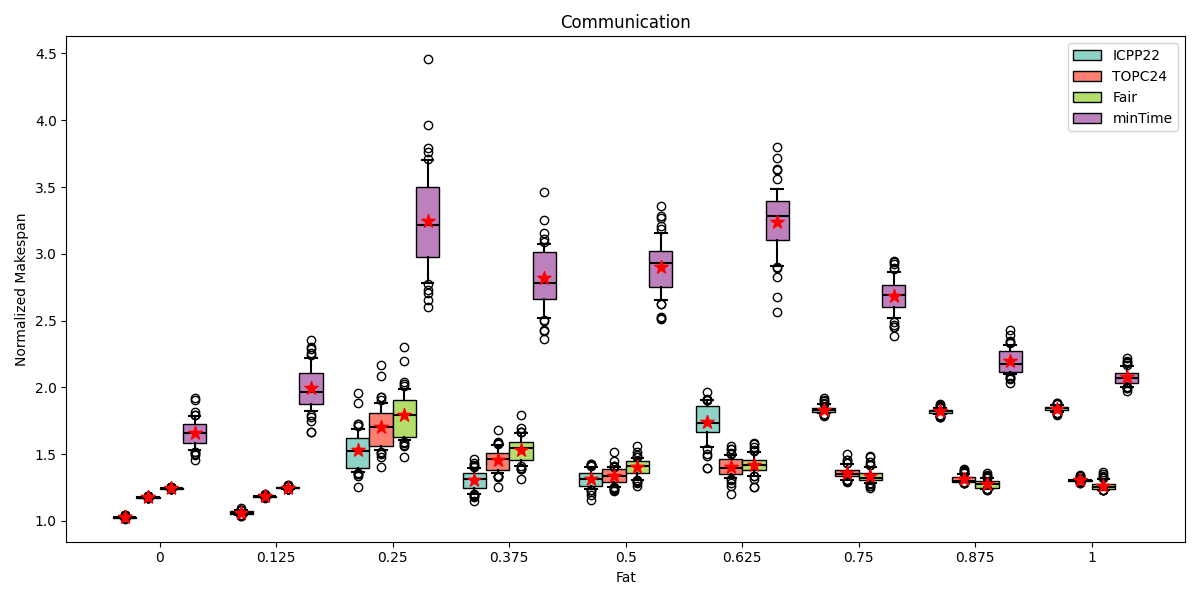
\includegraphics[width=\textwidth]{Results/Fat/Fat_Communication_boxplot}\caption{Communication}\label{fig:boxplot_figures_Fat_Communication}\end{subfigure}
\hfill
\begin{subfigure}[b]{0.32\textwidth}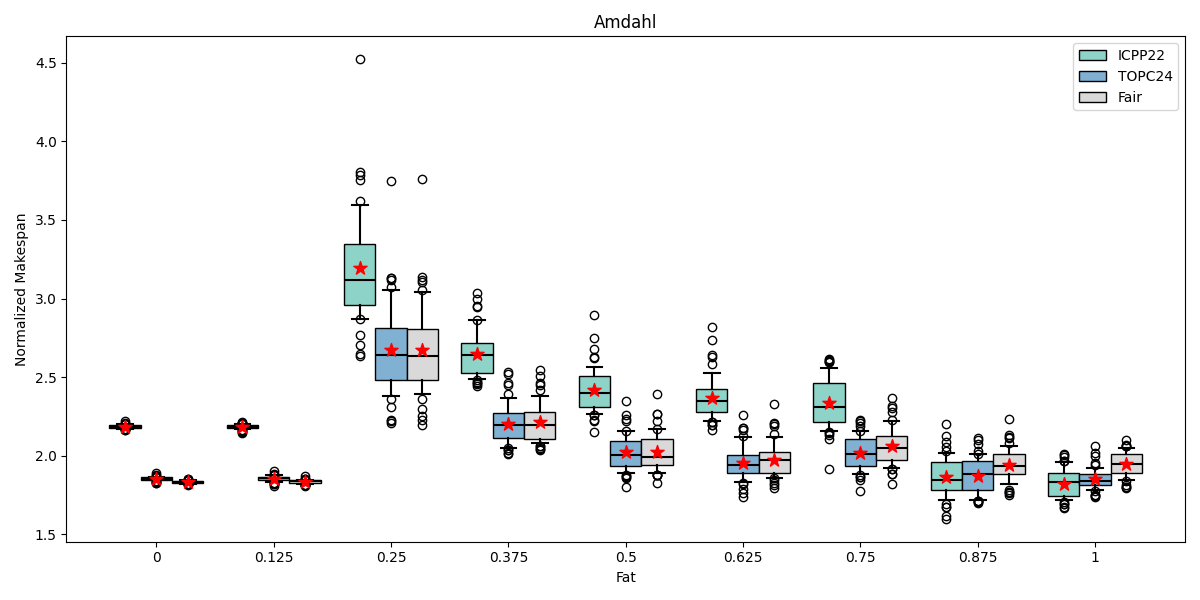
\includegraphics[width=\textwidth]{Results/Fat/Fat_Amdahl_boxplot}\caption{Amdahl}\label{fig:boxplot_figures_Fat_Amdahl}\end{subfigure}
\\[2ex]
\begin{subfigure}[b]{0.32\textwidth}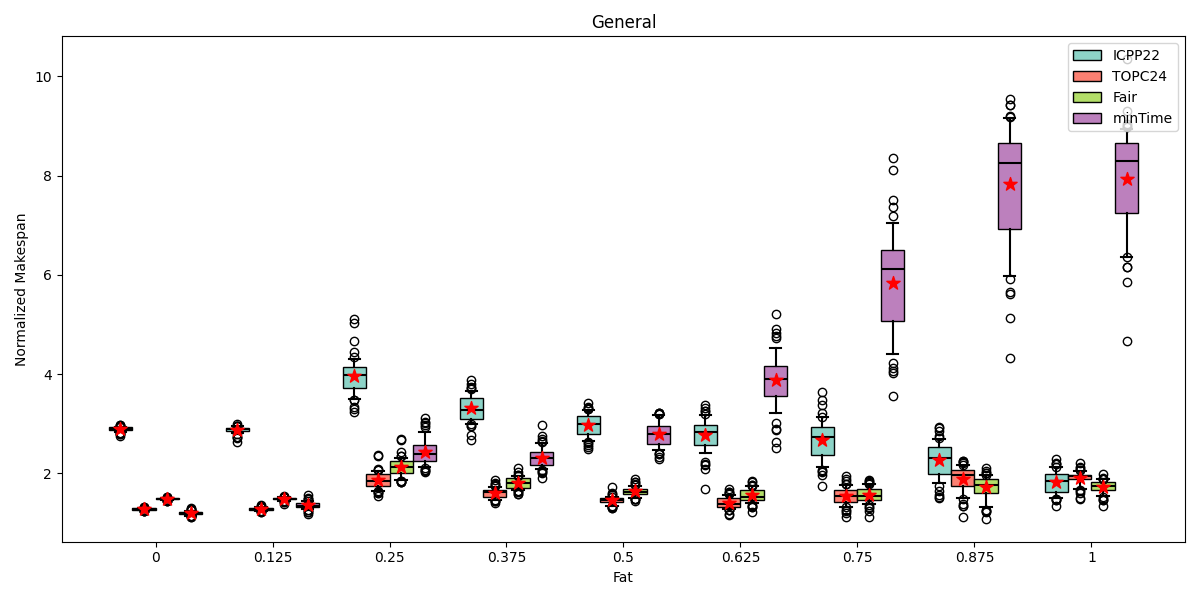
\includegraphics[width=\textwidth]{Results/Fat/Fat_General_boxplot}\caption{General}\label{fig:boxplot_figures_Fat_General}\end{subfigure}
\hfill
\begin{subfigure}[b]{0.32\textwidth}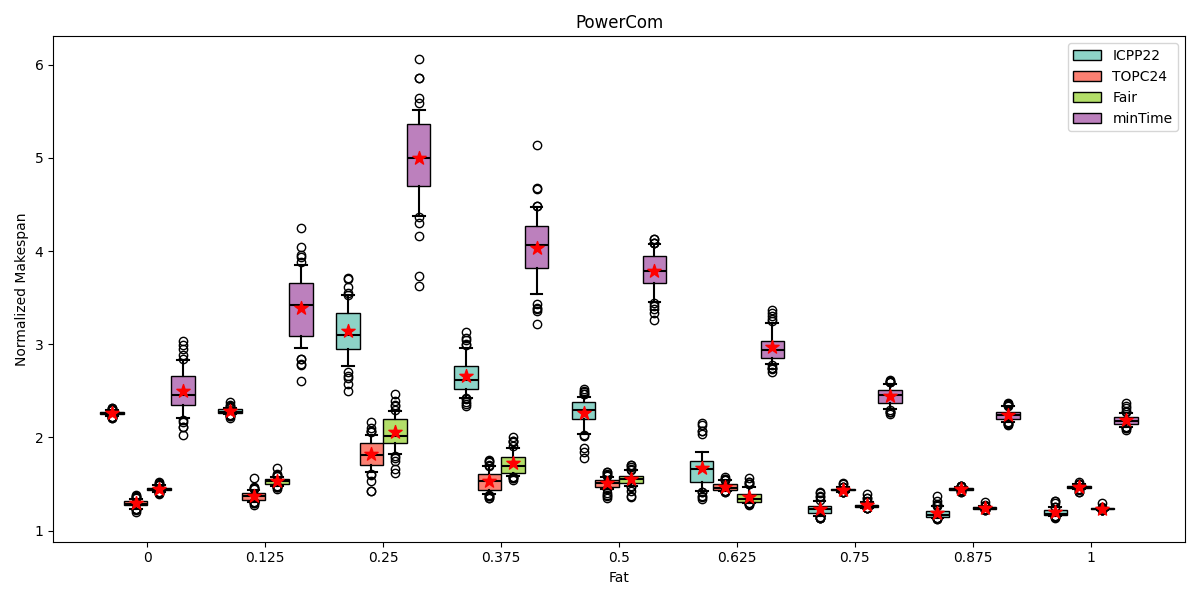
\includegraphics[width=\textwidth]{Results/Fat/Fat_PowerCom_boxplot}\caption{PowerCom}\label{fig:boxplot_figures_Fat_PowerCom}\end{subfigure}
\hfill
\caption{Boxplot Figure for Fat}
\label{fig:boxplot_figures_Fat}
\end{figure}
\begin{figure}[htbp]
\centering
\begin{subfigure}[b]{0.32\textwidth}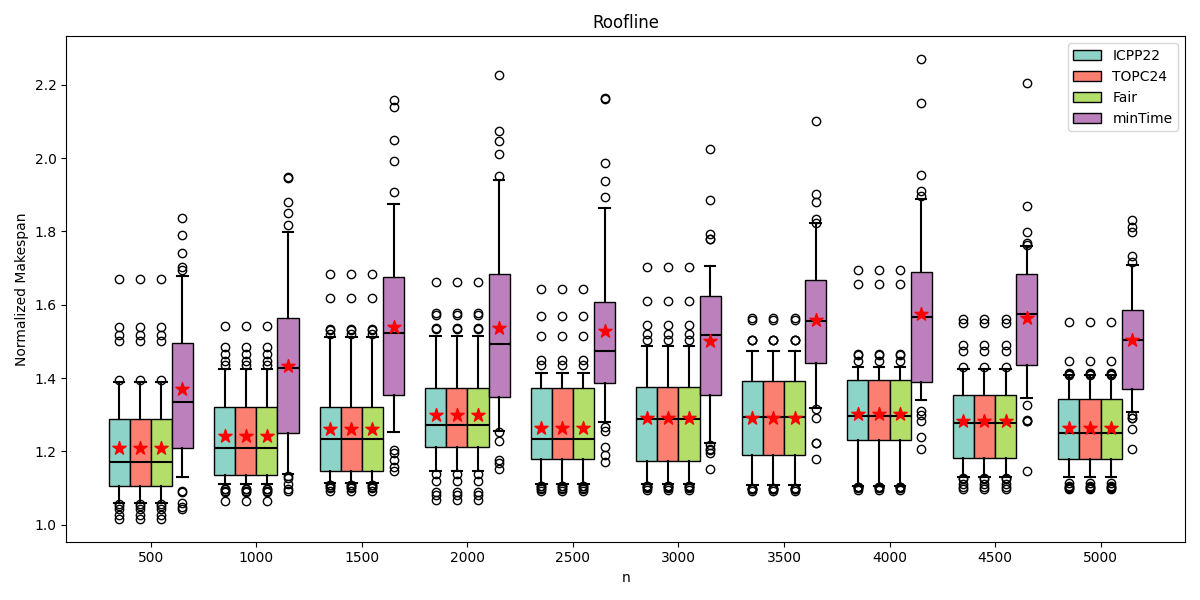
\includegraphics[width=\textwidth]{Results/n/n_Roofline_boxplot}\caption{Roofline}\label{fig:boxplot_figures_n_Roofline}\end{subfigure}
\hfill
\begin{subfigure}[b]{0.32\textwidth}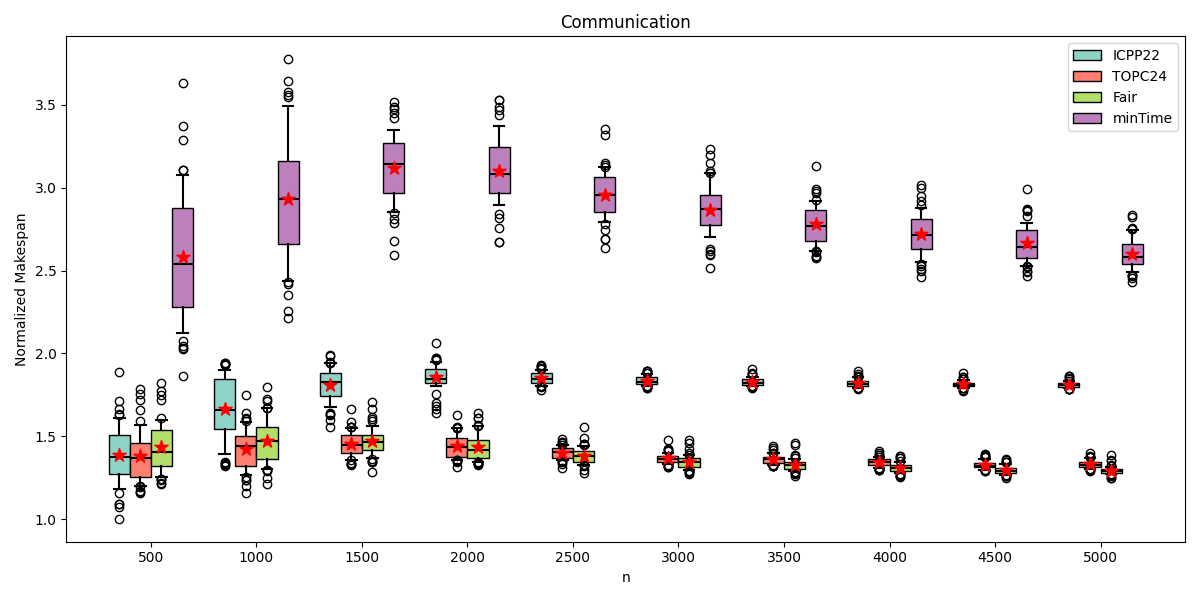
\includegraphics[width=\textwidth]{Results/n/n_Communication_boxplot}\caption{Communication}\label{fig:boxplot_figures_n_Communication}\end{subfigure}
\hfill
\begin{subfigure}[b]{0.32\textwidth}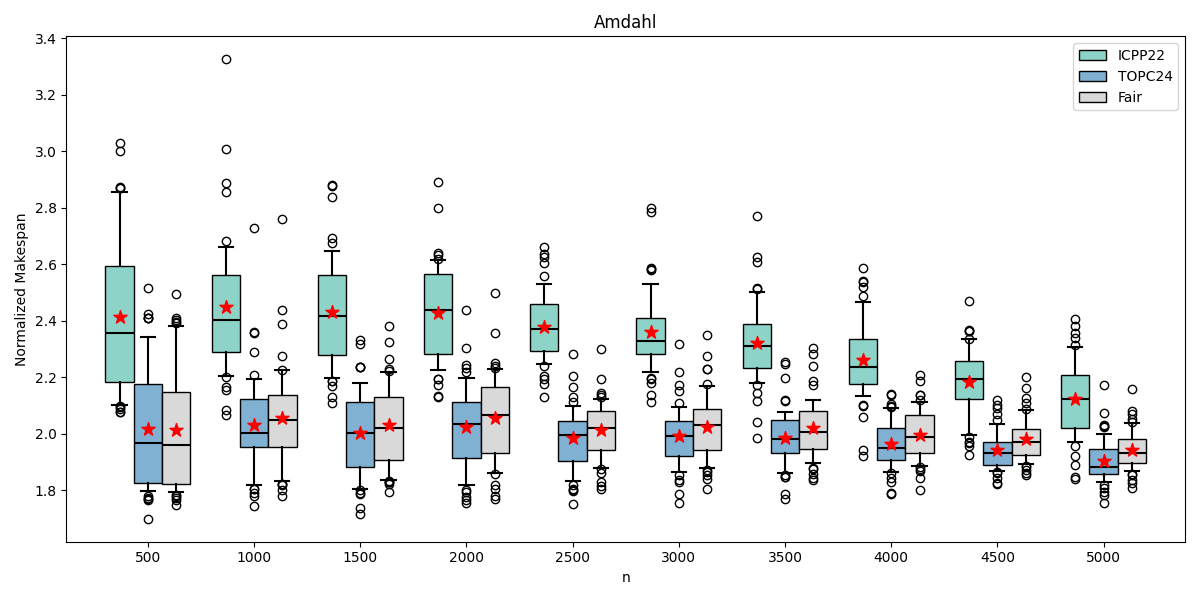
\includegraphics[width=\textwidth]{Results/n/n_Amdahl_boxplot}\caption{Amdahl}\label{fig:boxplot_figures_n_Amdahl}\end{subfigure}
\\[2ex]
\begin{subfigure}[b]{0.32\textwidth}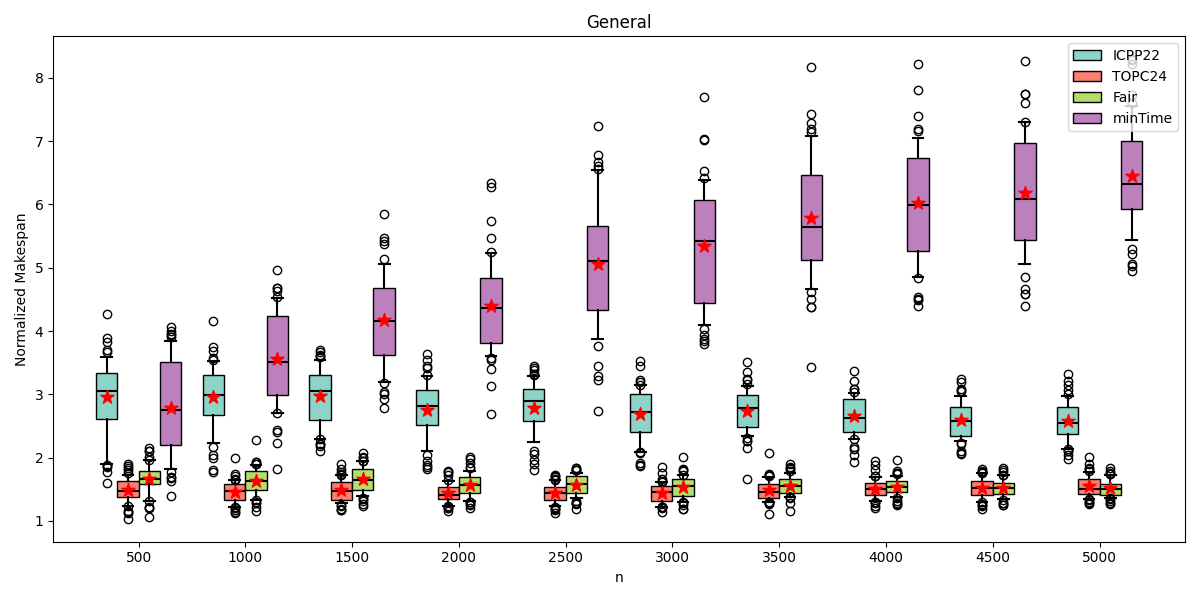
\includegraphics[width=\textwidth]{Results/n/n_General_boxplot}\caption{General}\label{fig:boxplot_figures_n_General}\end{subfigure}
\hfill
\begin{subfigure}[b]{0.32\textwidth}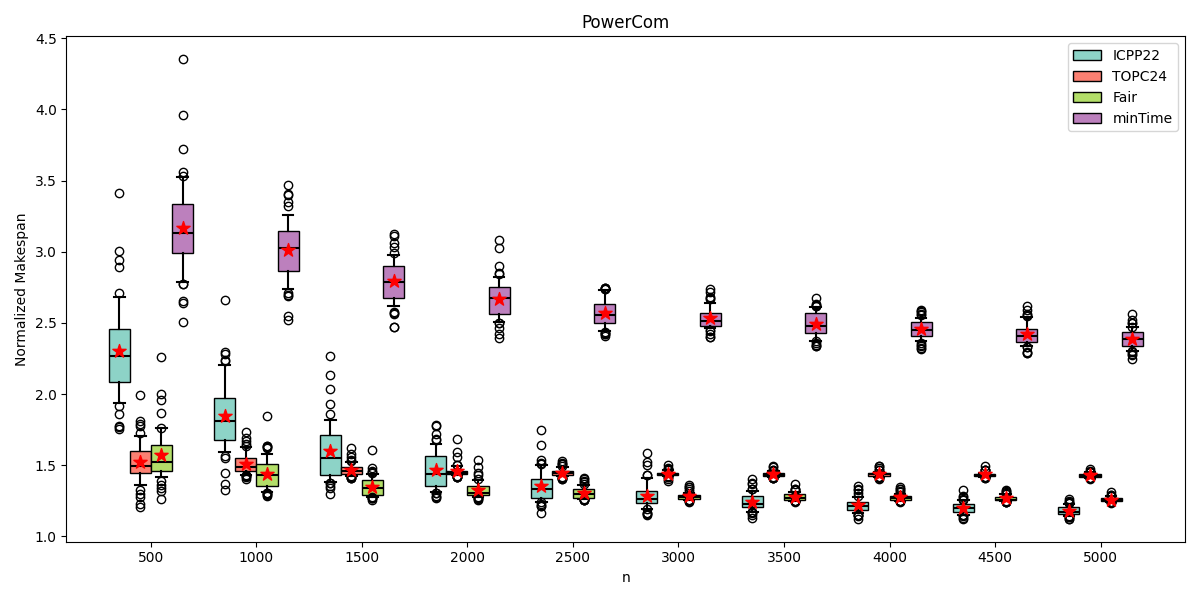
\includegraphics[width=\textwidth]{Results/n/n_PowerCom_boxplot}\caption{PowerCom}\label{fig:boxplot_figures_n_PowerCom}\end{subfigure}
\hfill
\caption{Boxplot Figure for n}
\label{fig:boxplot_figures_n}
\end{figure}
\begin{figure}[htbp]
\centering
\begin{subfigure}[b]{0.32\textwidth}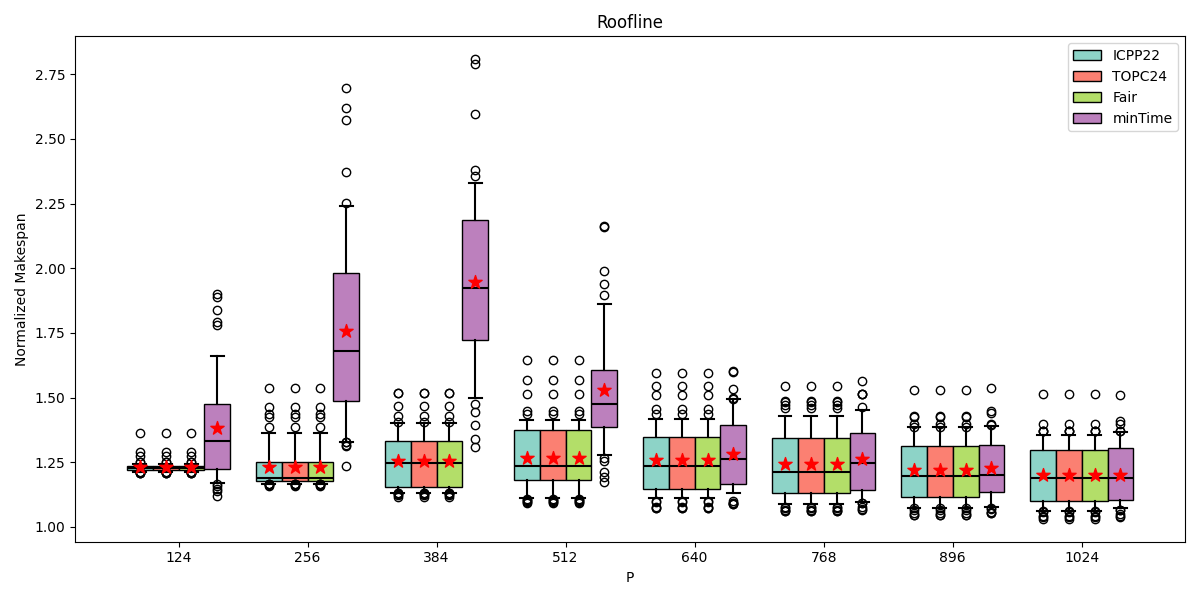
\includegraphics[width=\textwidth]{Results/P/P_Roofline_boxplot}\caption{Roofline}\label{fig:boxplot_figures_P_Roofline}\end{subfigure}
\hfill
\begin{subfigure}[b]{0.32\textwidth}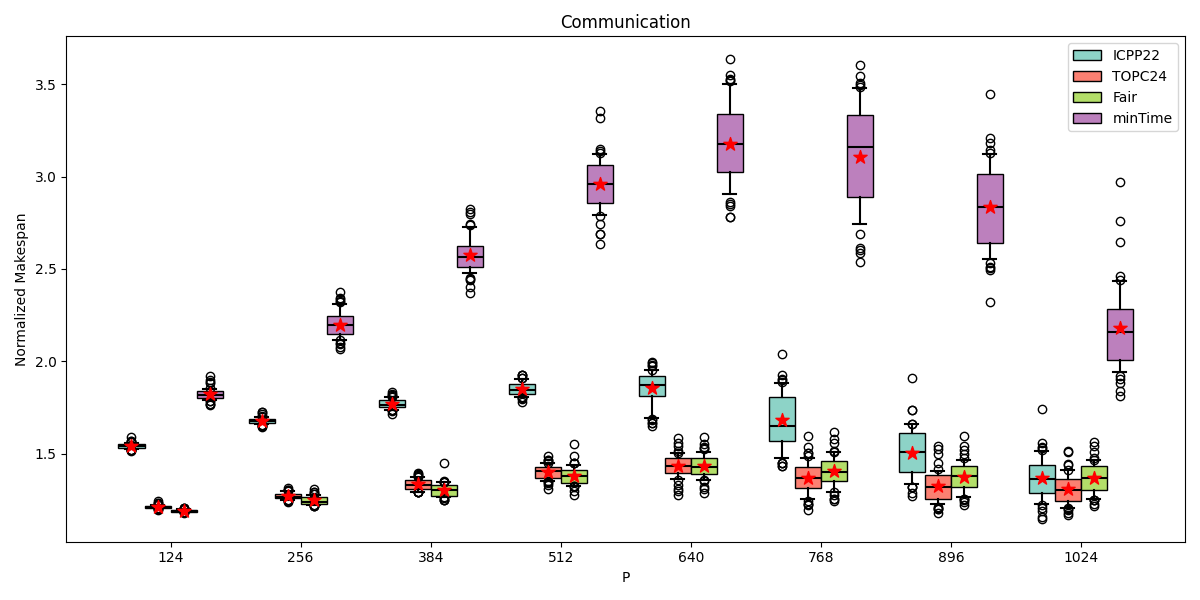
\includegraphics[width=\textwidth]{Results/P/P_Communication_boxplot}\caption{Communication}\label{fig:boxplot_figures_P_Communication}\end{subfigure}
\hfill
\begin{subfigure}[b]{0.32\textwidth}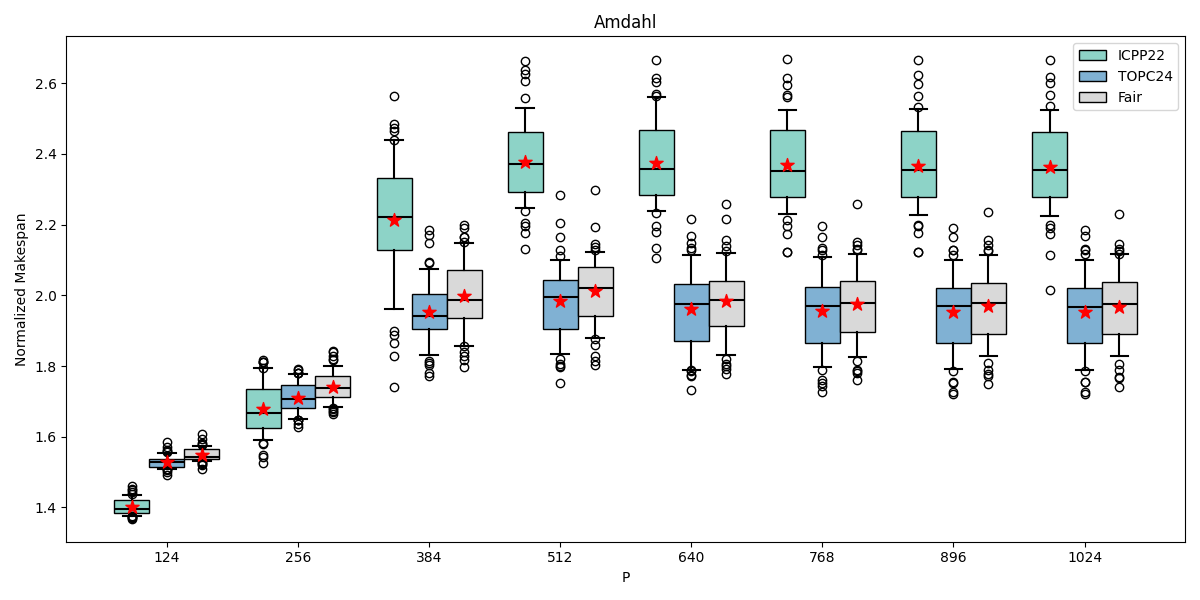
\includegraphics[width=\textwidth]{Results/P/P_Amdahl_boxplot}\caption{Amdahl}\label{fig:boxplot_figures_P_Amdahl}\end{subfigure}
\\[2ex]
\begin{subfigure}[b]{0.32\textwidth}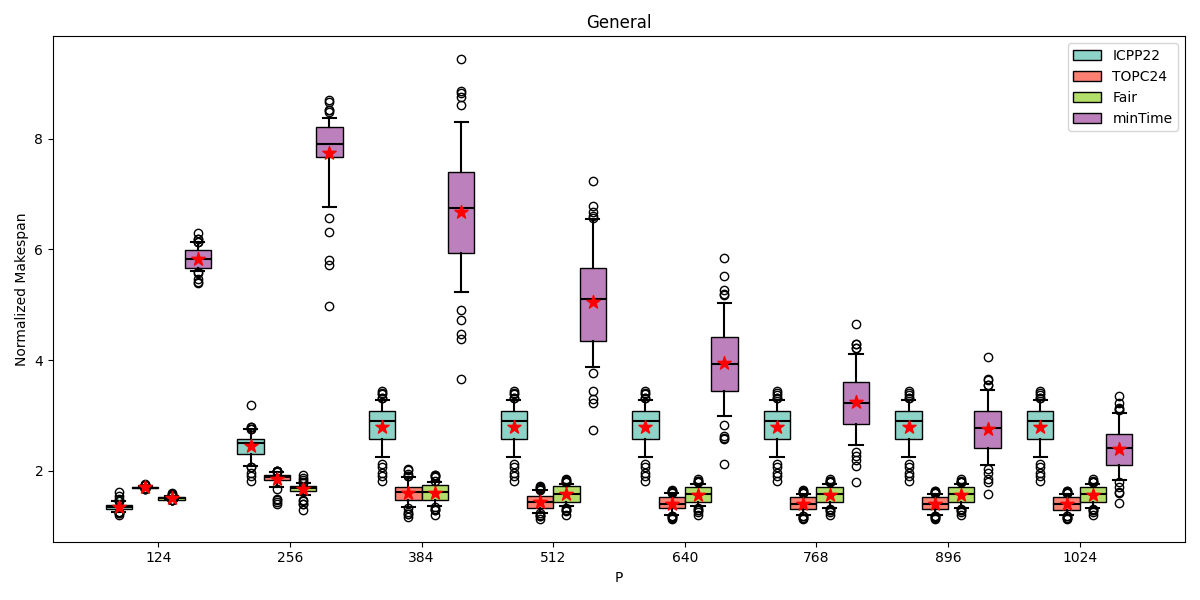
\includegraphics[width=\textwidth]{Results/P/P_General_boxplot}\caption{General}\label{fig:boxplot_figures_P_General}\end{subfigure}
\hfill
\begin{subfigure}[b]{0.32\textwidth}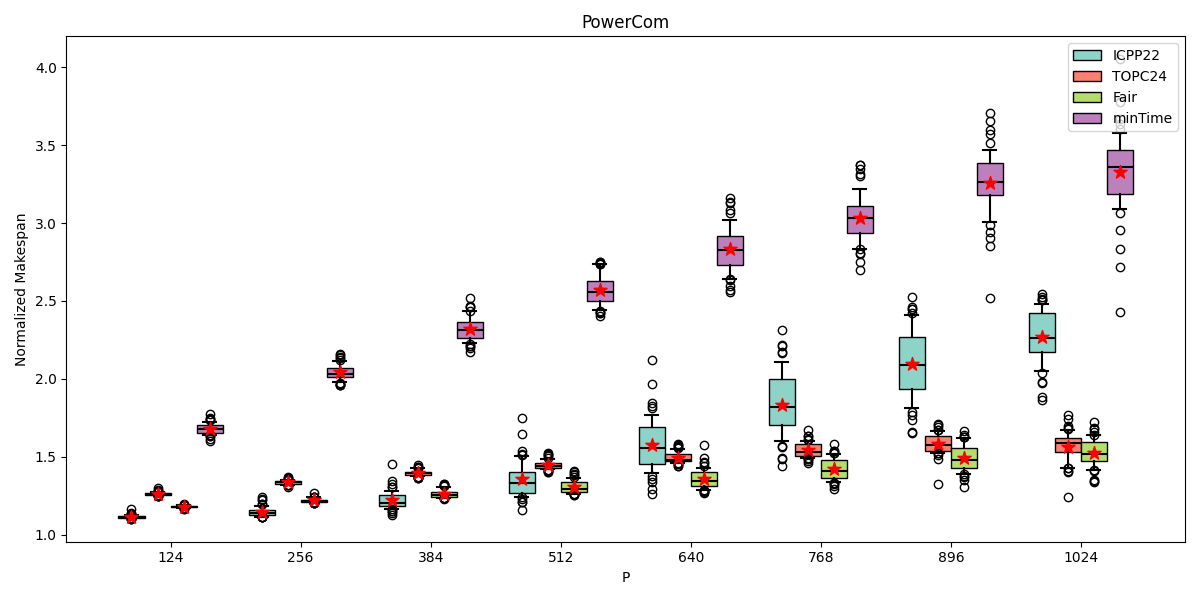
\includegraphics[width=\textwidth]{Results/P/P_PowerCom_boxplot}\caption{PowerCom}\label{fig:boxplot_figures_P_PowerCom}\end{subfigure}
\hfill
\caption{Boxplot Figure for P}
\label{fig:boxplot_figures_P}
\end{figure}
\begin{figure}[htbp]
\centering
\begin{subfigure}[b]{0.32\textwidth}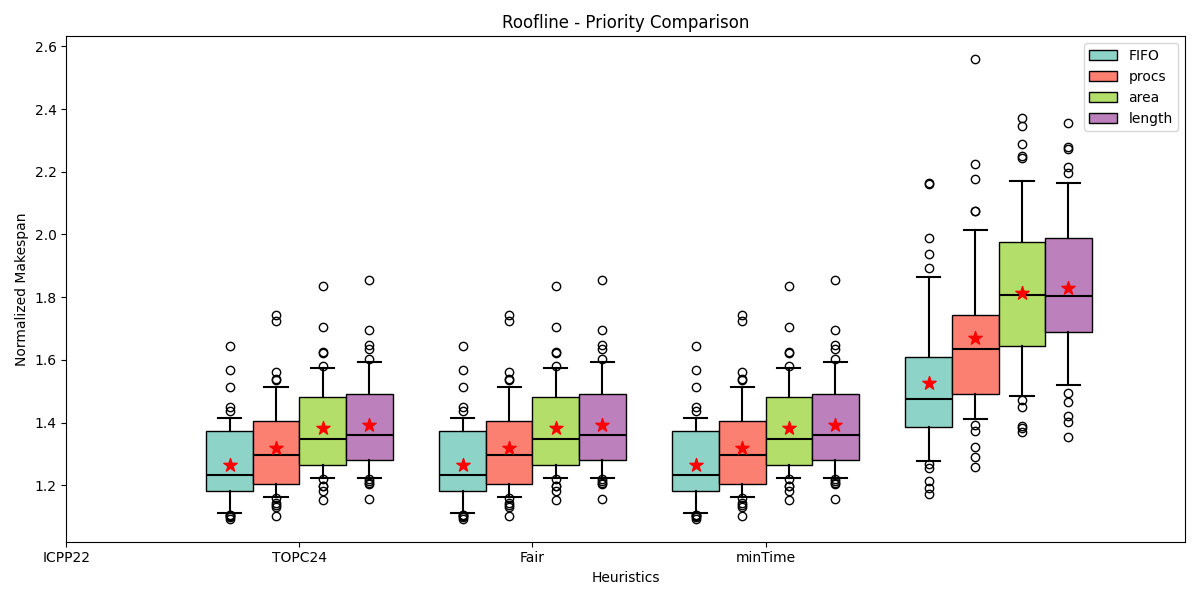
\includegraphics[width=\textwidth]{Results/Priority/Priority_Roofline_boxplot}\caption{Roofline}\label{fig:boxplot_figures_Priority_Roofline}\end{subfigure}
\hfill
\begin{subfigure}[b]{0.32\textwidth}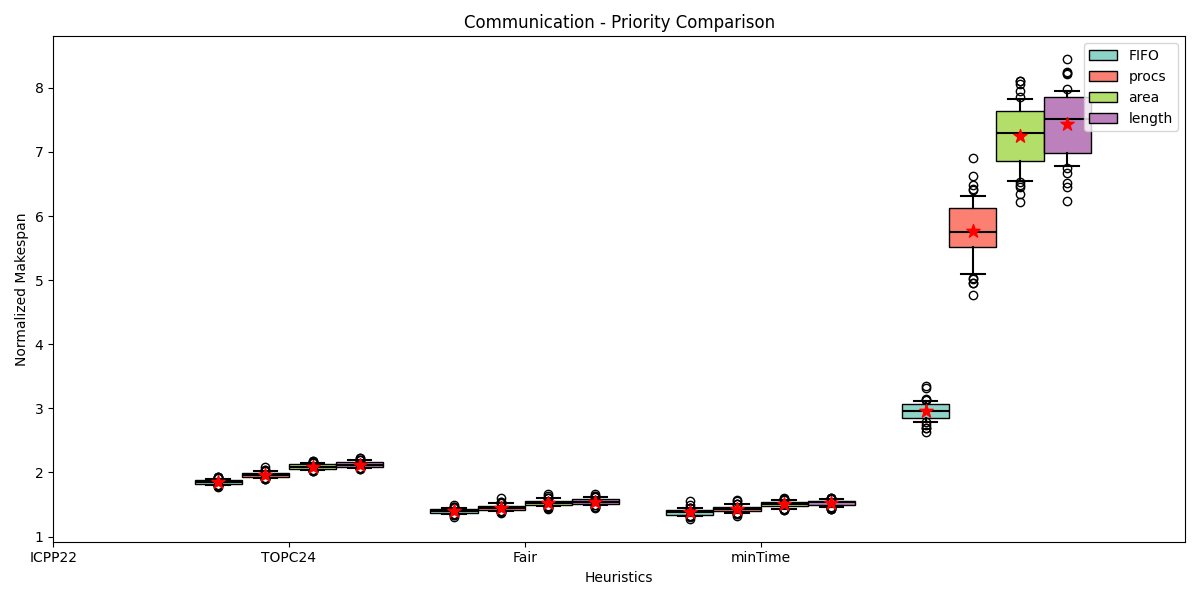
\includegraphics[width=\textwidth]{Results/Priority/Priority_Communication_boxplot}\caption{Communication}\label{fig:boxplot_figures_Priority_Communication}\end{subfigure}
\hfill
\begin{subfigure}[b]{0.32\textwidth}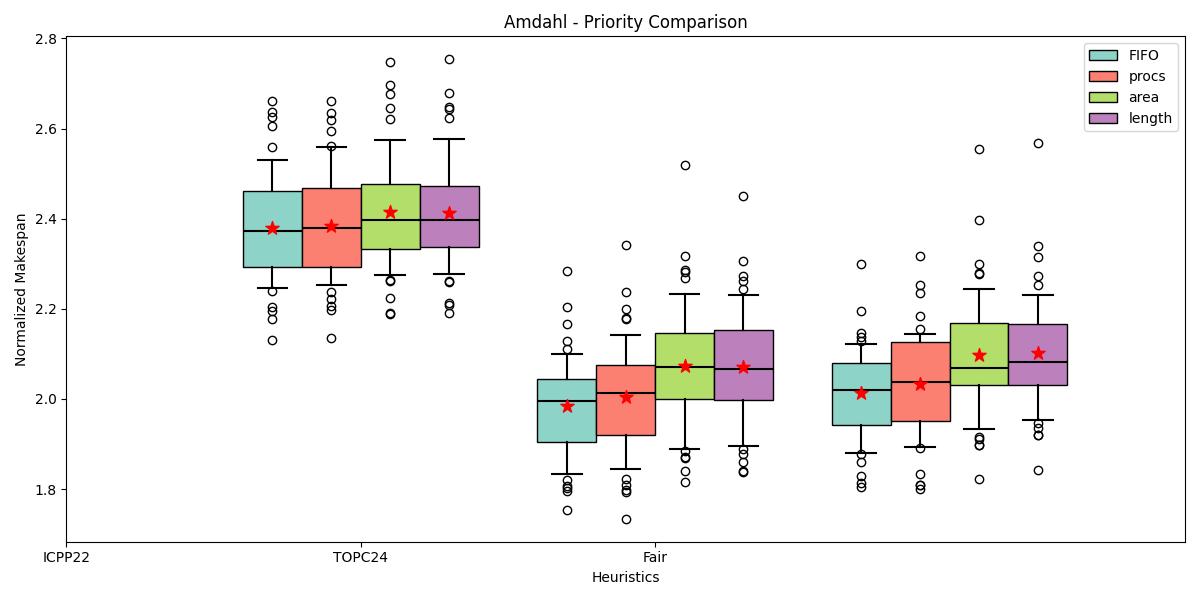
\includegraphics[width=\textwidth]{Results/Priority/Priority_Amdahl_boxplot}\caption{Amdahl}\label{fig:boxplot_figures_Priority_Amdahl}\end{subfigure}
\\[2ex]
\begin{subfigure}[b]{0.32\textwidth}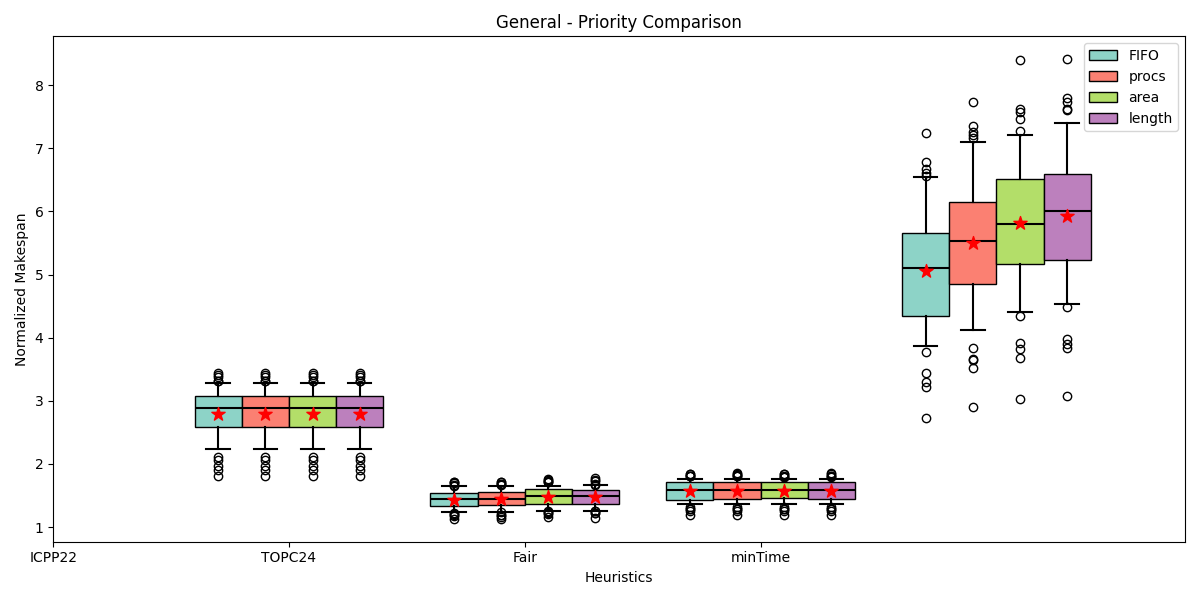
\includegraphics[width=\textwidth]{Results/Priority/Priority_General_boxplot}\caption{General}\label{fig:boxplot_figures_Priority_General}\end{subfigure}
\hfill
\begin{subfigure}[b]{0.32\textwidth}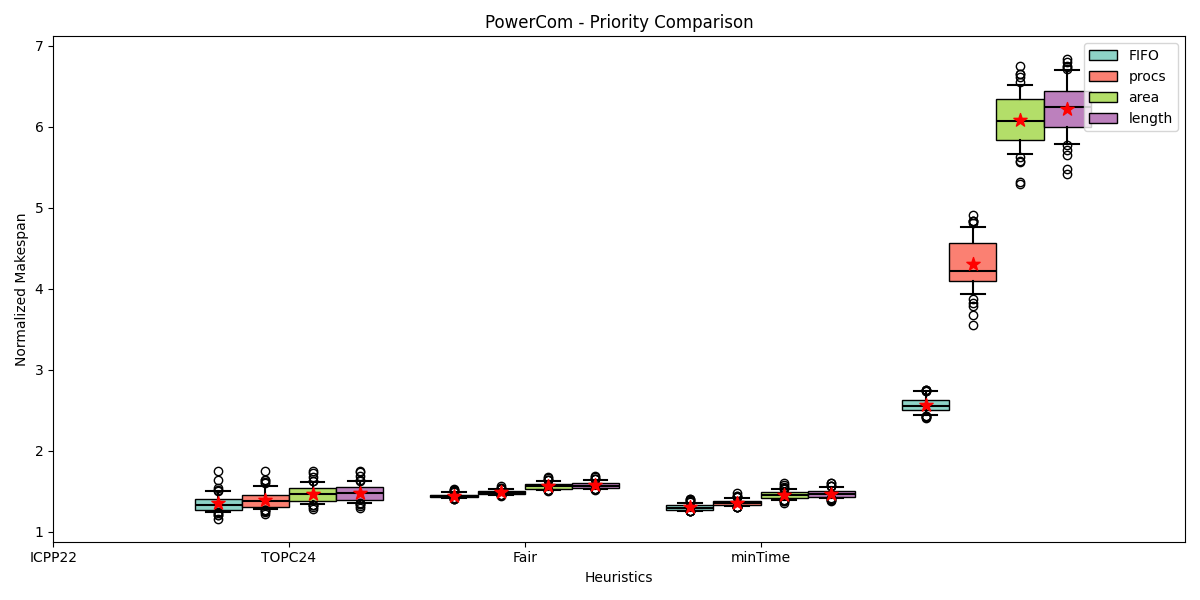
\includegraphics[width=\textwidth]{Results/Priority/Priority_PowerCom_boxplot}\caption{PowerCom}\label{fig:boxplot_figures_Priority_PowerCom}\end{subfigure}
\hfill
\caption{Boxplot Figure for Priority}
\label{fig:boxplot_figures_Priority}
\end{figure}
\begin{figure}[htbp]
\centering
\begin{subfigure}[b]{0.32\textwidth}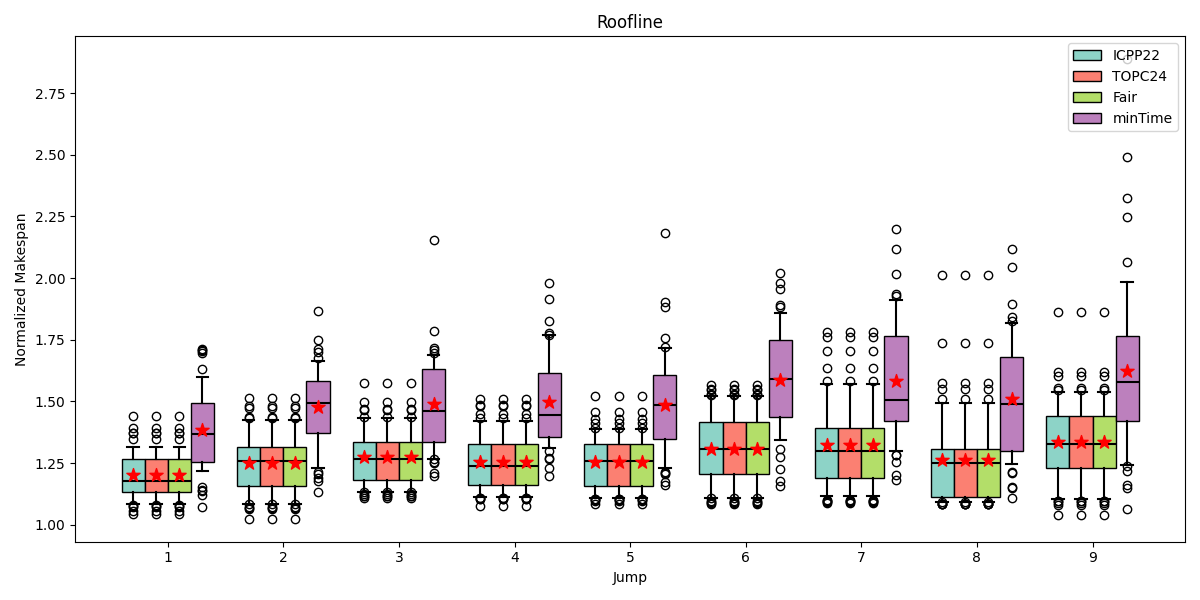
\includegraphics[width=\textwidth]{Results/Jump/Jump_Roofline_boxplot}\caption{Roofline}\label{fig:boxplot_figures_Jump_Roofline}\end{subfigure}
\hfill
\begin{subfigure}[b]{0.32\textwidth}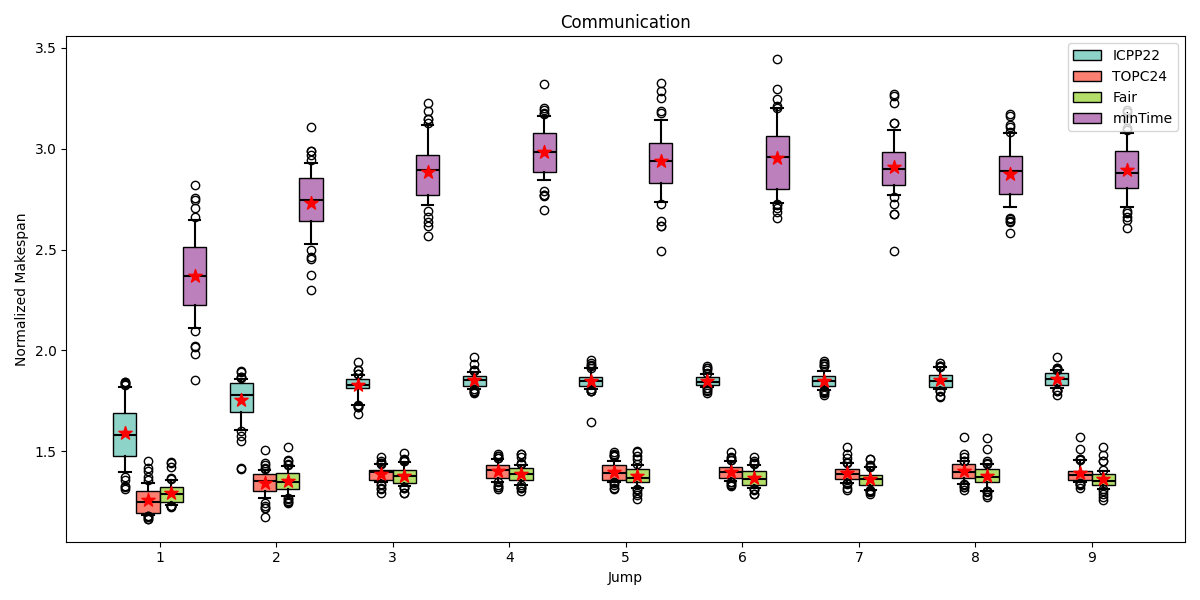
\includegraphics[width=\textwidth]{Results/Jump/Jump_Communication_boxplot}\caption{Communication}\label{fig:boxplot_figures_Jump_Communication}\end{subfigure}
\hfill
\begin{subfigure}[b]{0.32\textwidth}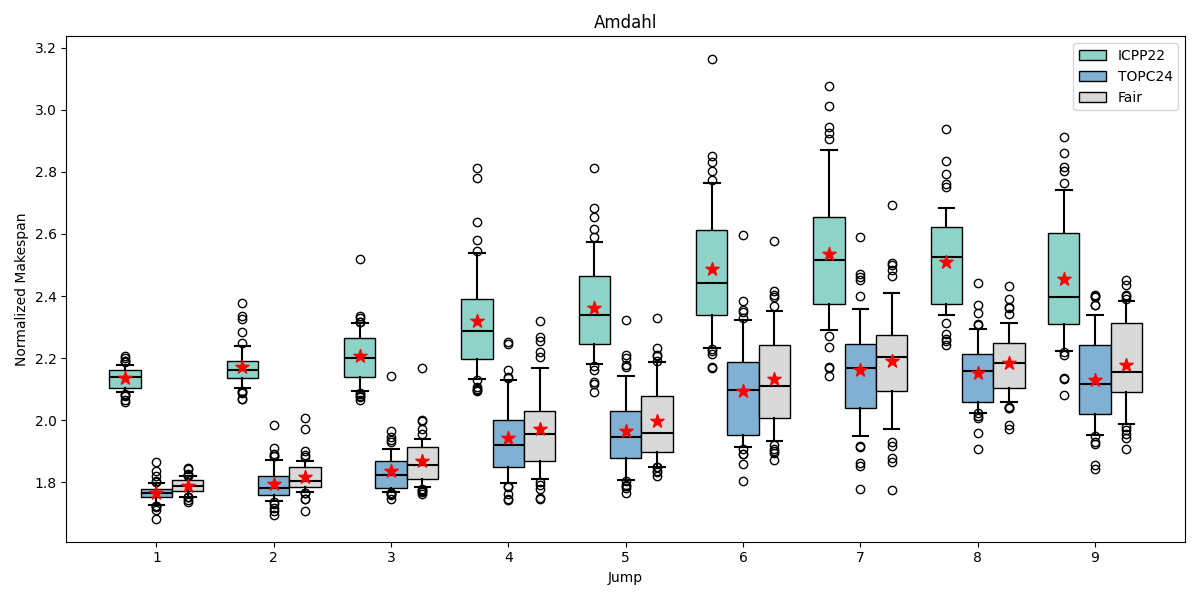
\includegraphics[width=\textwidth]{Results/Jump/Jump_Amdahl_boxplot}\caption{Amdahl}\label{fig:boxplot_figures_Jump_Amdahl}\end{subfigure}
\\[2ex]
\begin{subfigure}[b]{0.32\textwidth}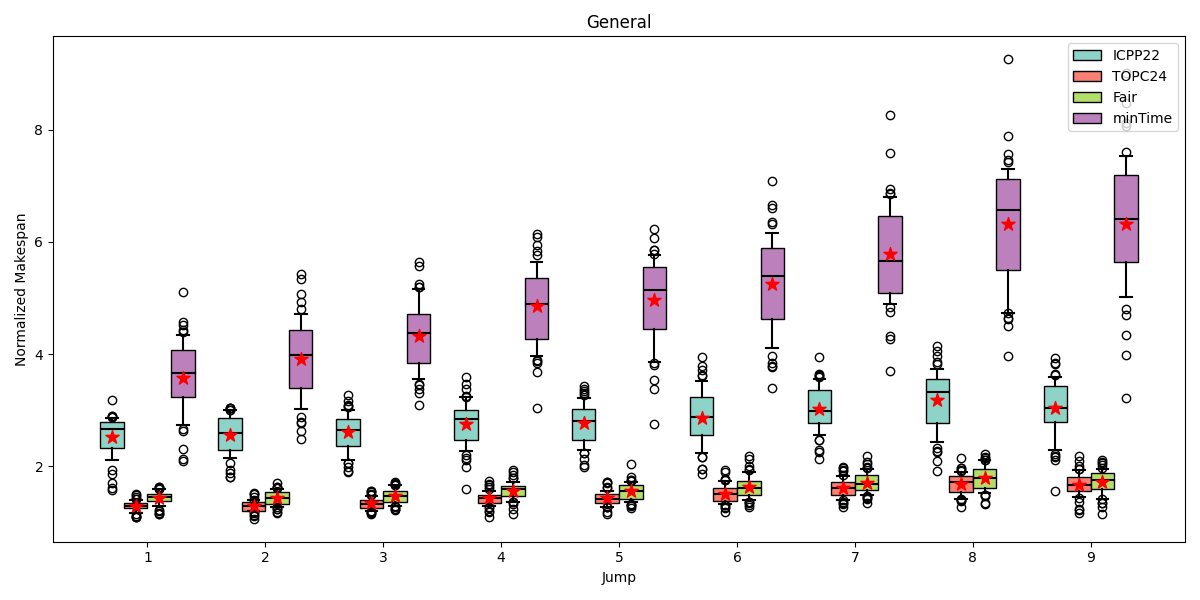
\includegraphics[width=\textwidth]{Results/Jump/Jump_General_boxplot}\caption{General}\label{fig:boxplot_figures_Jump_General}\end{subfigure}
\hfill
\begin{subfigure}[b]{0.32\textwidth}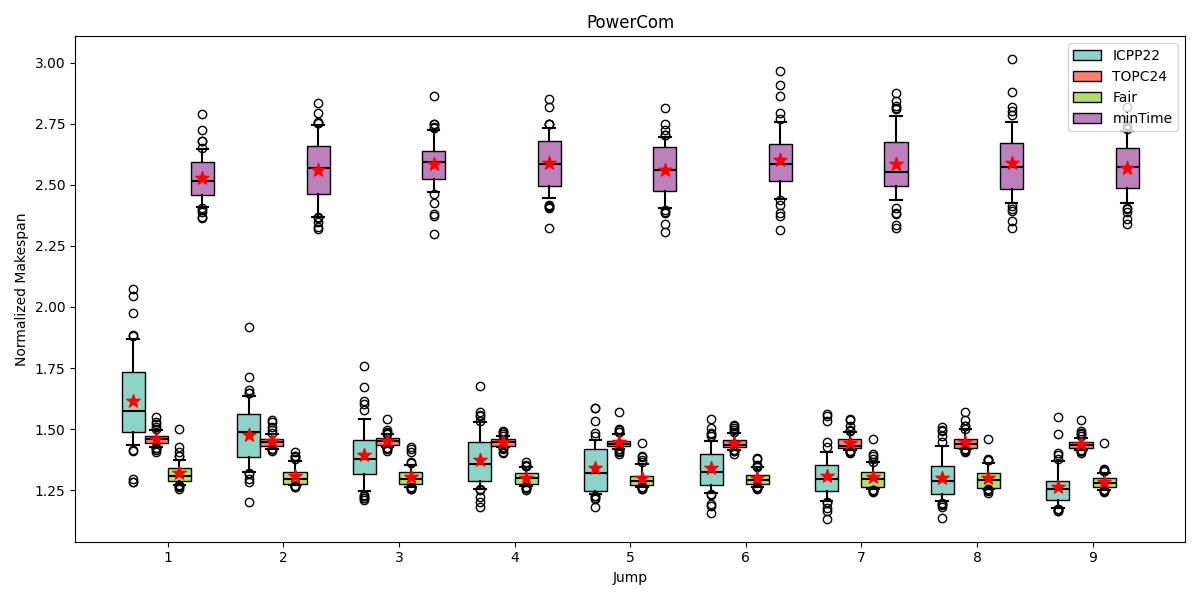
\includegraphics[width=\textwidth]{Results/Jump/Jump_PowerCom_boxplot}\caption{PowerCom}\label{fig:boxplot_figures_Jump_PowerCom}\end{subfigure}
\hfill
\caption{Boxplot Figure for Jump}
\label{fig:boxplot_figures_Jump}
\end{figure}


\FloatBarrier 

\subsection{Average Values}
\begin{table}[htbp]
\centering
\caption{Average Values for Each Model and Heuristic}
\label{tab:average_values}
\begin{tabular}{lrrrrr}
\toprule
Model & ICPP22 & TOPC24 & Fair & minTime & minArea \\
Roofline & 1.28 & 1.28 & 1.28 & 1.52 & 11.28 \\
Communication & 1.75 & 1.38 & 1.38 & 2.97 & 10.22 \\
Amdahl & 2.32 & 1.98 & 2.01 & 21.31 & 7.88 \\
General & 2.74 & 1.50 & 1.60 & 4.86 & 5.37 \\
PowerCom & 1.52 & 1.46 & 1.35 & 2.84 & 12.76 \\
\midrule
Average & 1.92 & 1.52 & 1.52 & 6.70 & 9.50 \\
\bottomrule
\end{tabular}
\end{table}

\subsection{Maximum Values}
\begin{table}[htbp]
\centering
\caption{Maximum Values for Each Model and Heuristic}
\label{tab:maximum_values}
\begin{tabular}{lrrrrr}
\toprule
Model & ICPP22 & TOPC24 & Fair & minTime & minArea \\
Roofline & 2.56 & 2.56 & 2.56 & 3.18 & 117.75 \\
Communication & 2.22 & 2.17 & 2.30 & 8.45 & 34.30 \\
Amdahl & 4.52 & 3.75 & 3.76 & 33.26 & 23.45 \\
General & 5.11 & 2.64 & 2.70 & 10.34 & 14.76 \\
PowerCom & 3.71 & 2.16 & 2.46 & 6.83 & 69.98 \\
\midrule
Maximum & 5.11 & 3.75 & 3.76 & 33.26 & 117.75 \\
\bottomrule
\end{tabular}
\end{table}


\FloatBarrier 

\bibliographystyle{plain}
\bibliography{moldable}

\end{document}
